
\import{}{EoS.tex}
\newpage

\section{Parameters}


\begin{table}[]
\caption{Pure component parameters in the CPA and eCPA EoS \cite{Tsivintzelis2011,Maribo2015}.$^a$ }
\centering
\adjustbox{max width=\textwidth}{
\begin{tabular}{ccccccccccccc}
\hline
\hline
 \textbf{Component} & $a_{0i}$ & $c_{1i}$ & $b_i$ & $\epsilon_{i}/k_B$ & $\kappa_{i}$ & $\sigma_i$ & $R_{Bi}$ & $\mu_{0i}$ & $\alpha_{0i}$ & $\gamma_{ii}$ & $\theta_{ii}$ & $\Upsilon_i$ \\ 
 \hline
\ce{H2O} & 0.1228 & 0.6736 & 14.52 & 2003 & 1.004 & - & - & 1.855 & 1.613 & 63.5 & 94.8 & - \\
\ce{CO2} & 0.3508 & 0.7602 & 27.20 & - & - & - & - & - & 2.695 & - & - & - \\
\ce{Na+} & 0 & 0 & 16.49 & - & - & 2.36 & 1.67 & - & 2.221 & - & - & \multirow{2}{*}{-53.5} \\
\ce{Cl-} & 0 & 0 & 40.83 & - & - & 3.19 & 1.83 & - & 3.557 & - & - &  \\
 \hline
 \hline
\end{tabular}
}
\label{Pures}
\footnotesize{$^a$ Units:  $a_{0i}$ = [J.m$^3$.mol$^{-2}$];  $c_{1i}$ = [-];  $b_i$ = [cm$^3$.mol$^{-1}$]; $\epsilon_{i}/k_B$ = [K]; $\kappa_{i}$ = [cm$^3$.mol$^{-1}$]; $\sigma_i$ = [\AA]; $R_{Bi}$ = [\AA] $\mu_{0i}$ = [D];  $\alpha_{0i}$ = [10$^{40}$ C.m$^{-2}$.J$^{-1}$]; $\gamma_{ii}$ = [º]; $\theta_{ii}$ = [º]; $\Upsilon_i$} =   = [cm$^3$.mol$^{-1}$].
\end{table}

\begin{table}[]
\caption{LJ parameters and partial charge of atoms in \ce{H2O}, \ce{CO2}, and \ce{NaCl} molecules from the respective force fields SPCE \cite{Berendsen1987}, EPM2 \cite{Harris1995} and  \citeauthor{Smith1994} \cite{Smith1994}.}
\begin{tabular}{cccc}
\hline
\hline
Atoms & $\sigma_{ij}$ (\AA)       & $\varepsilon_{ij}$ (kJ.mol$^{-1}$) & $q_i$ \\
\hline
O$_w$            & 3.166   & 0.65  & -0.8476 \\
H$_w$            & 0   & 0  & +0.4238 \\
C$_c$            & 2.757   & 0.2339  & +0.6512 \\
O$_c$            & 3.033   & 0.6694  & -0.3256 \\
\ce{Na+}            & 2.35   & 0.5439  & +1 \\
\ce{Cl-}            & 4.40   & 0.4184  & -1 \\
 \hline
 \hline
\end{tabular}
\label{Unlike}
\end{table}



\begin{table}[]
\caption{Unlike LJ parameters between \ce{CO2} and \ce{H2O} from Lorentz-Berthelot (LB) combining rules and optimization \cite{Vlcek2011}. The number within parenthesis represents the ratio between OPT and LB parameters.}
\begin{tabular}{ccccc}
\hline
\hline
\multirow{2}{*}{Atoms} & \multicolumn{2}{c}{LB} & \multicolumn{2}{c}{OPT}   \\
                       & $\sigma_{ij}$ (\AA)       & $\varepsilon_{ij}$ (kJ$\cdot$mol$^{-1}$)      & $\sigma_{ij}$ (\AA)          & $\varepsilon_{ij}$ (kJ$\cdot$mol$^{-1}$)      \\
\hline
C$_c$-O$_w$            & 2.96   & 0.39  & 2.84 (0.96) & 0.55 (1.41) \\
O$_c$-O$_w$            & 3.10   & 0.66  & 3.15 (1.02) & 0.75 (1.14) \\
 \hline
 \hline
\end{tabular}
\label{Unlike}
\end{table}


\newpage
\section{\ce{CO2}-Water Mixture}

\begin{figure}[h!]
\centering
  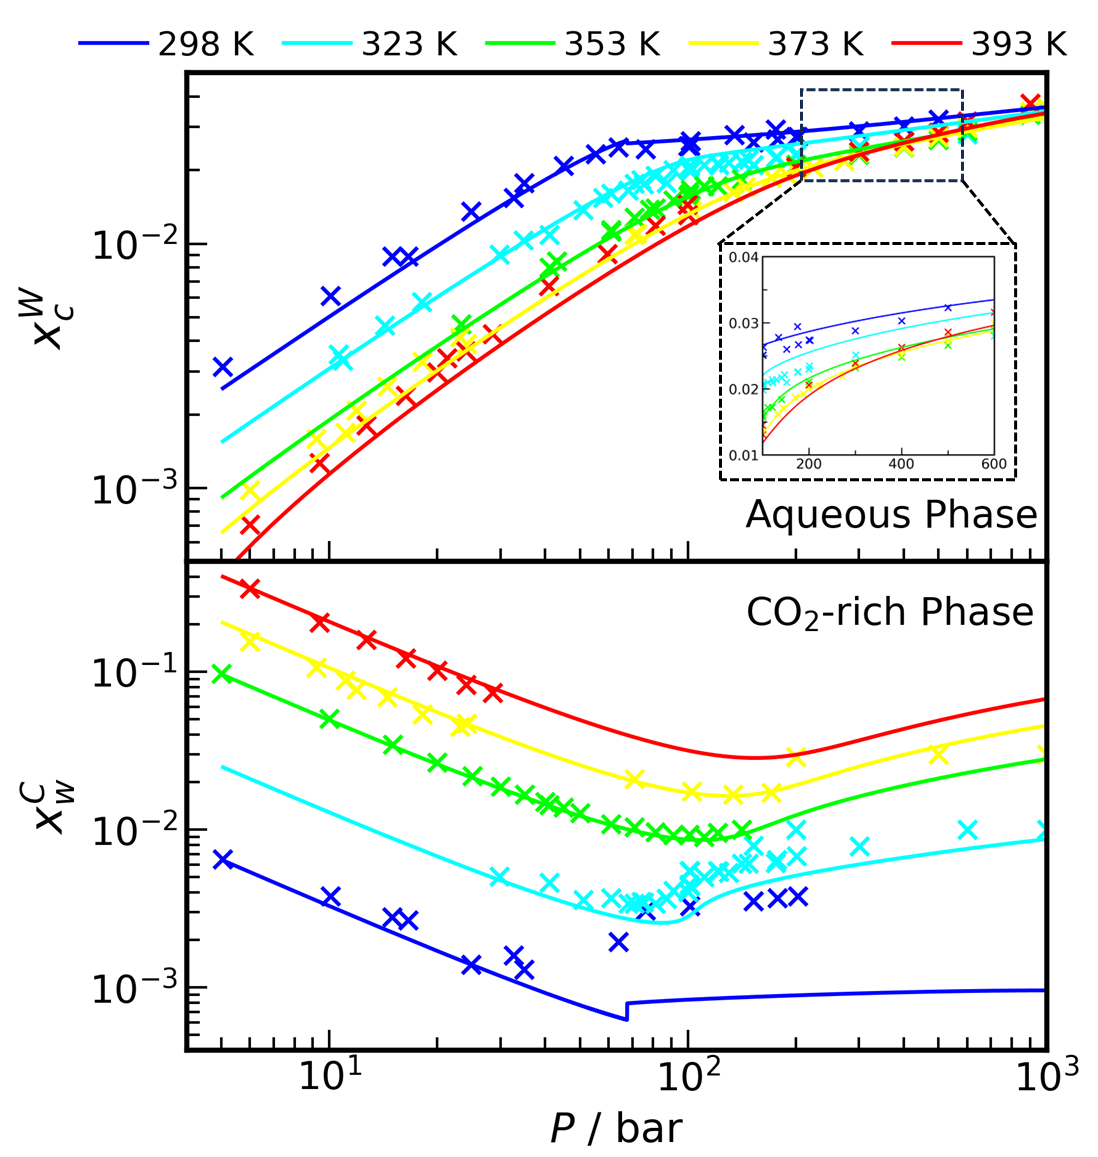
\includegraphics[width=0.65\textwidth]{Figures/ELV_CW_TLow.png} 
\caption{\ce{CO2} solubility in the aqueous phase (upper plot) and water solubility in the \ce{CO2}-rich phase (lower plot) \textit{vs.} pressure at low temperature ($T$ < 400 K) in the \ce{CO2}-water mixture from CPA EoS (continuous line) and experiments \cite{Guo2014, Valtz2004, Hou2013, King1992, Briones1987, Bamberger2000, Rumpf1994, Dsouza1988, Tödheide1963, Dohrn1993, Meyer2015, Nighswander1989, Tong2013} (discrete points).} 
\label{ELV_CW_Tlow}
\end{figure}

\newpage

\begin{figure}[h!]
\centering
  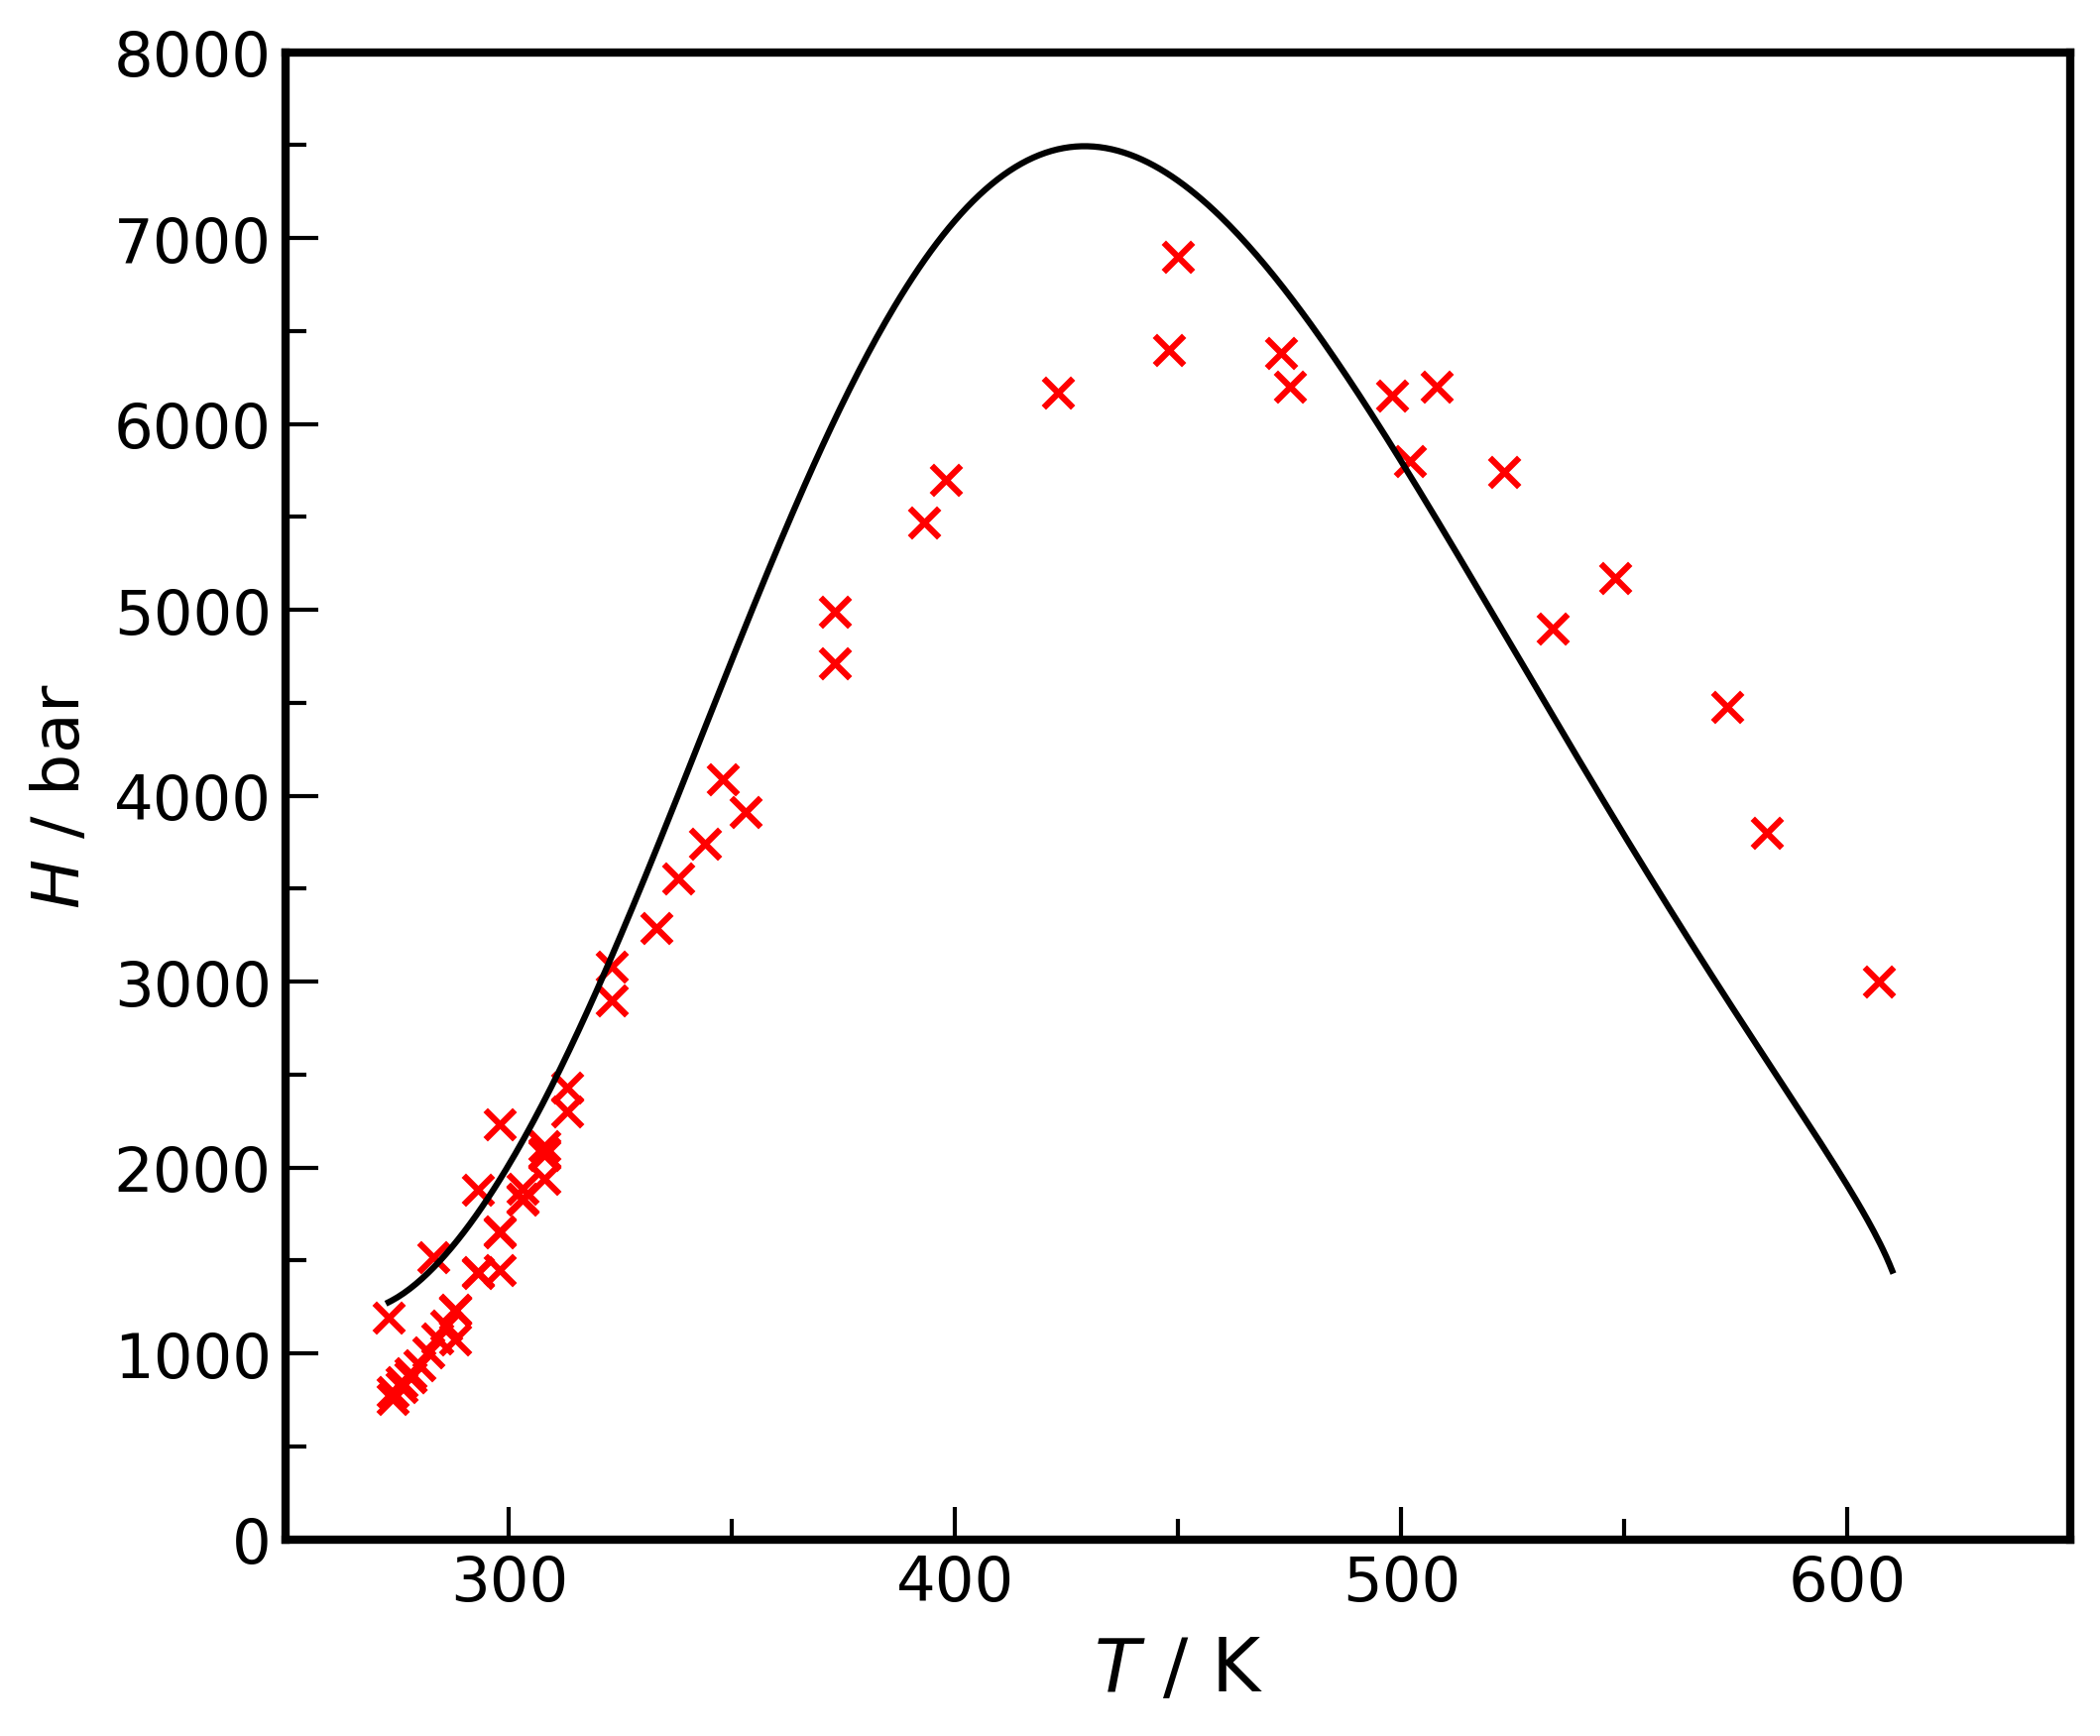
\includegraphics[width=0.7\textwidth]{Figures/HENRY.png} 
\caption{\ce{CO2} Henry's constant ($H$) in water \textit{vs.} temperature from CPA EoS (continuous line) and experiments \cite{Postigo1987, Tokunaga1975, Su2009, Schulze1981, Zheng1997, Dhima1999, Kiepe2002, Anderson2002, Malegaonkar1997, Dalmolin2006, Ellis1963} (discrete points).} 
\label{Henry}
\end{figure}


\newpage

\begin{figure}[h!]
\begin{subfigure}{.33\textwidth}
  \centering
  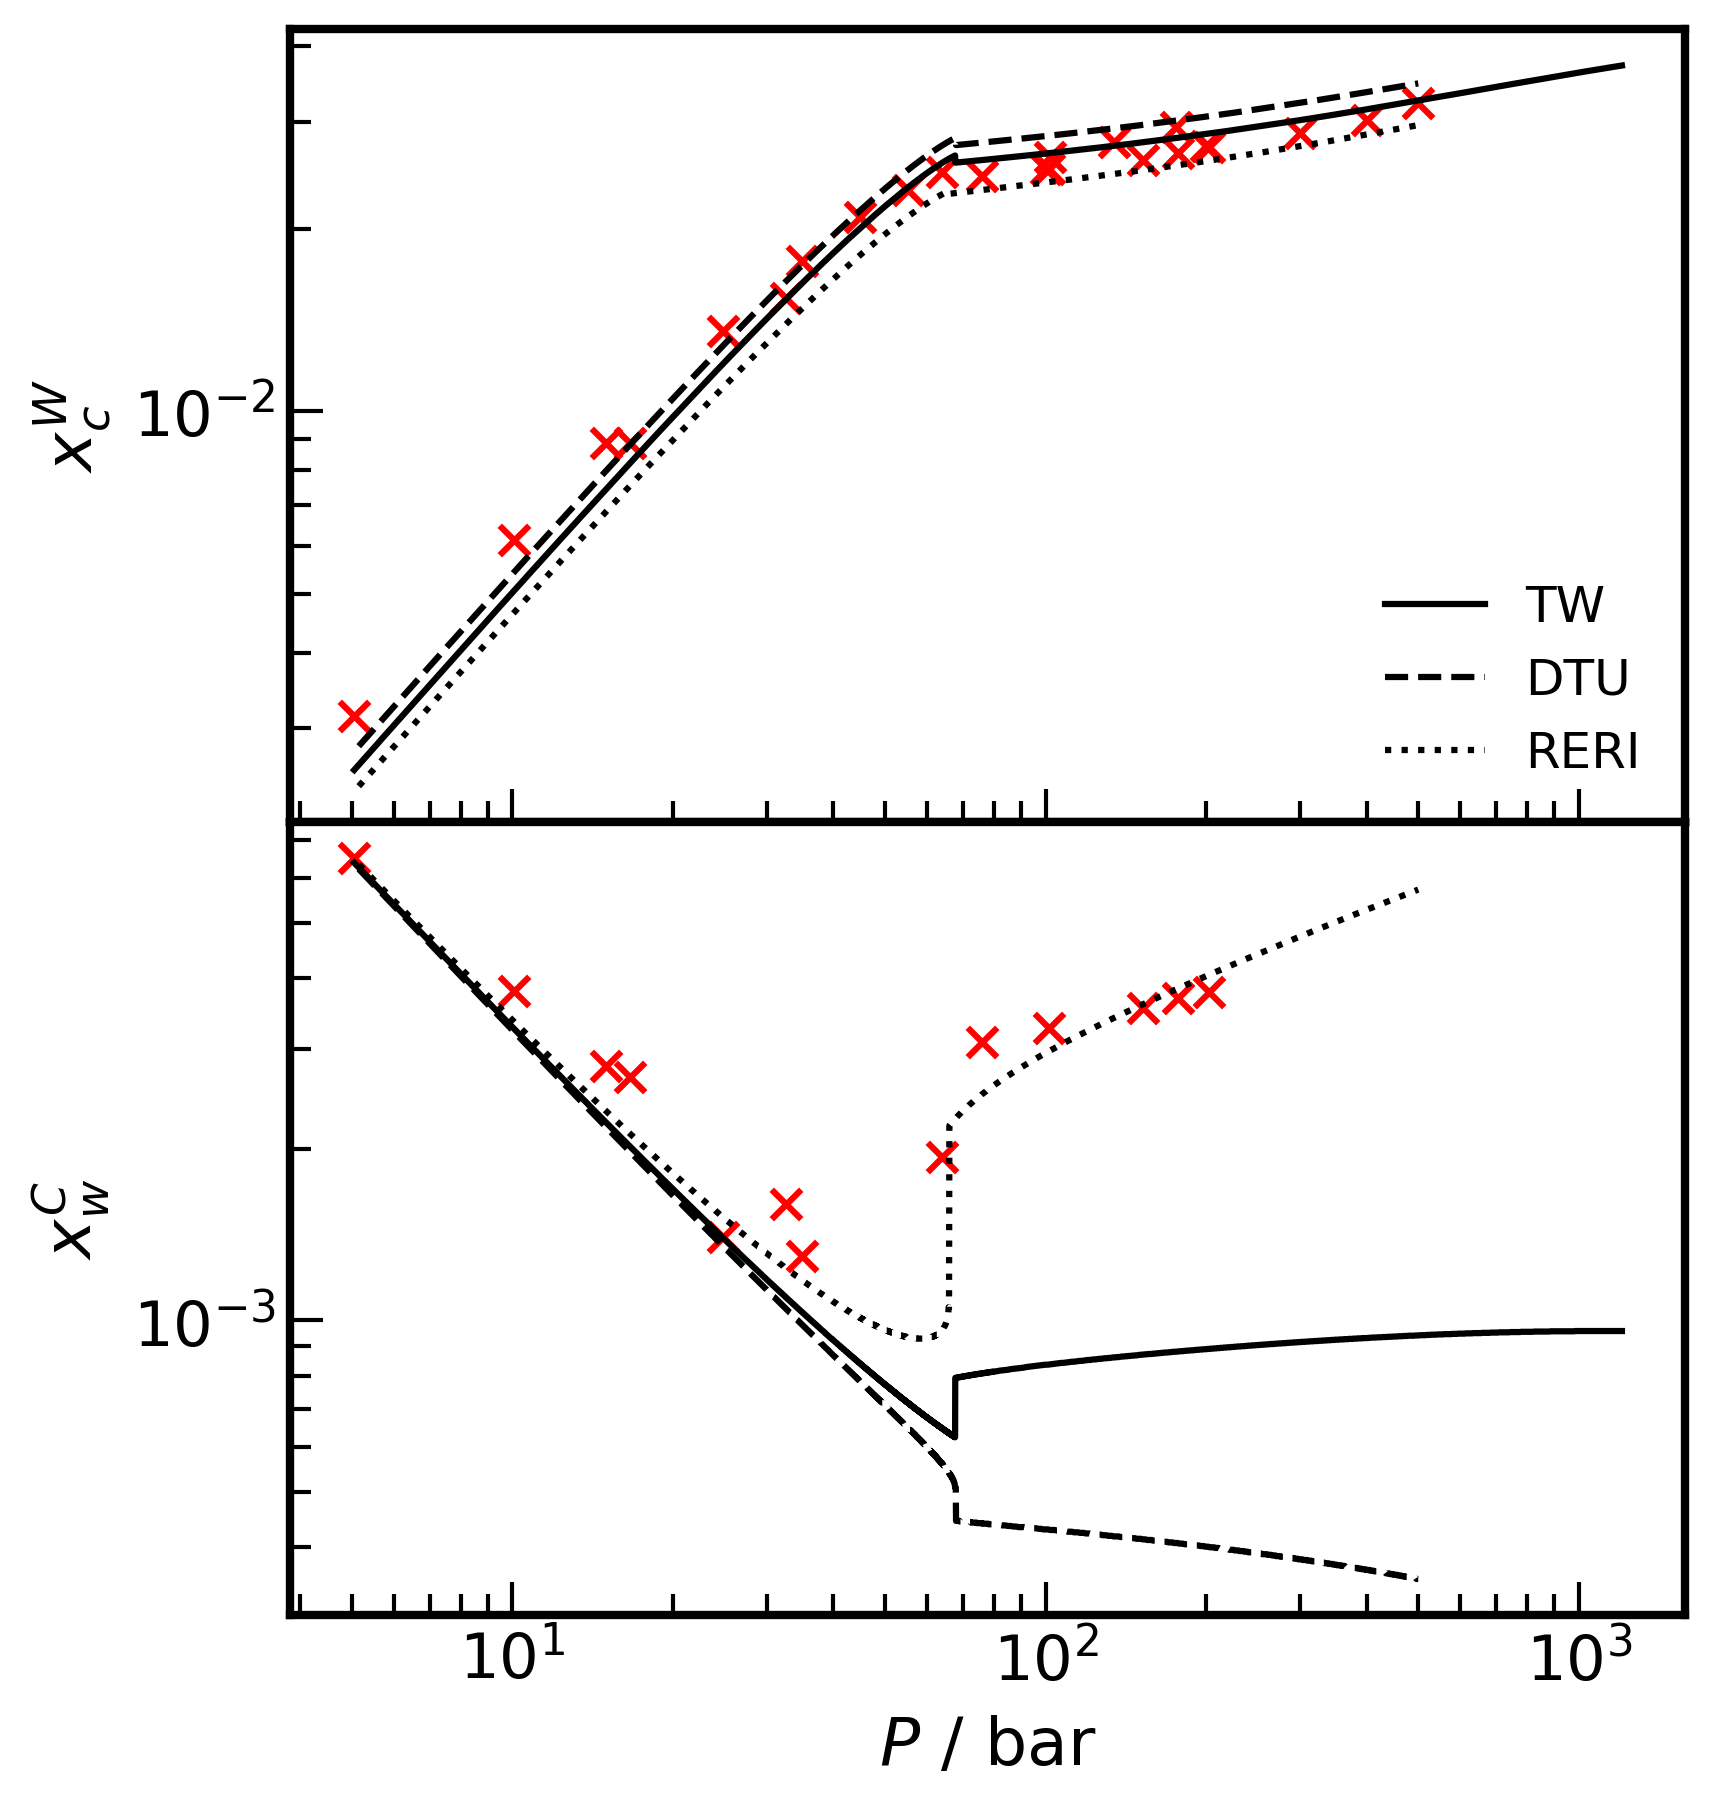
\includegraphics[width=.98\linewidth]{Figures/CPAmodels_T298K.png}
  \caption{$T$ = 298 K}
\end{subfigure}%
\begin{subfigure}{.33\textwidth}
  \centering
  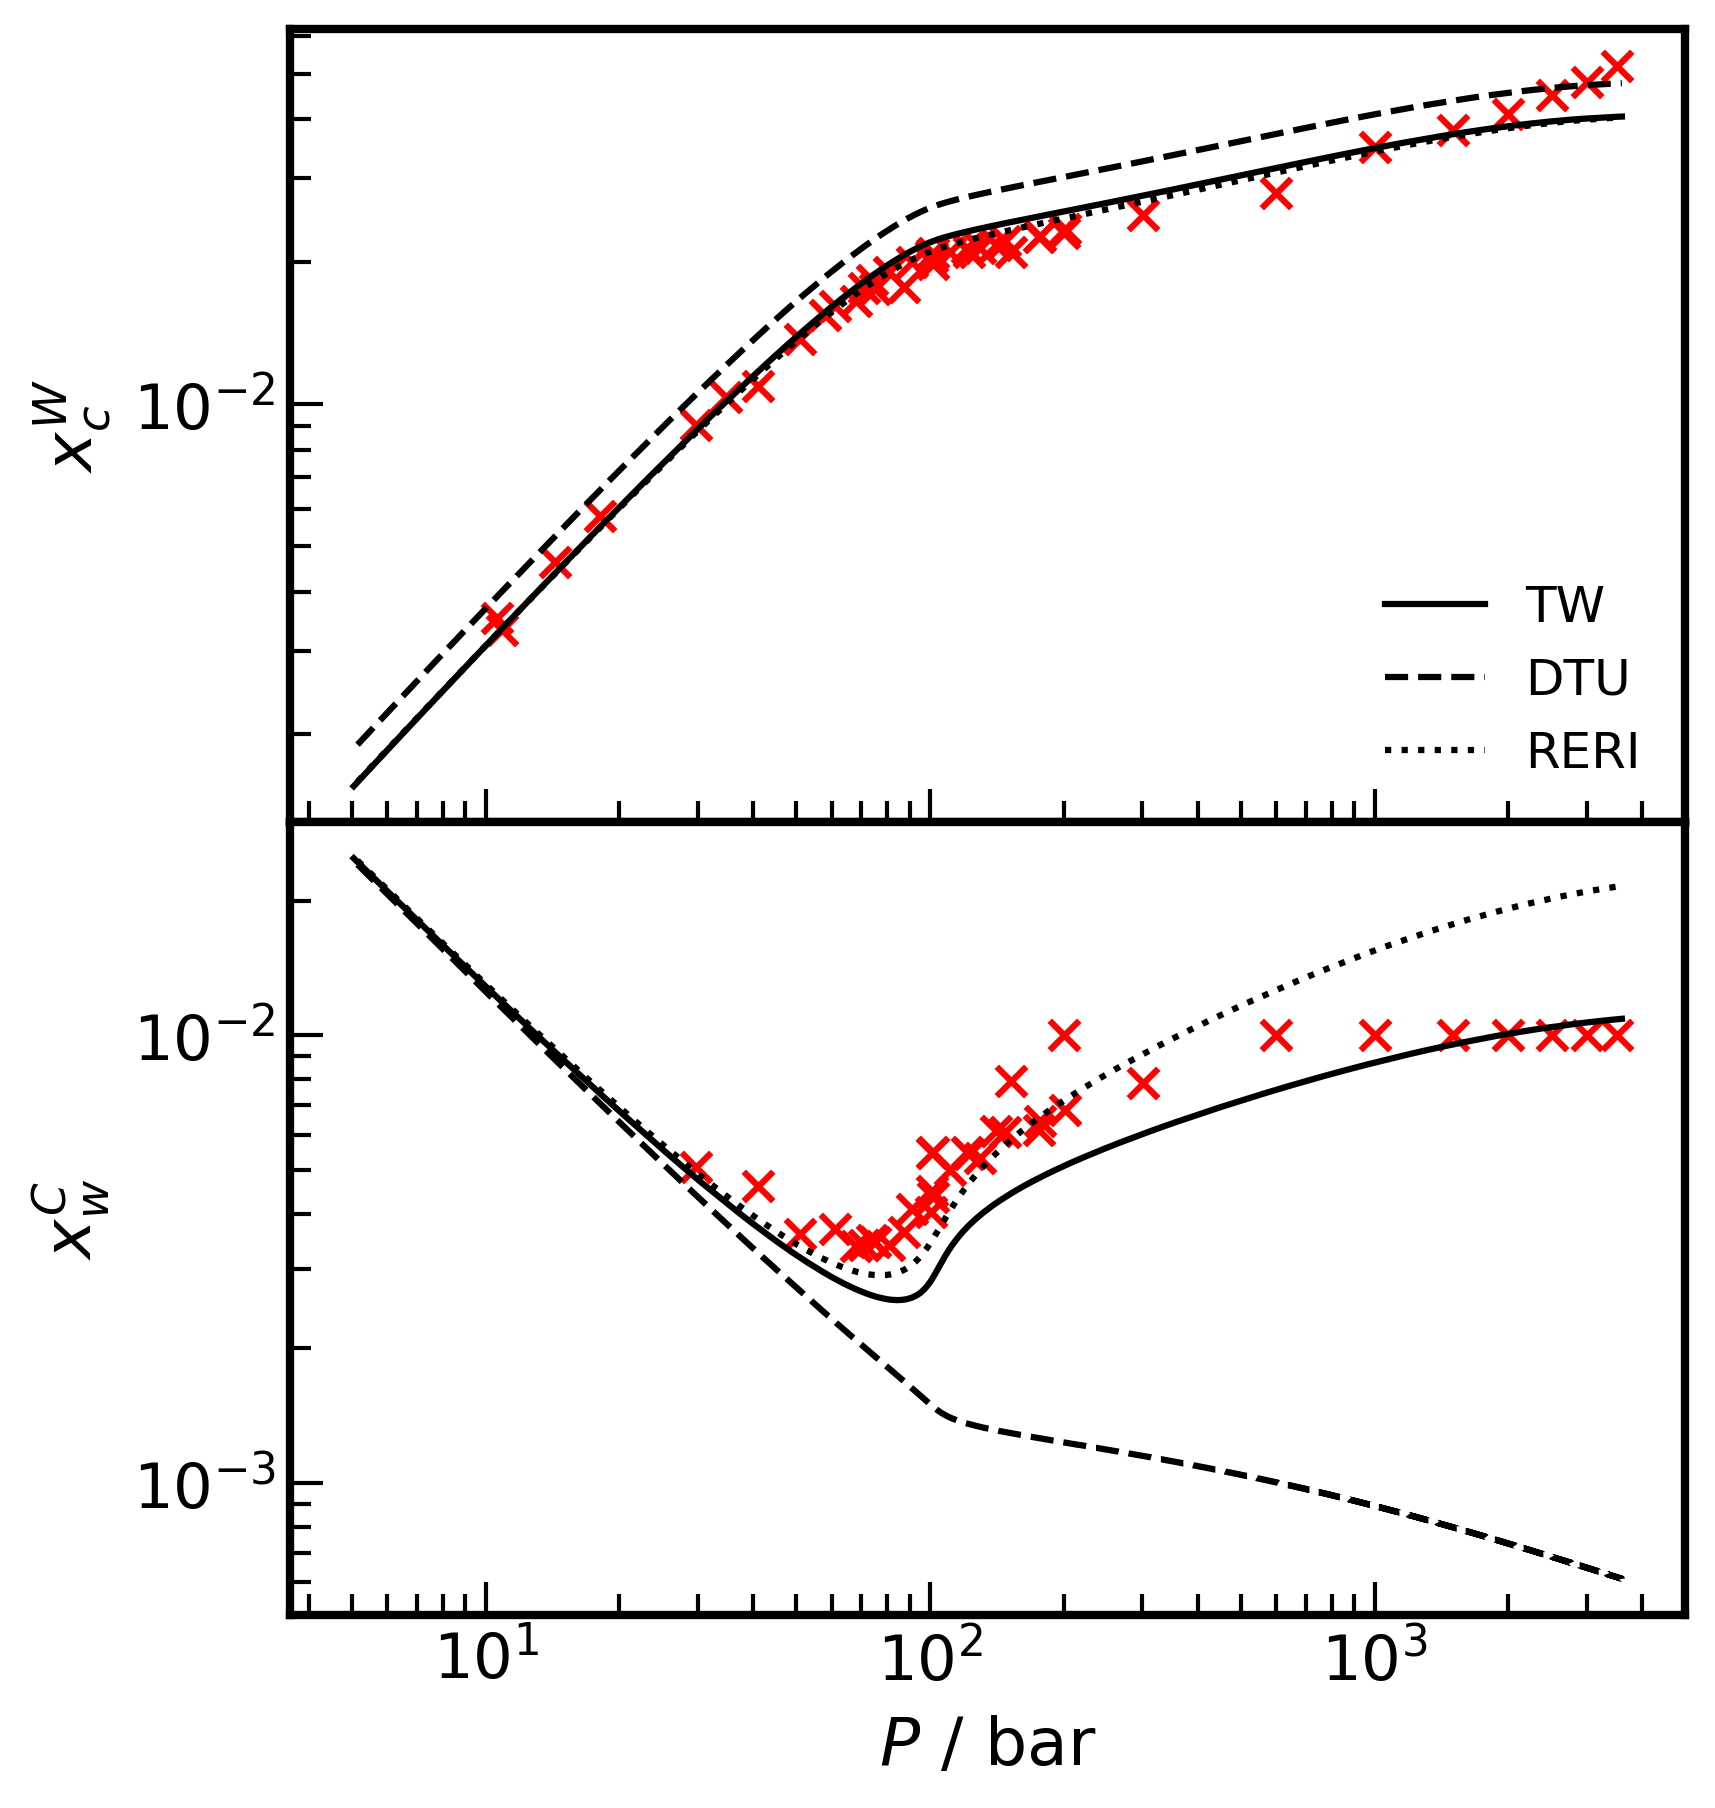
\includegraphics[width=.98\linewidth]{Figures/CPAmodels_T323K.png}
  \caption{$T$ = 323 K}
\end{subfigure}%
\begin{subfigure}{.33\textwidth}
  \centering
  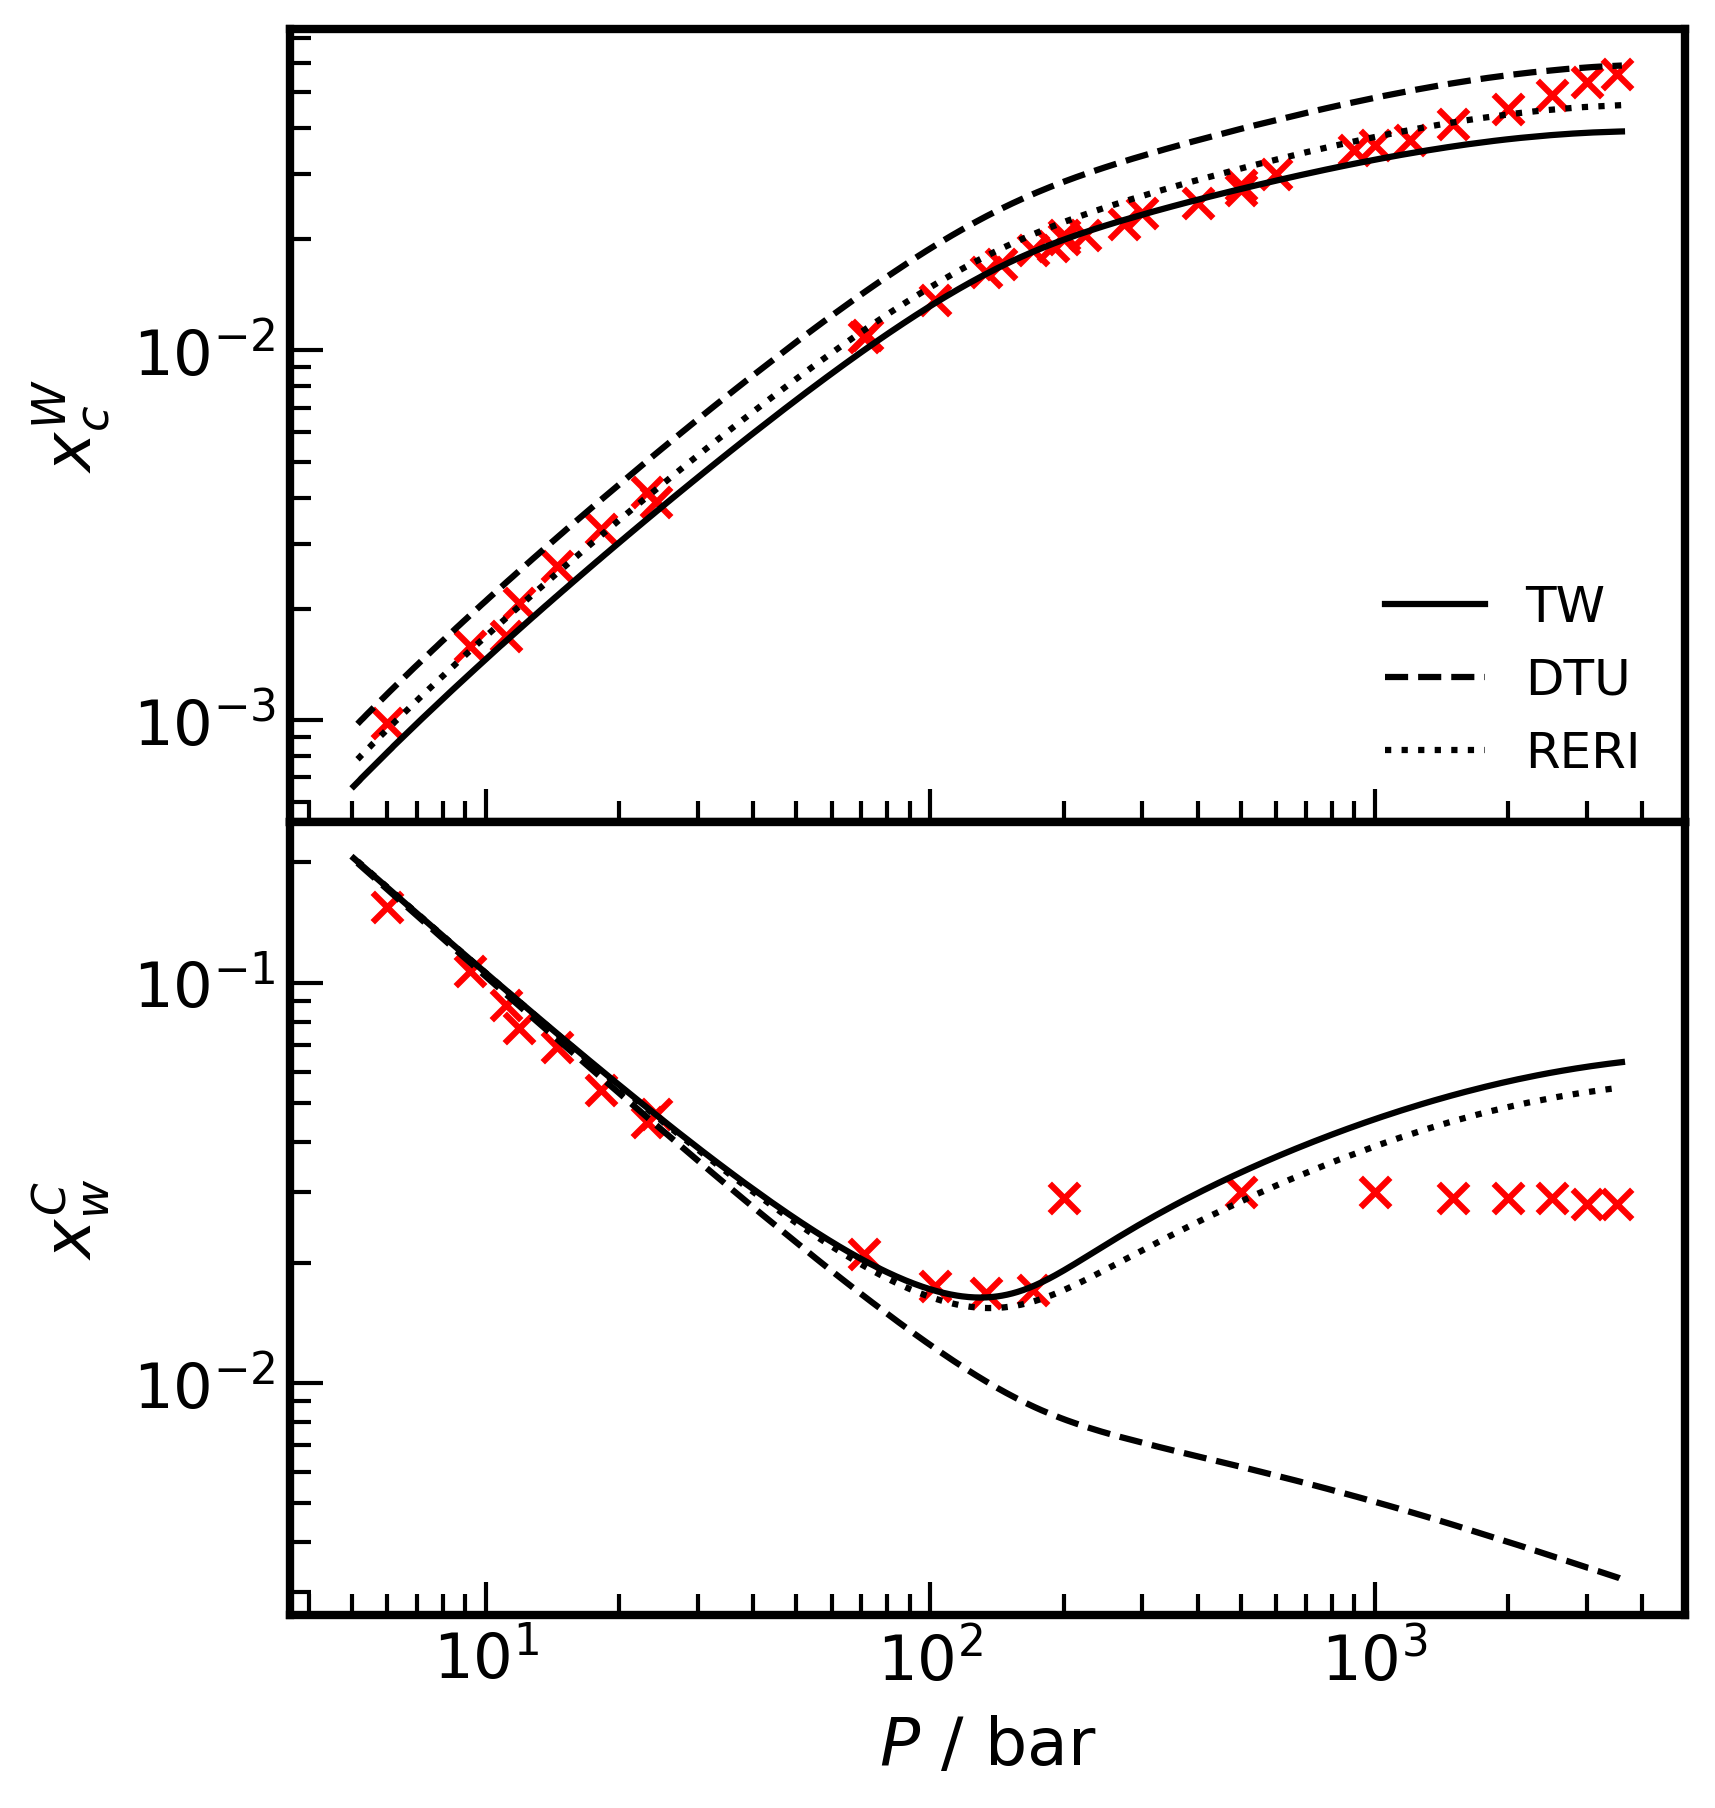
\includegraphics[width=.98\linewidth]{Figures/CPAmodels_T373K.png}
  \caption{$T$ = 373 K}
\end{subfigure}%
\vskip\baselineskip
\begin{subfigure}{.33\textwidth}
  \centering
  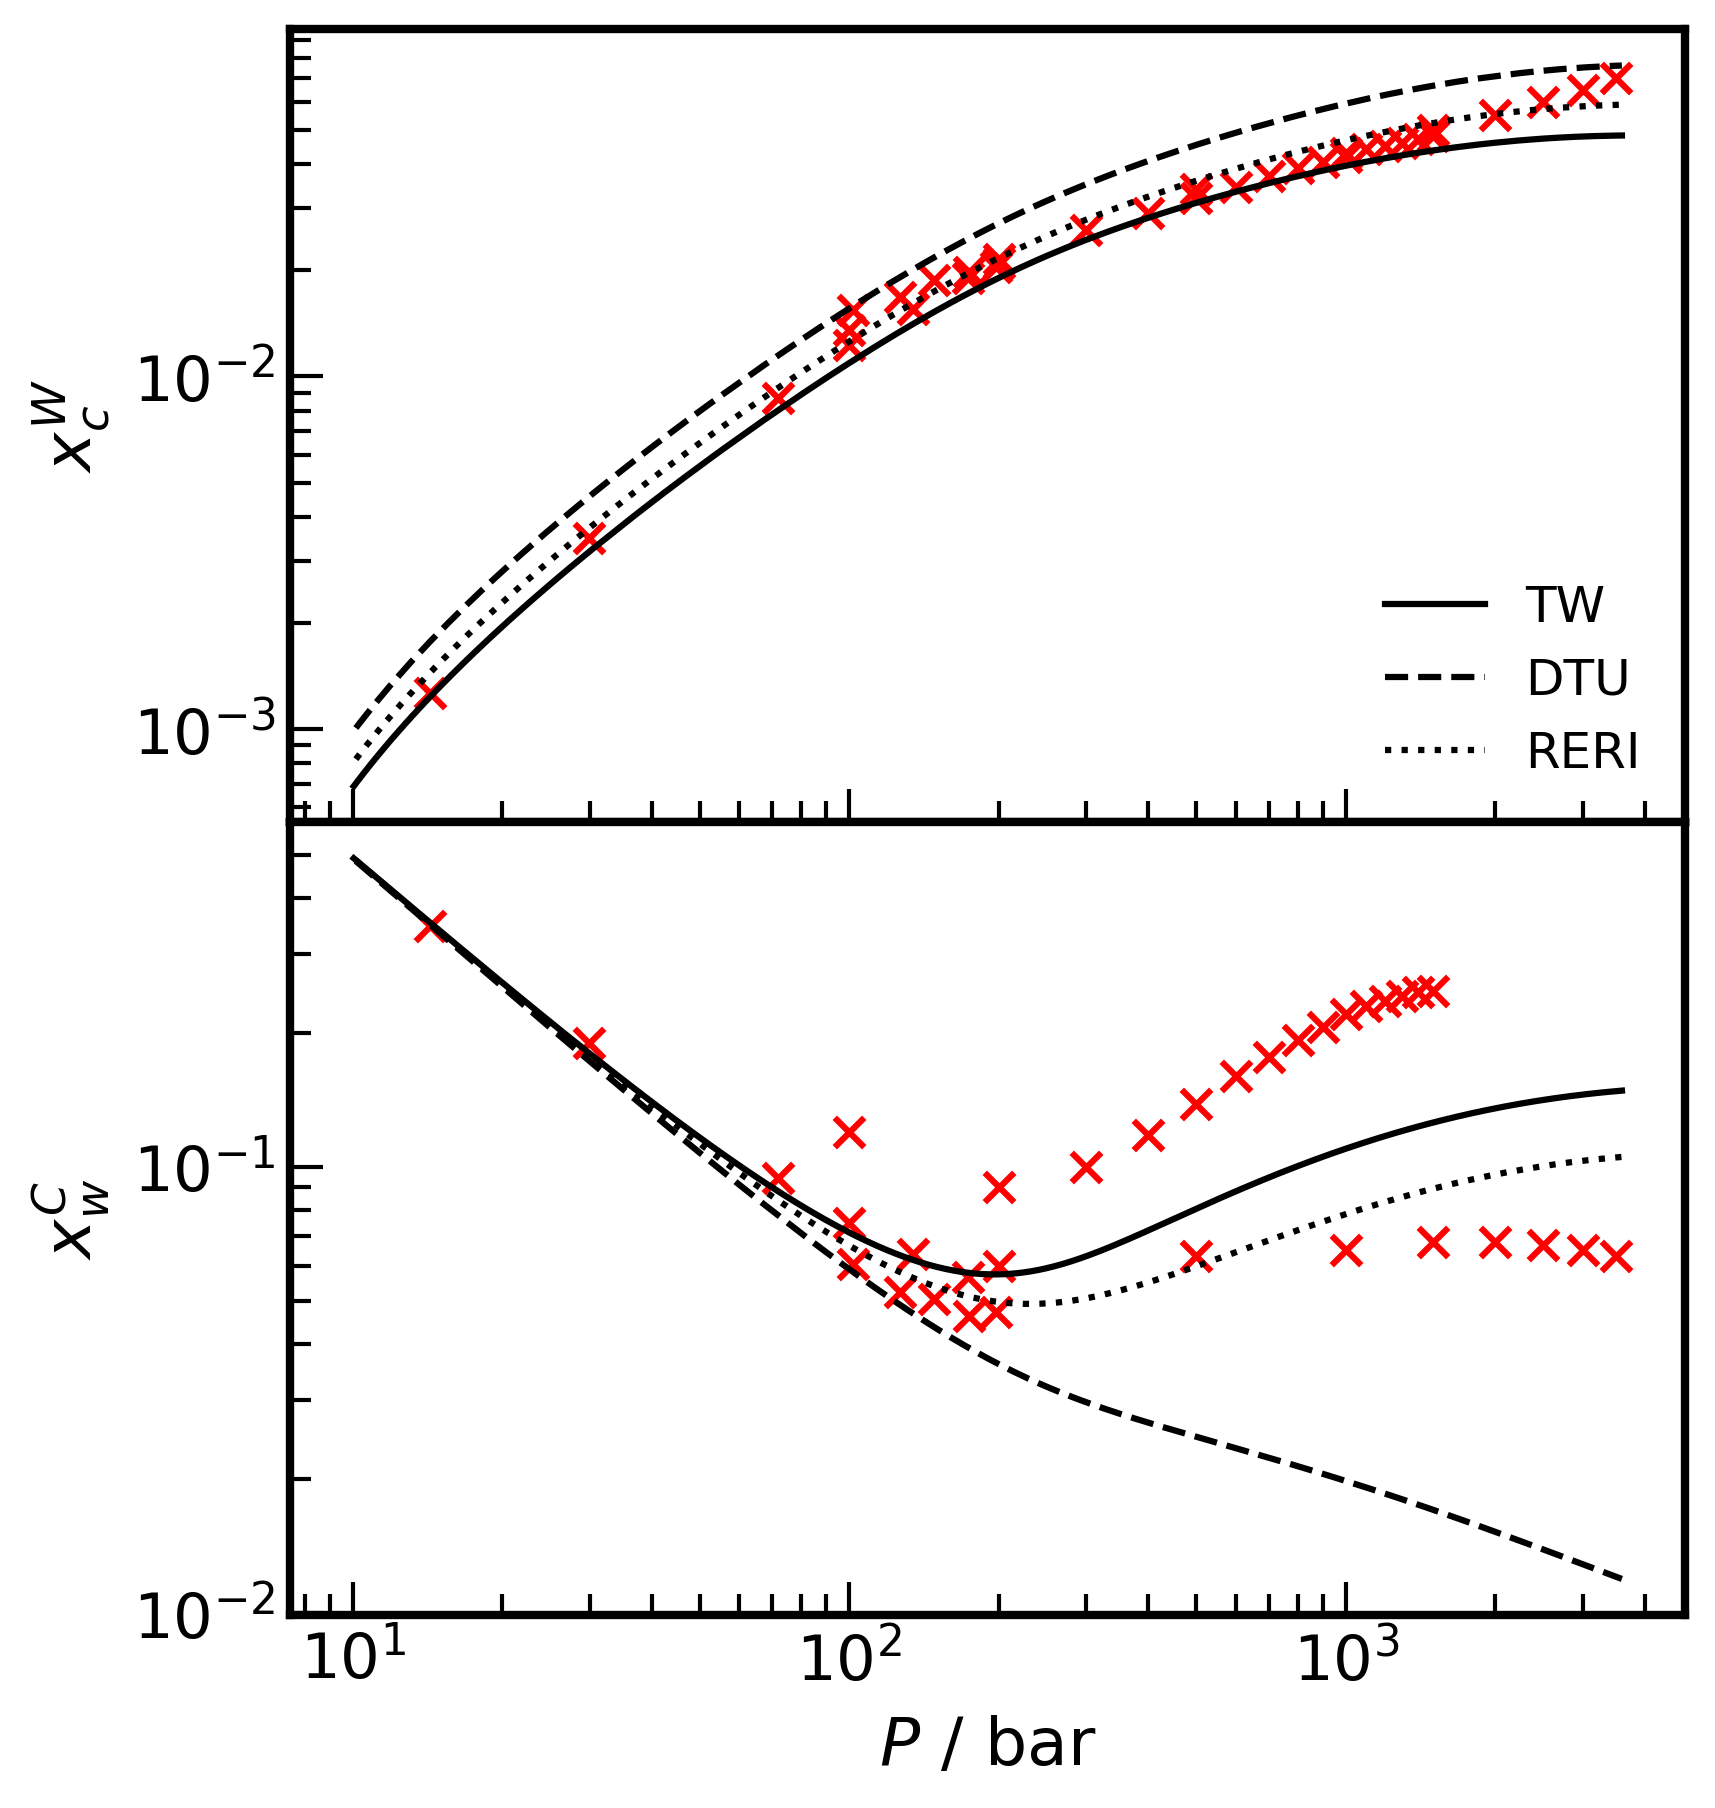
\includegraphics[width=.98\linewidth]{Figures/CPAmodels_T423K.png}
  \caption{$T$ = 423 K}
\end{subfigure}%
\begin{subfigure}{.33\textwidth}
  \centering
  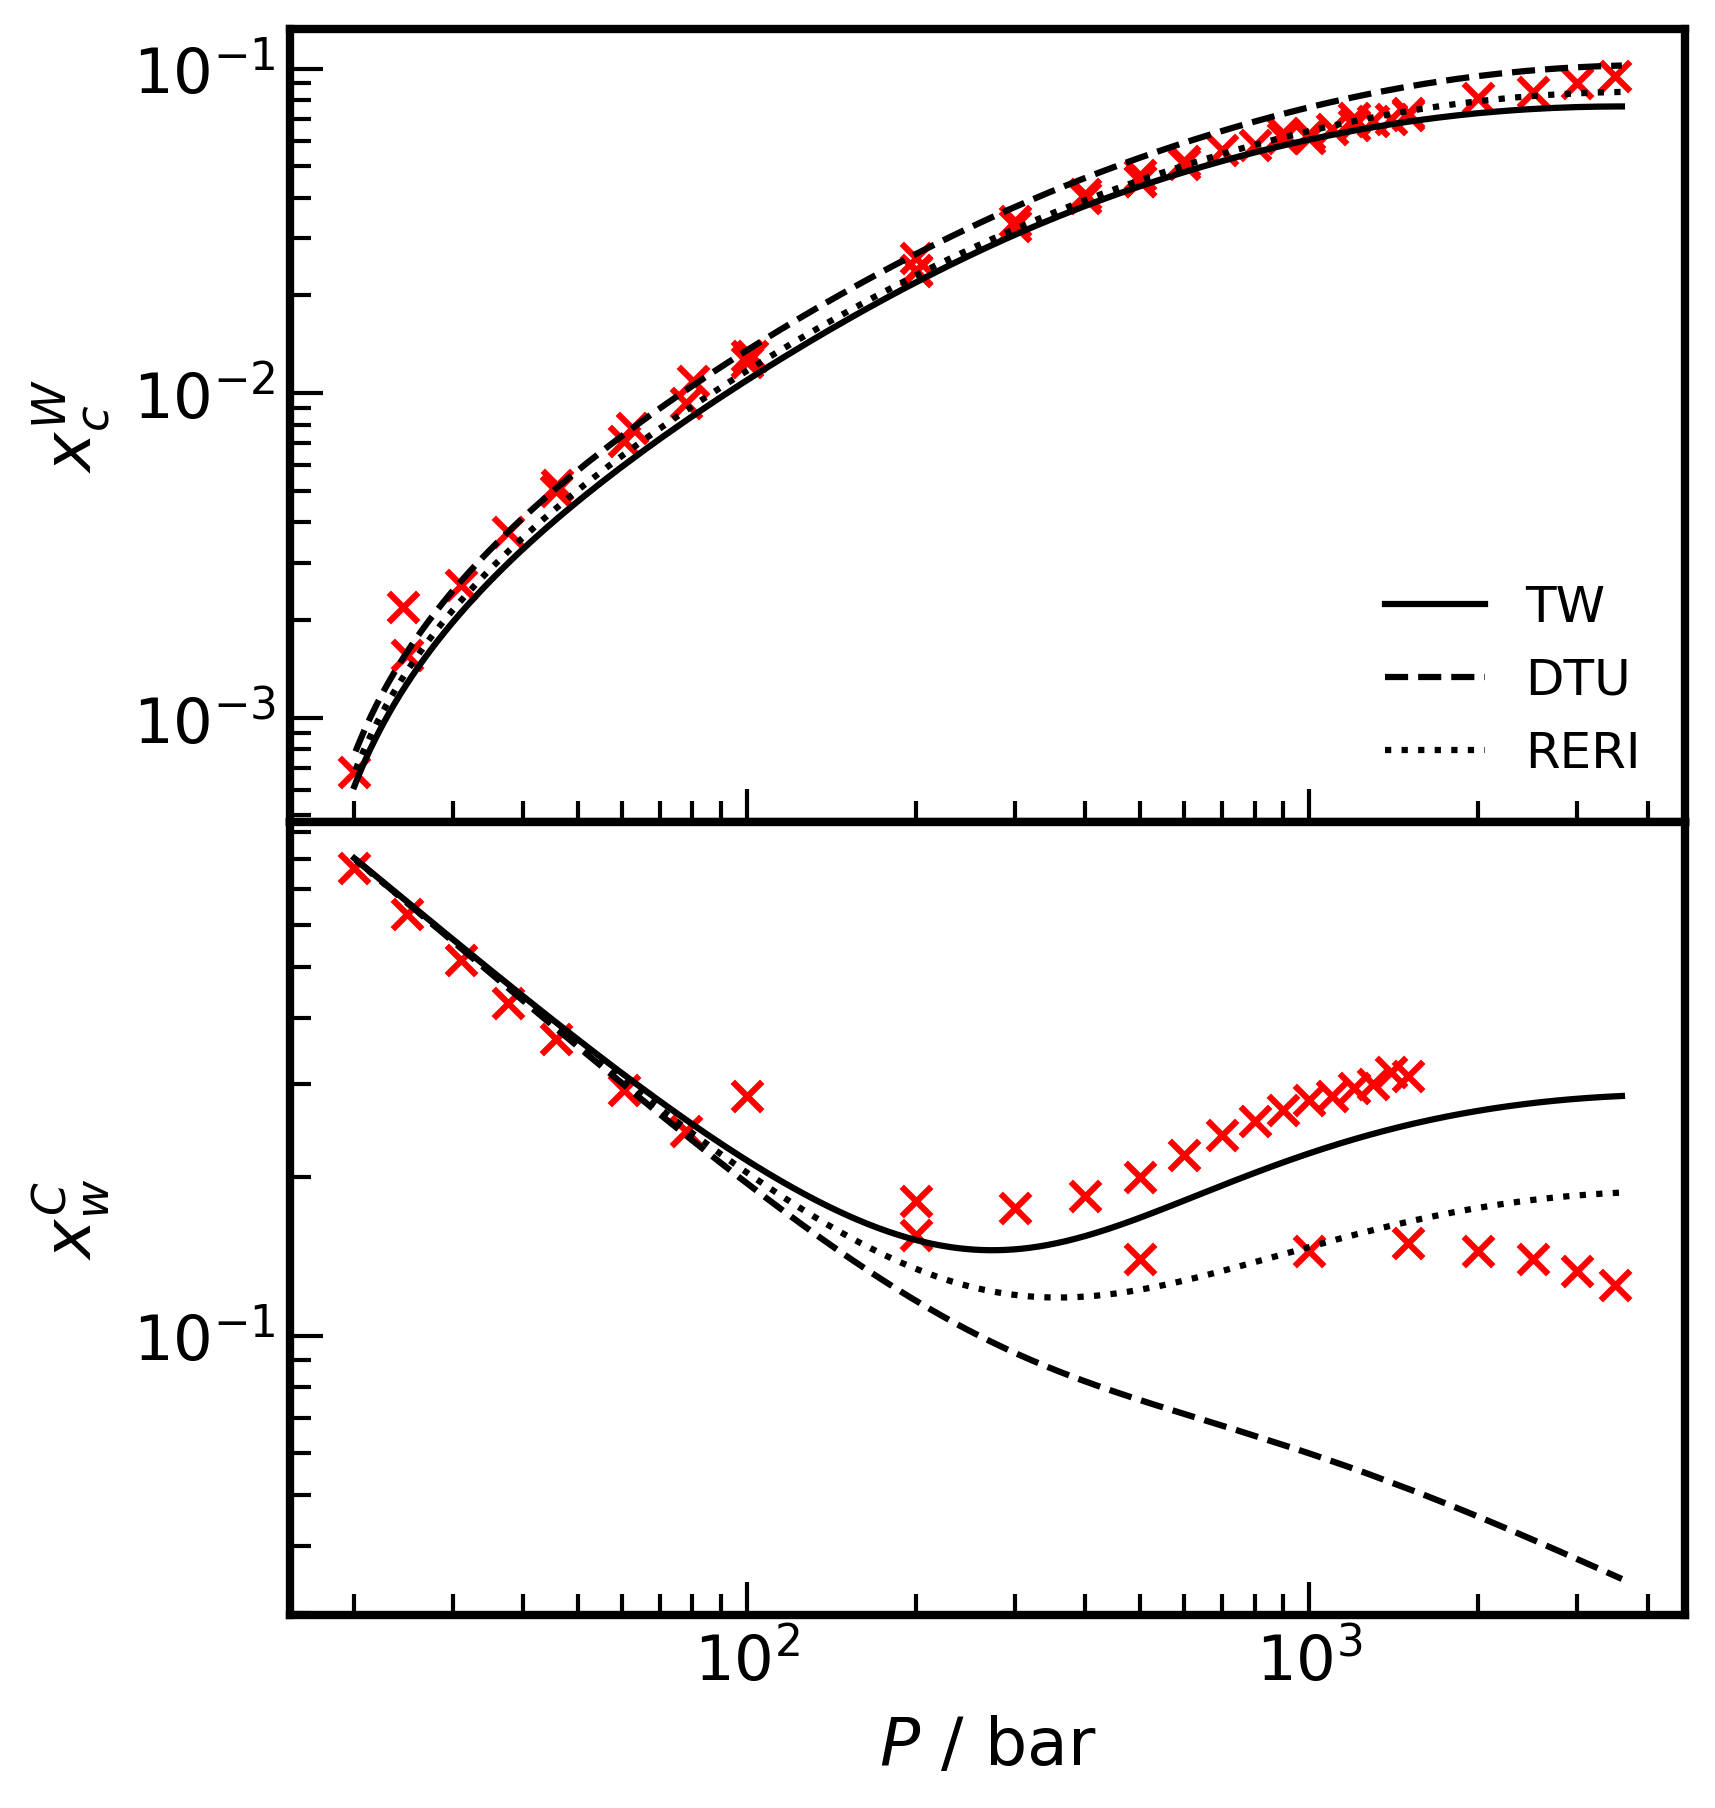
\includegraphics[width=.98\linewidth]{Figures/CPAmodels_T473K.png}
  \caption{$T$ = 473 K}
\end{subfigure}%
\begin{subfigure}{.33\textwidth}
  \centering
  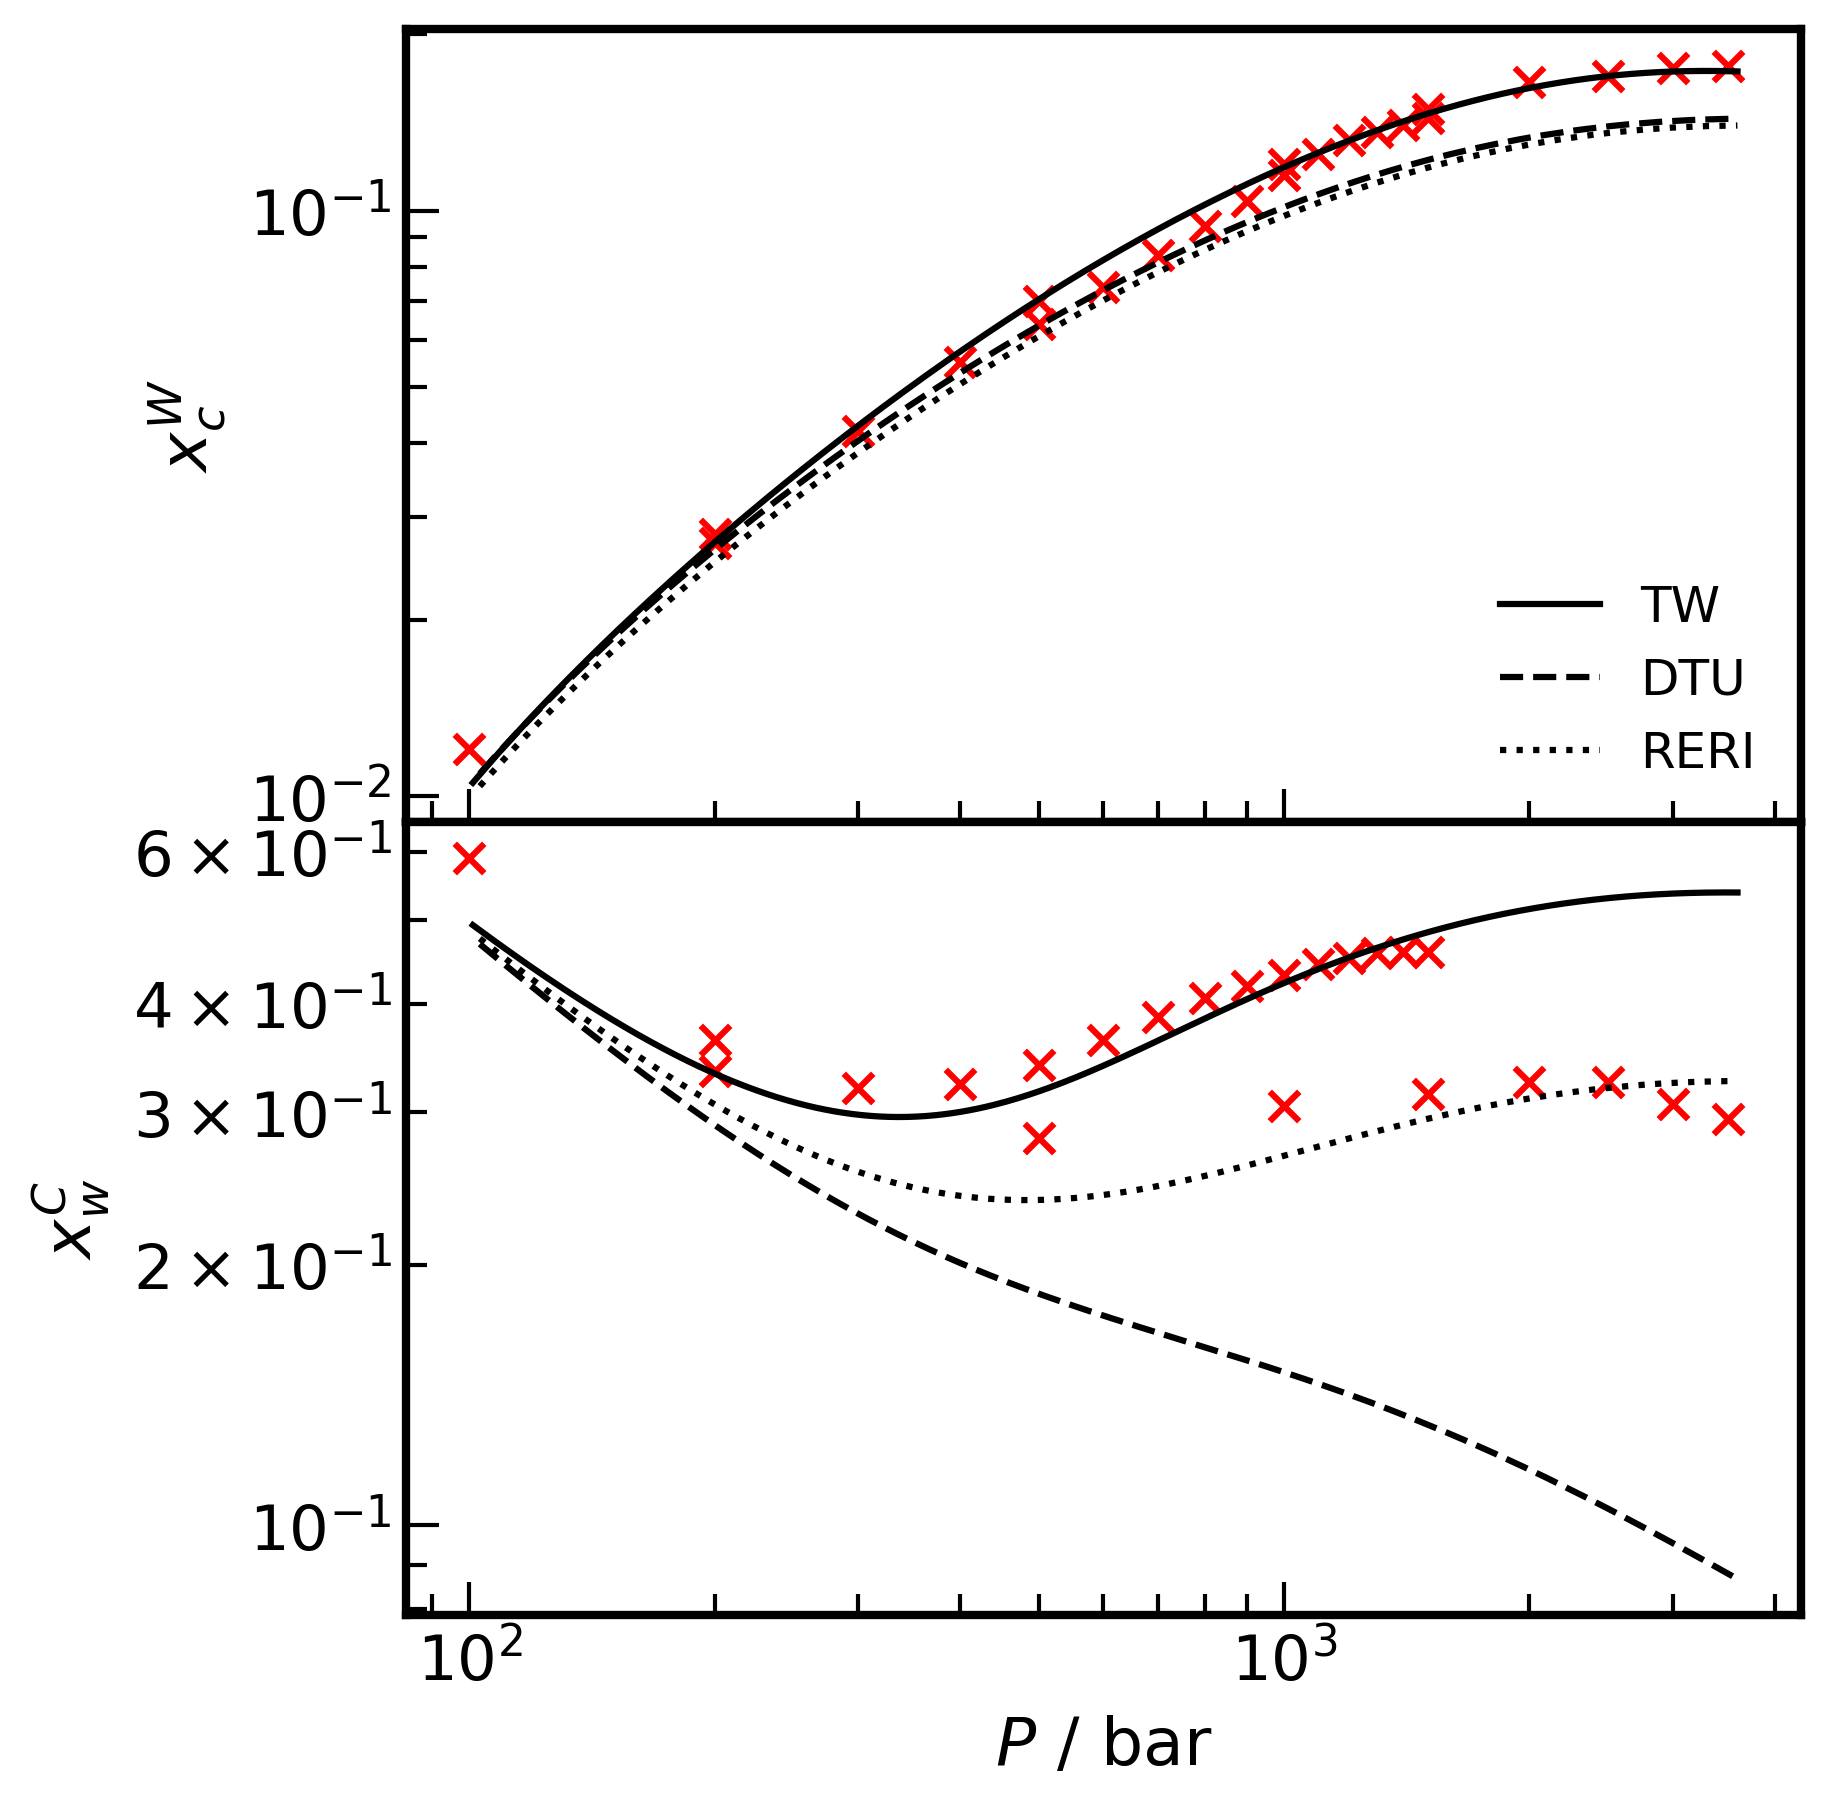
\includegraphics[width=.98\linewidth]{Figures/CPAmodels_T523K.png}
  \caption{$T$ = 523 K}
\end{subfigure}%
\label{TW_DTU_RERI1}
\caption{\ce{CO2} solubility in the aqueous phase (upper plot) and water solubility in the \ce{CO2}-rich phase (lower plot) \textit{vs.} pressure at various temperatures (a-f) from CPA EoS models (This Work (TW), DTU \cite{Tsivintzelis2011, Maribo2015, Olsen2021} and RERI \cite{Li2009}) and experiments \cite{Guo2014, Valtz2004, Hou2013, King1992, Briones1987, Bamberger2000, Rumpf1994, Dsouza1988, Tödheide1963, Dohrn1993, Meyer2015, Nighswander1989, Tong2013, Takenouchi1964, Sako1991, Muller1988} (discrete points).} 
\end{figure}

\newpage

\begin{figure}[h!]
\begin{subfigure}{.49\textwidth}
  \centering
  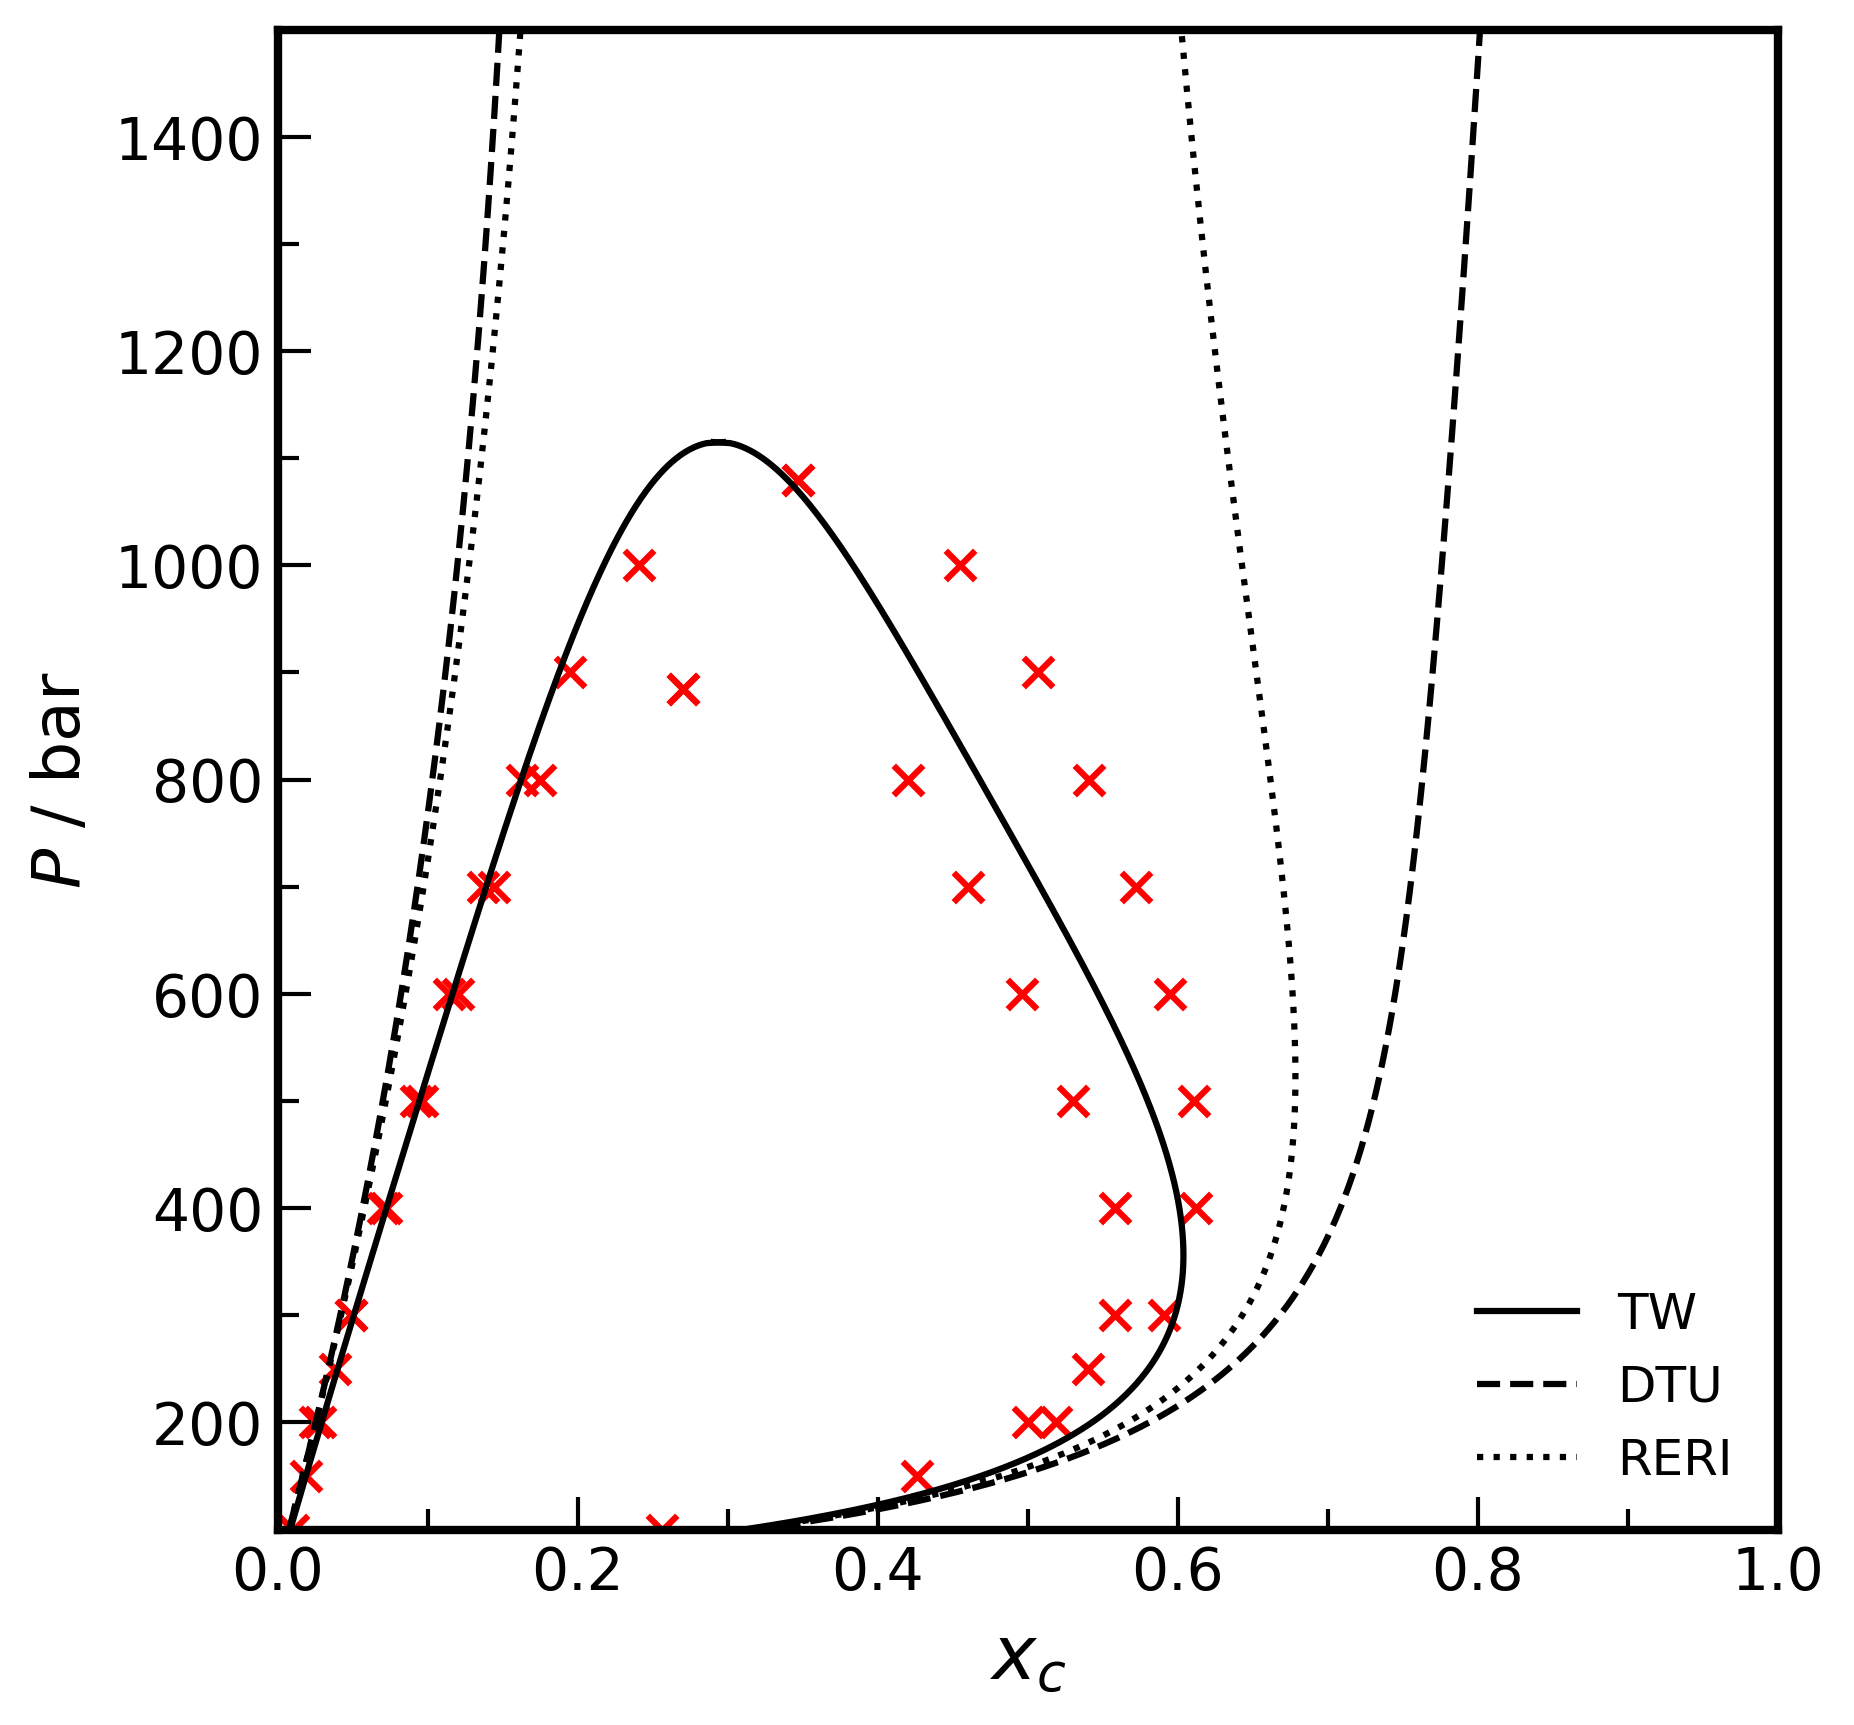
\includegraphics[width=.82\linewidth]{Figures/CPAmodels_T548K.png}
  \caption{$T$ = 548 K}
\end{subfigure}%
\begin{subfigure}{.49\textwidth}
  \centering
  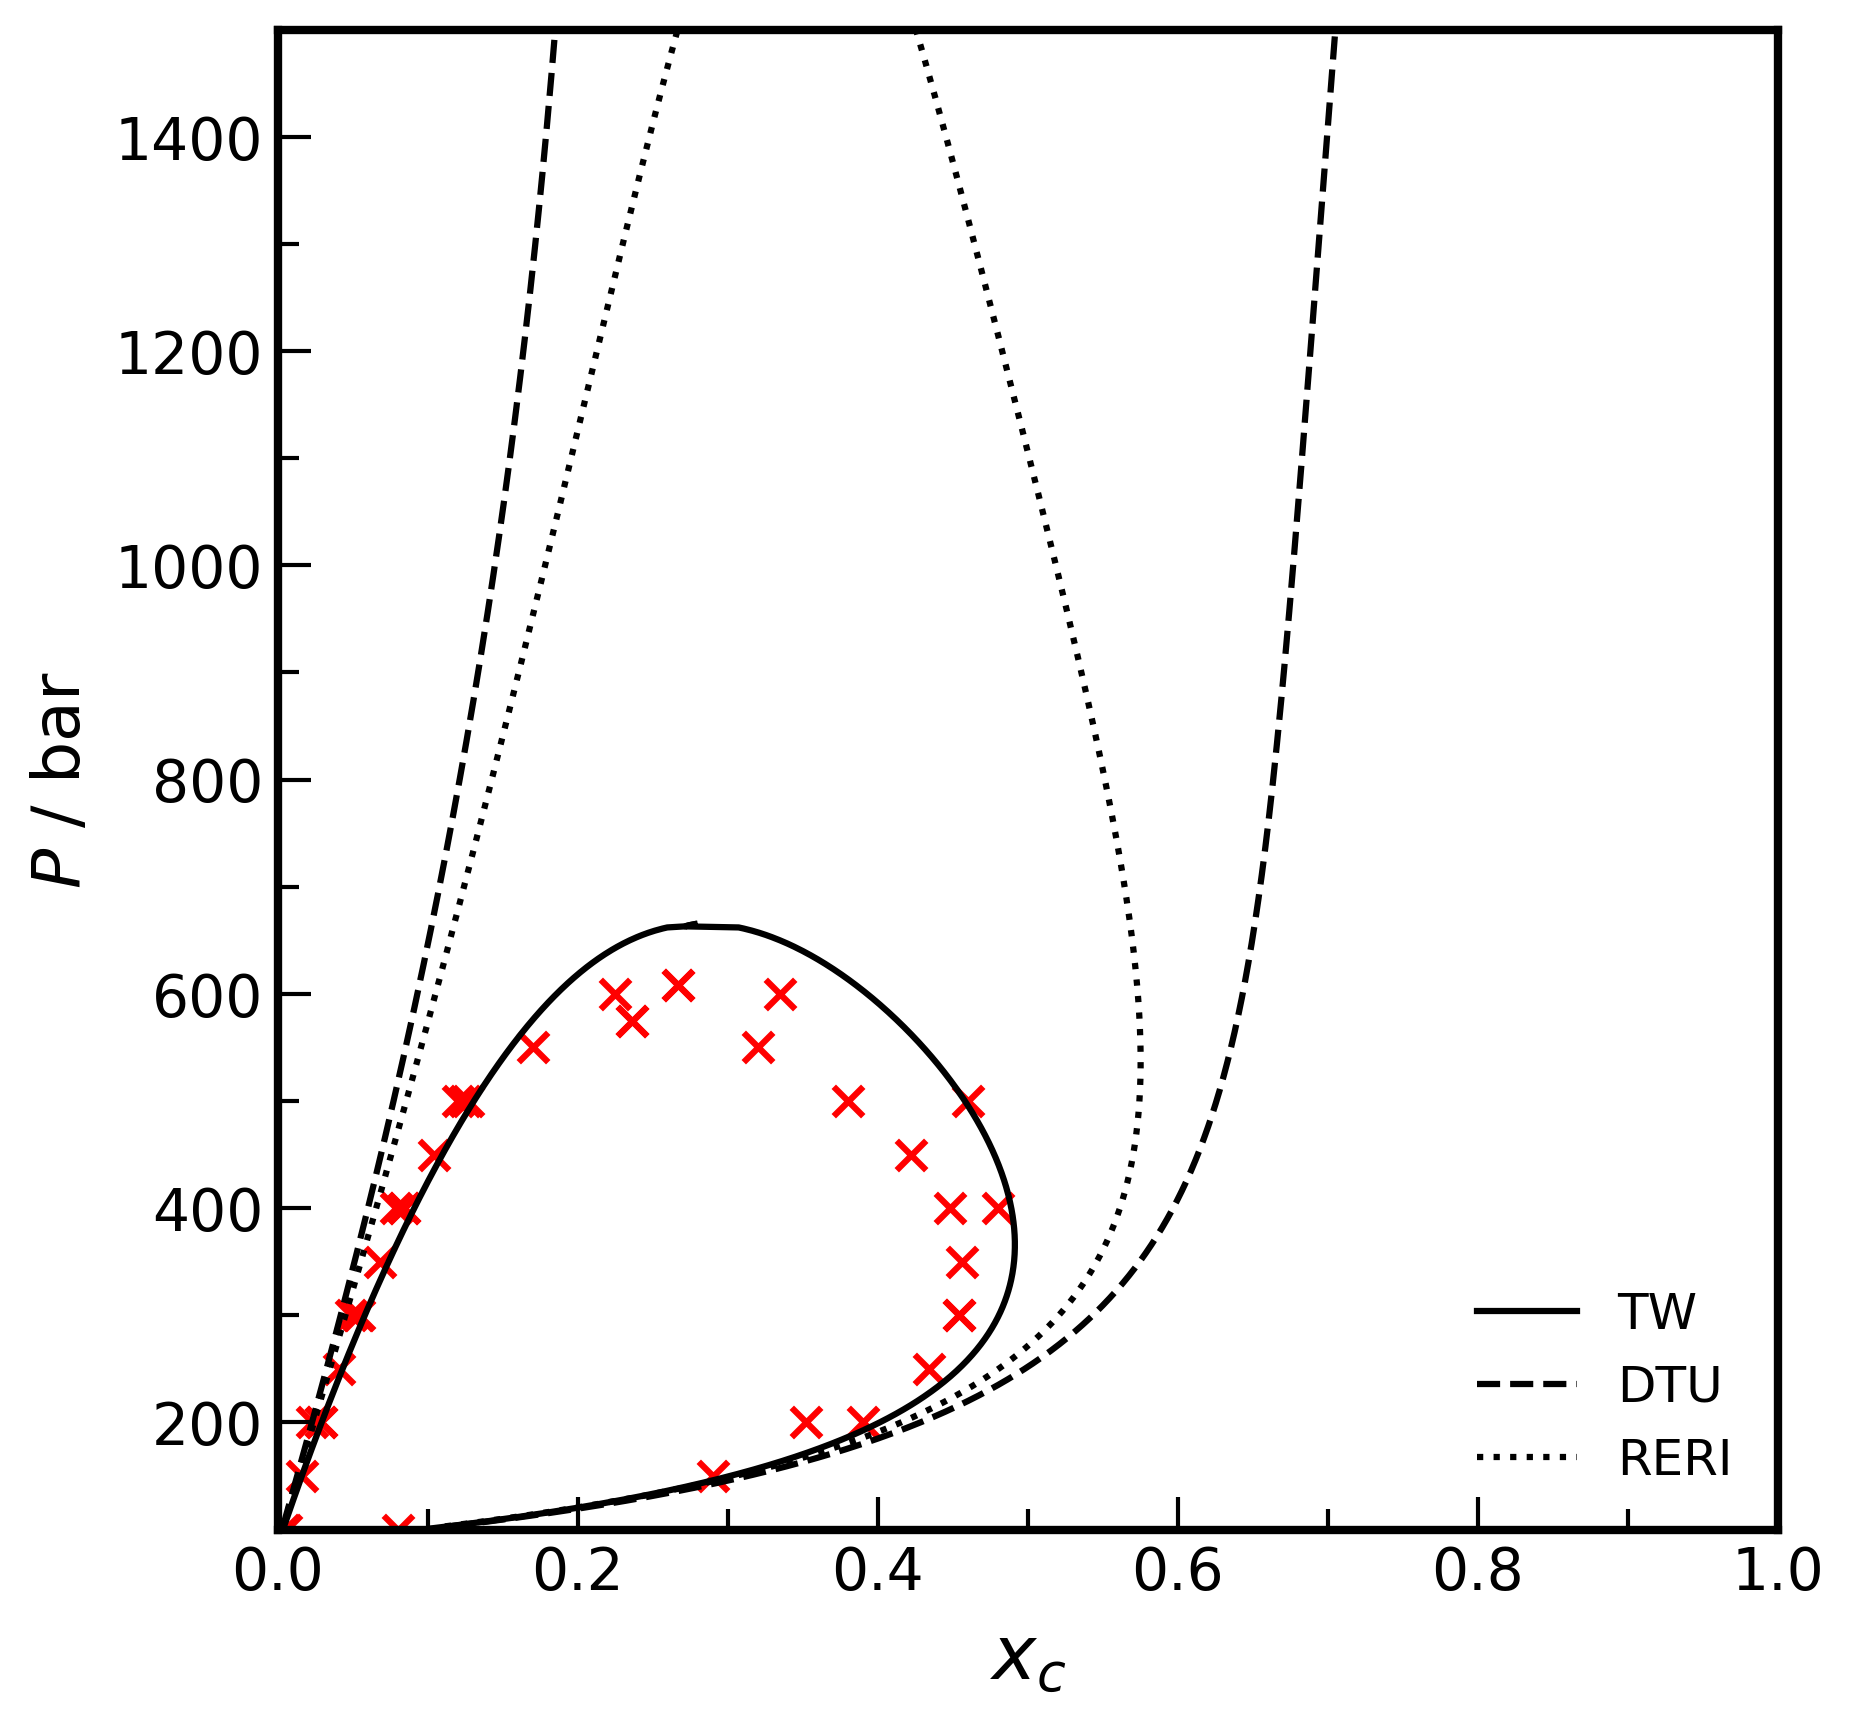
\includegraphics[width=.82\linewidth]{Figures/CPAmodels_T573K.png}
  \caption{$T$ = 573 K}
\end{subfigure}%
\vskip\baselineskip
\begin{subfigure}{.49\textwidth}
  \centering
  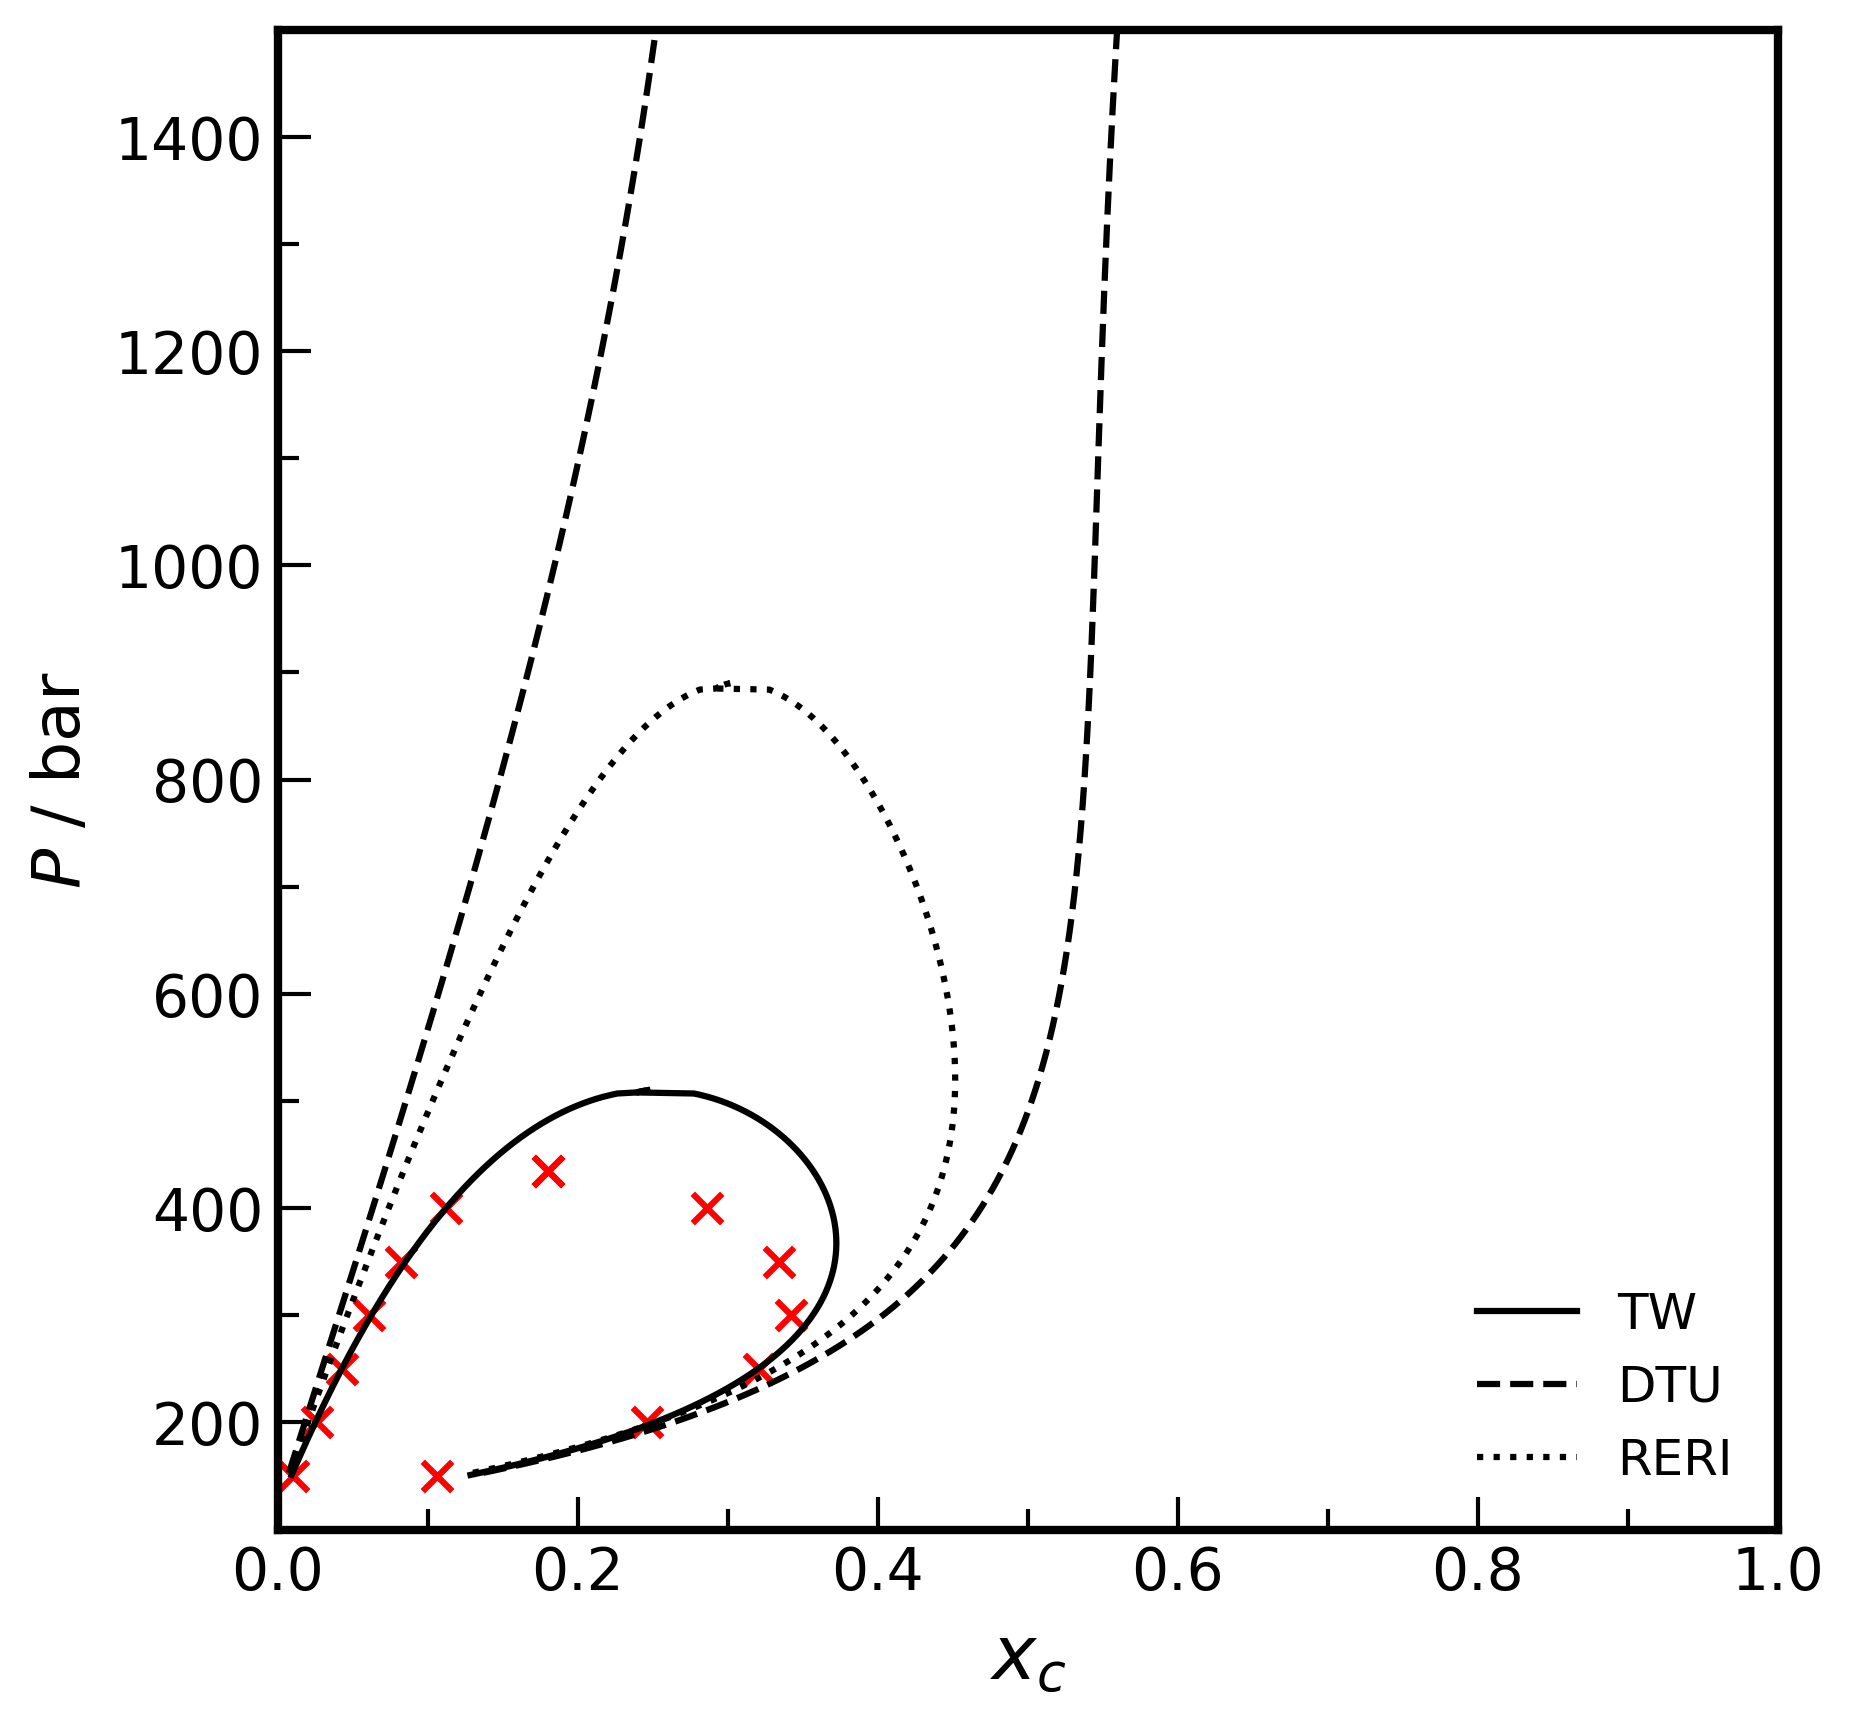
\includegraphics[width=.82\linewidth]{Figures/CPAmodels_T598K.png}
  \caption{$T$ = 598 K}
\end{subfigure}%
\begin{subfigure}{.49\textwidth}
  \centering
  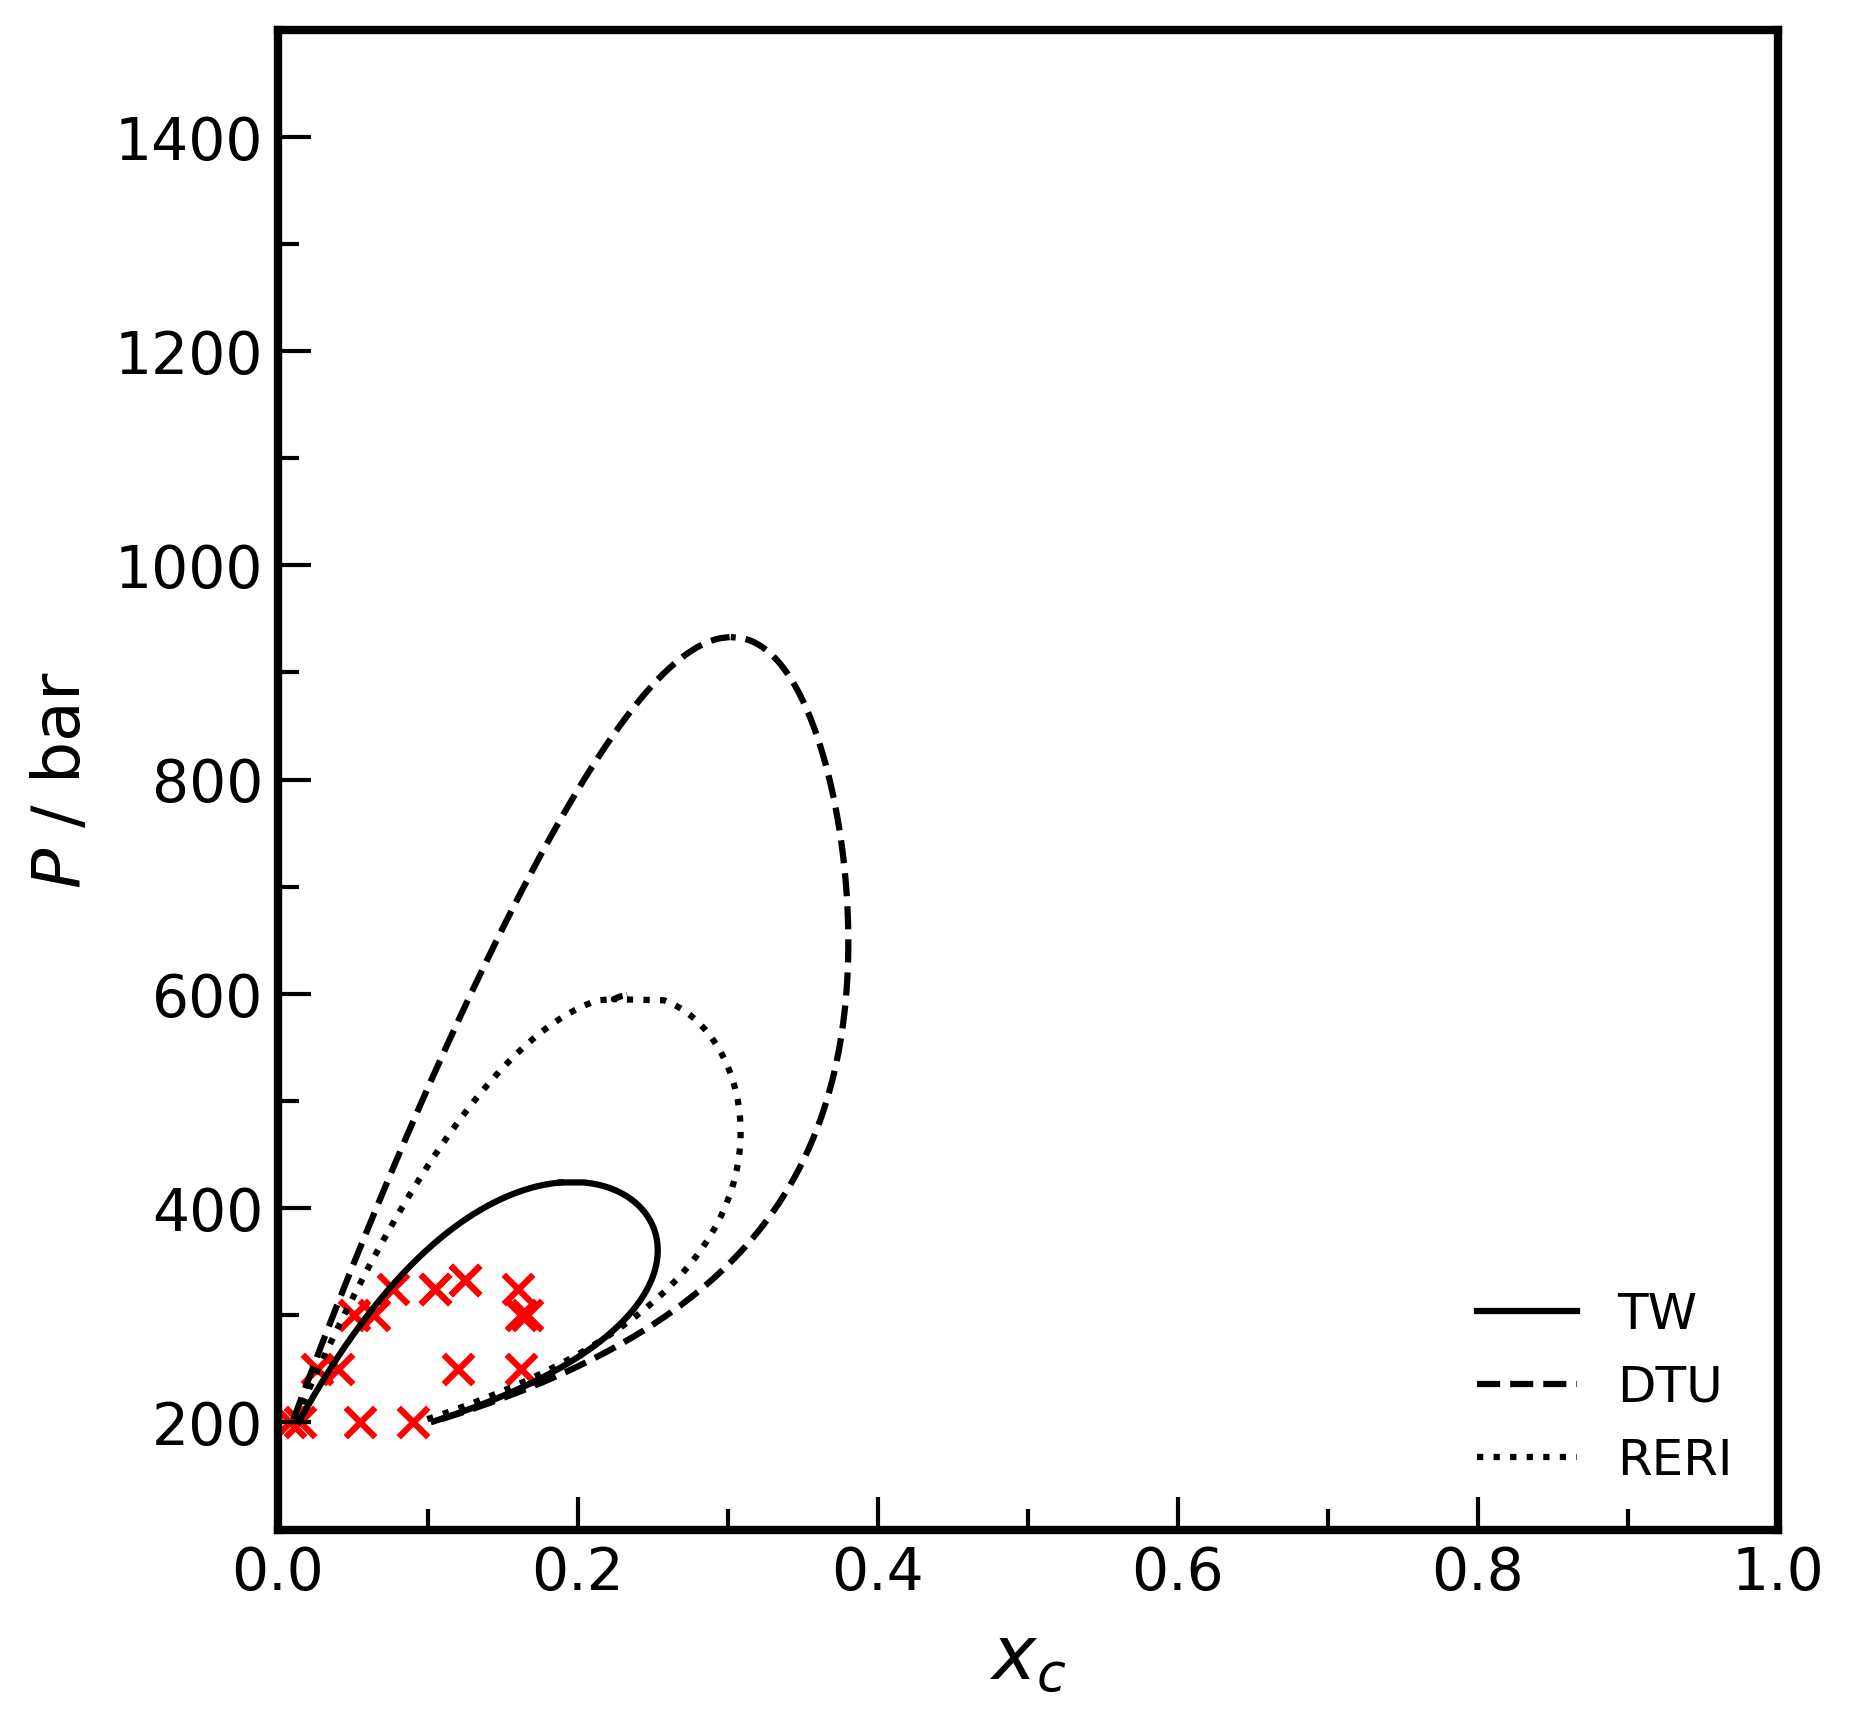
\includegraphics[width=.82\linewidth]{Figures/CPAmodels_T623K.png}
  \caption{$T$ = 623 K}
\end{subfigure}%
\label{TW_DTU_RERI2}
\caption{Phase diagram of the \ce{CO2}-\ce{H2O} mixture at various temperatures (a-d) from CPA EoS models (This Work (TW), DTU \cite{Tsivintzelis2011, Maribo2015, Olsen2021} and RERI \cite{Li2009}) and experiments \cite{Guo2014,  Tödheide1963, Takenouchi1964} (discrete points).} 
\end{figure}

\newpage

\begin{figure}[h!]
\begin{subfigure}{.33\textwidth}
  \centering
  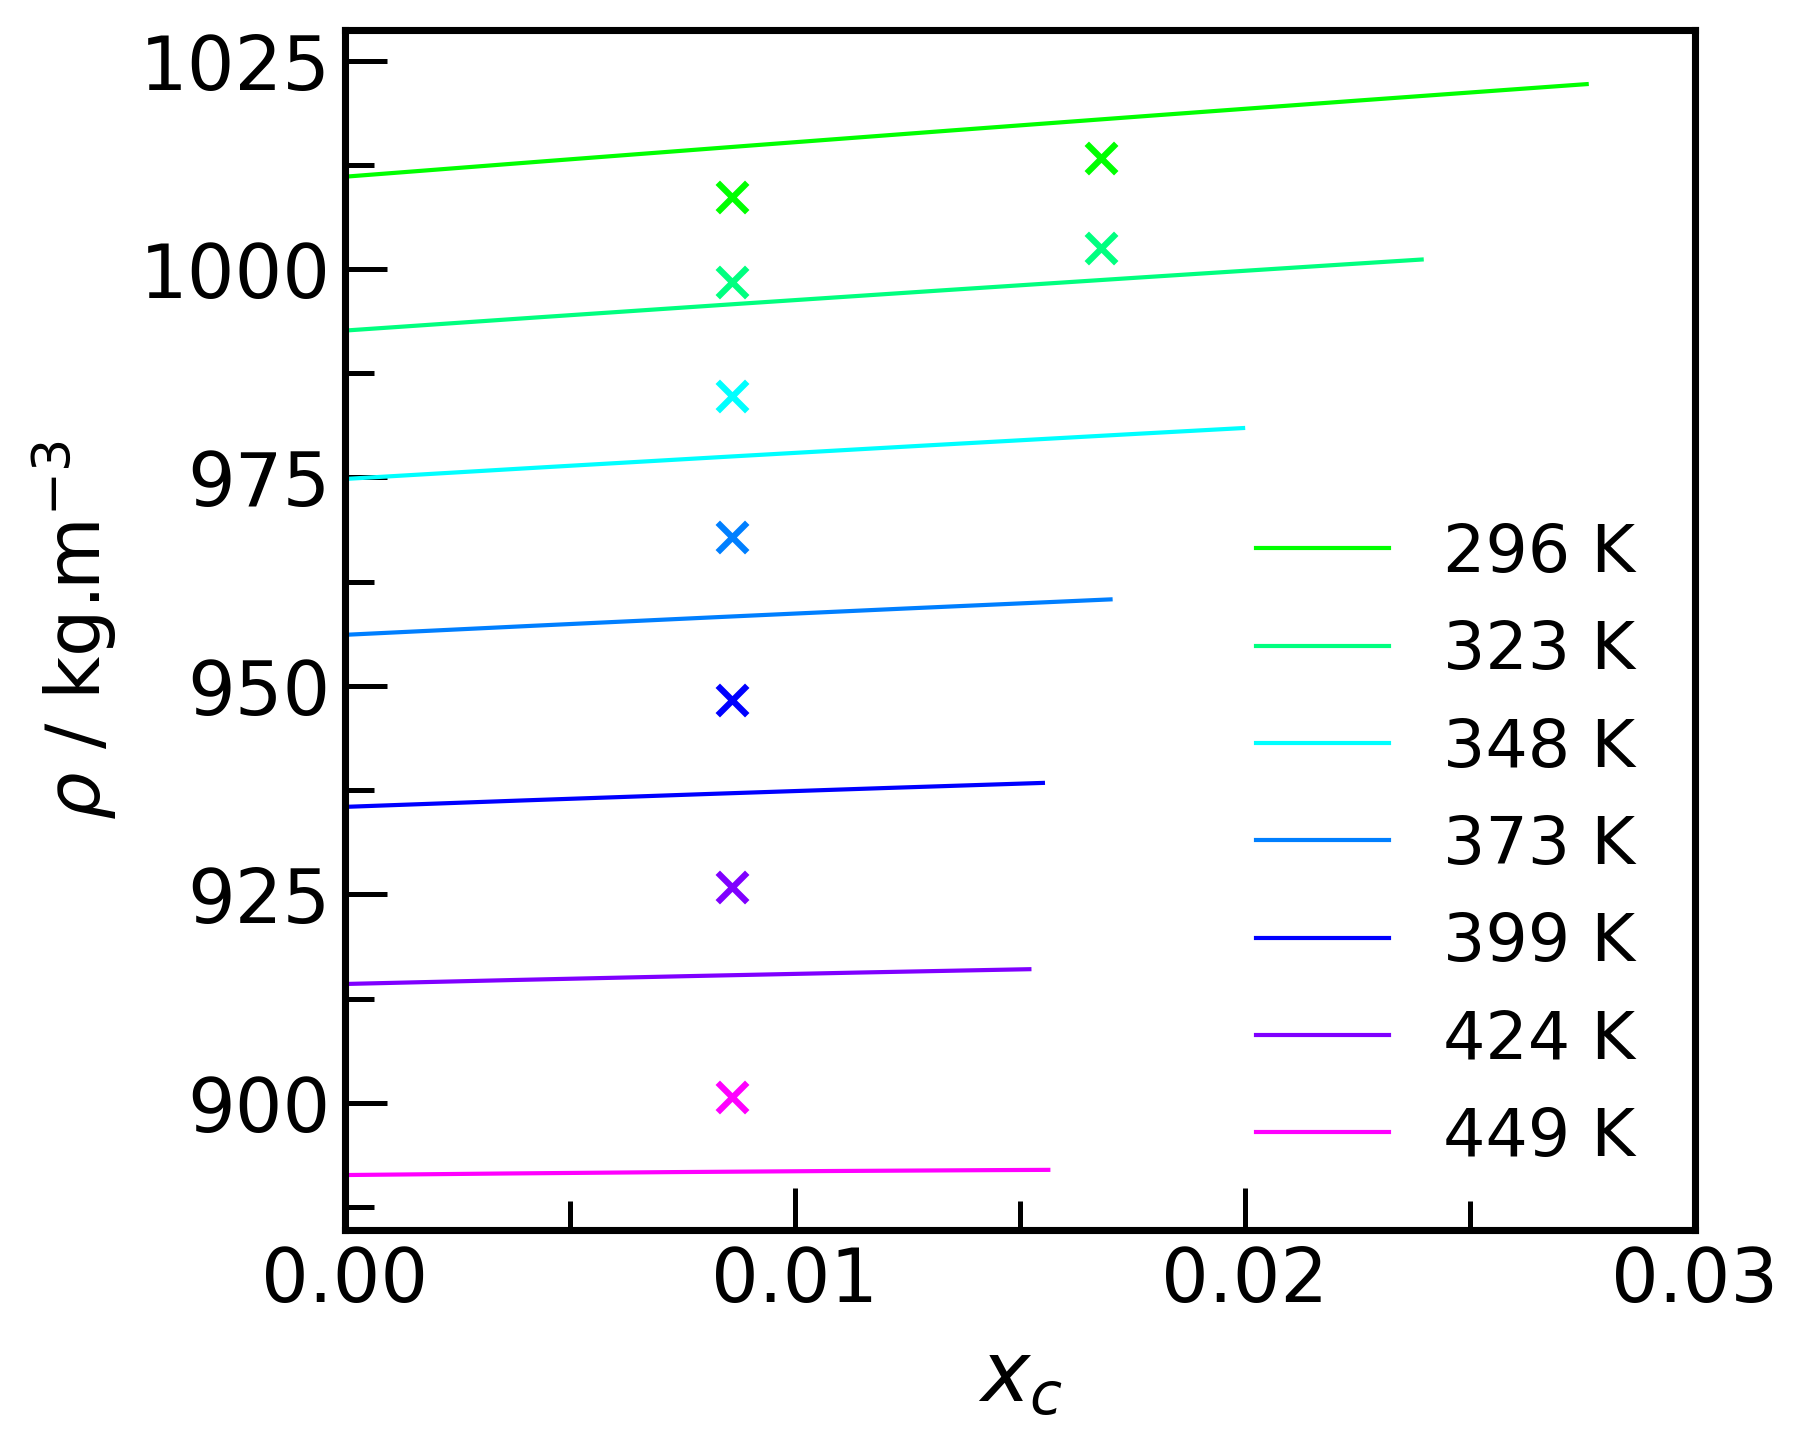
\includegraphics[width=.98\linewidth]{Figures/RHOCW_P150b.png}
  \caption{$P$ = 150 bar}
\end{subfigure}%
\begin{subfigure}{.33\textwidth}
  \centering
  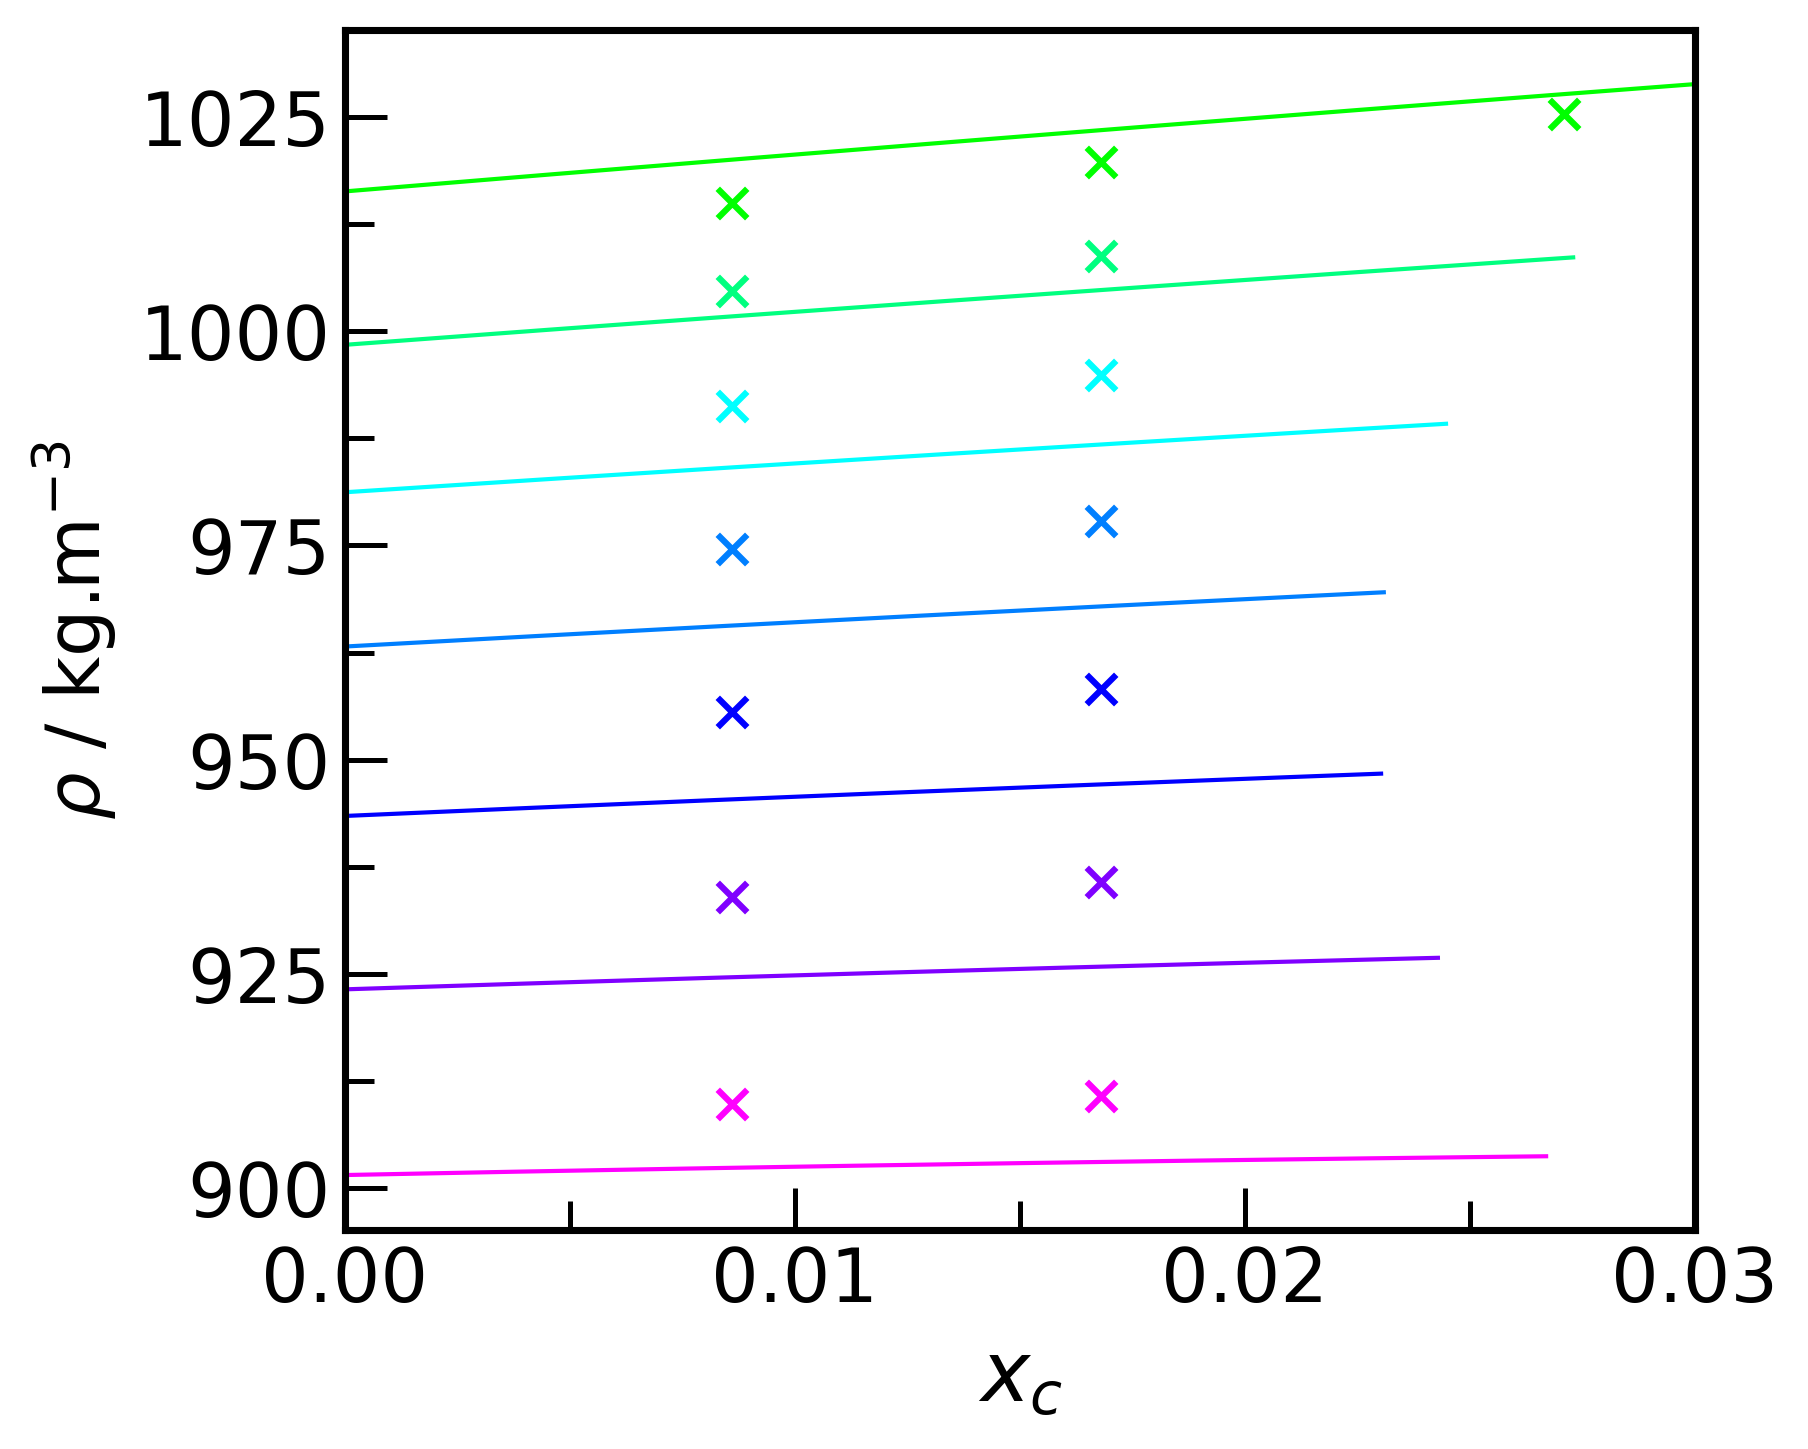
\includegraphics[width=.98\linewidth]{Figures/RHOCW_P302b.png}
  \caption{$P$ = 300 bar}
\end{subfigure}%
\begin{subfigure}{.33\textwidth}
  \centering
  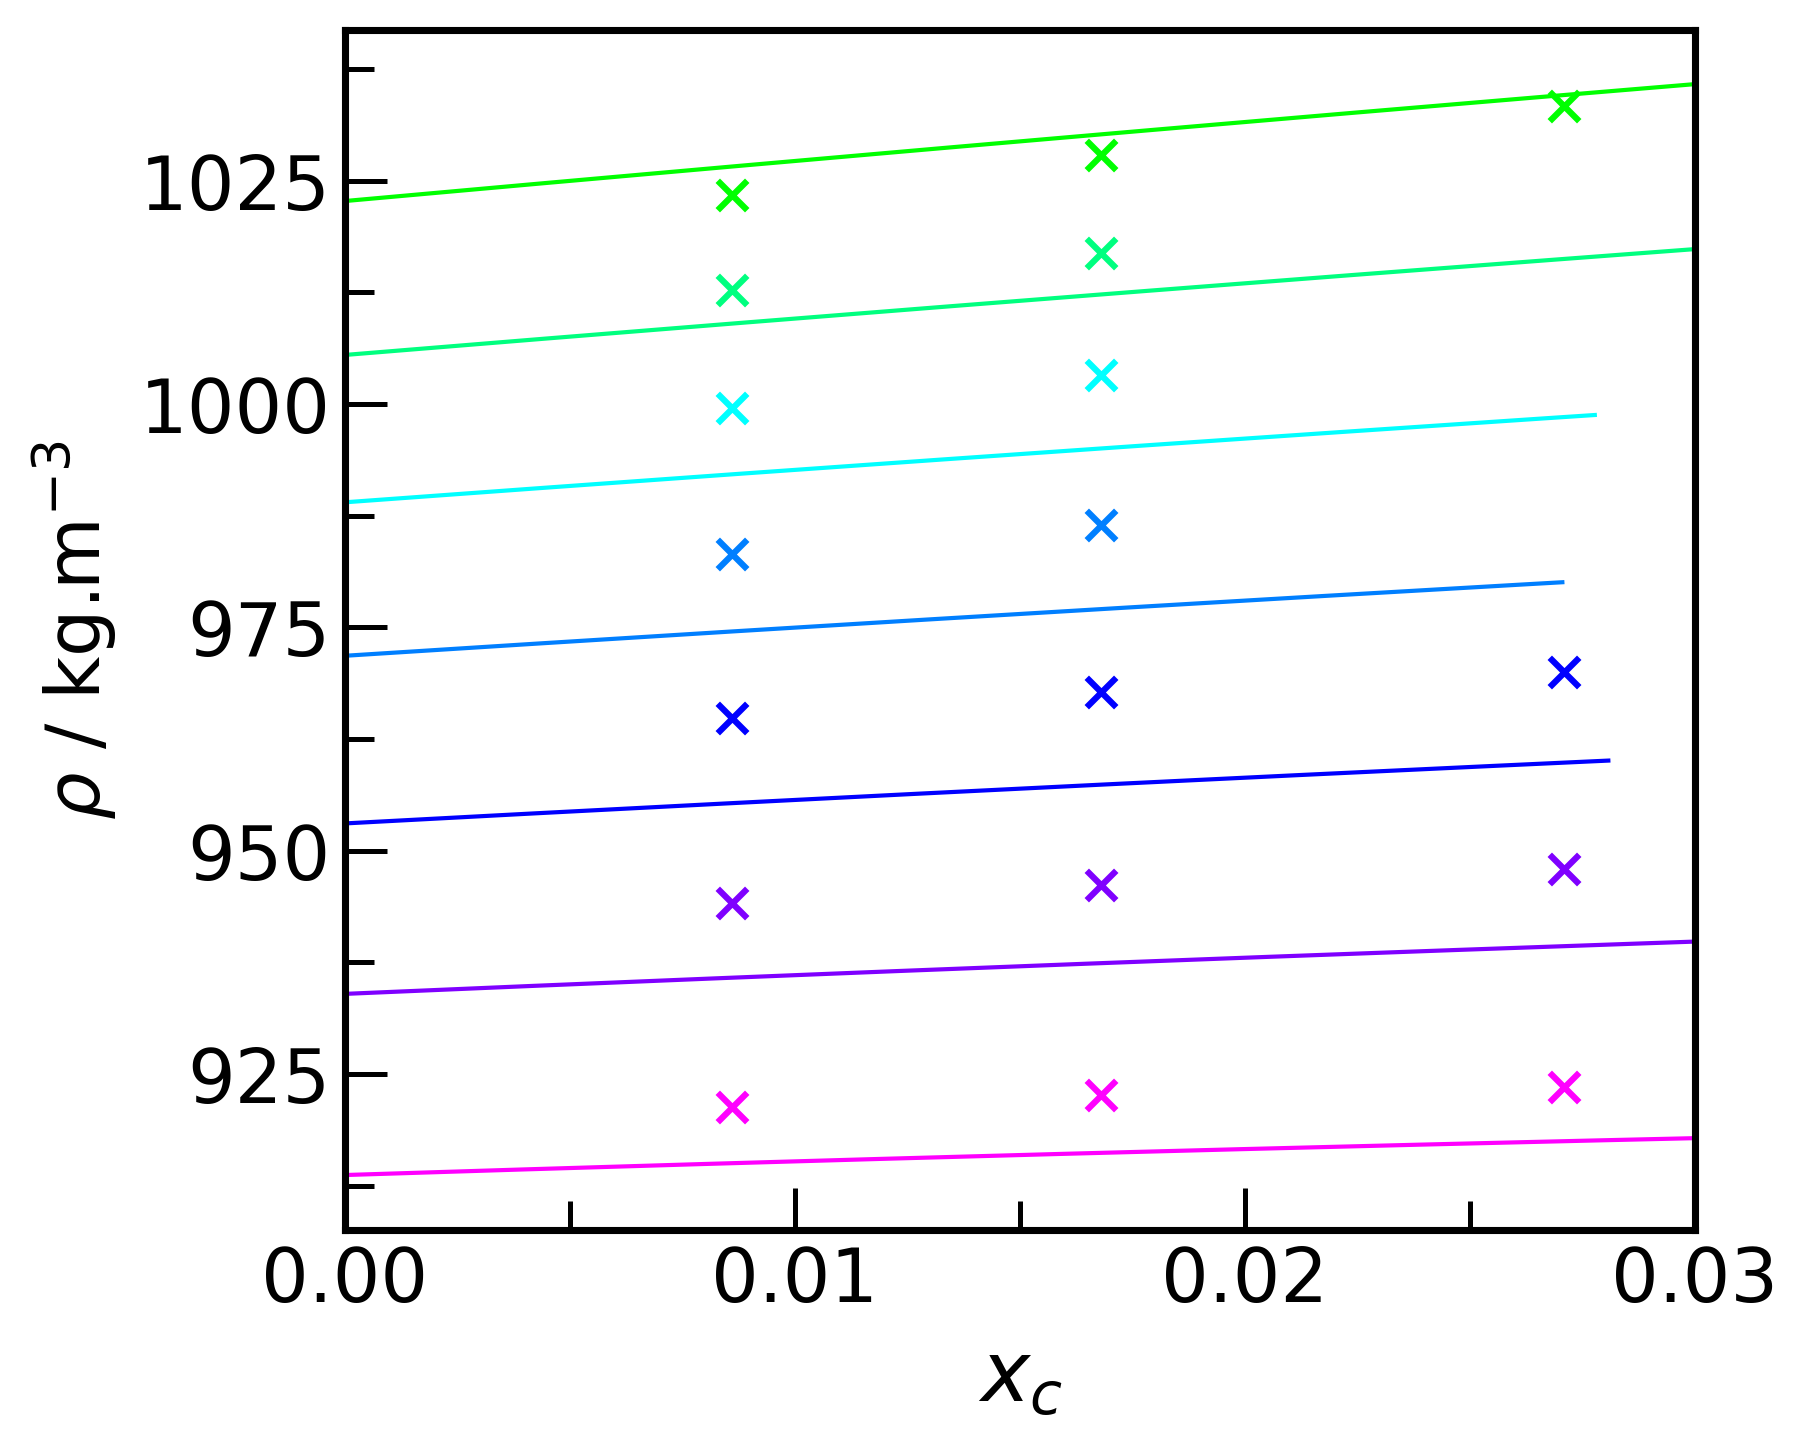
\includegraphics[width=.98\linewidth]{Figures/RHOCW_P503b.png}
  \caption{$P$ = 500 bar}
\end{subfigure}%
\vskip\baselineskip
\begin{subfigure}{.33\textwidth}
  \centering
  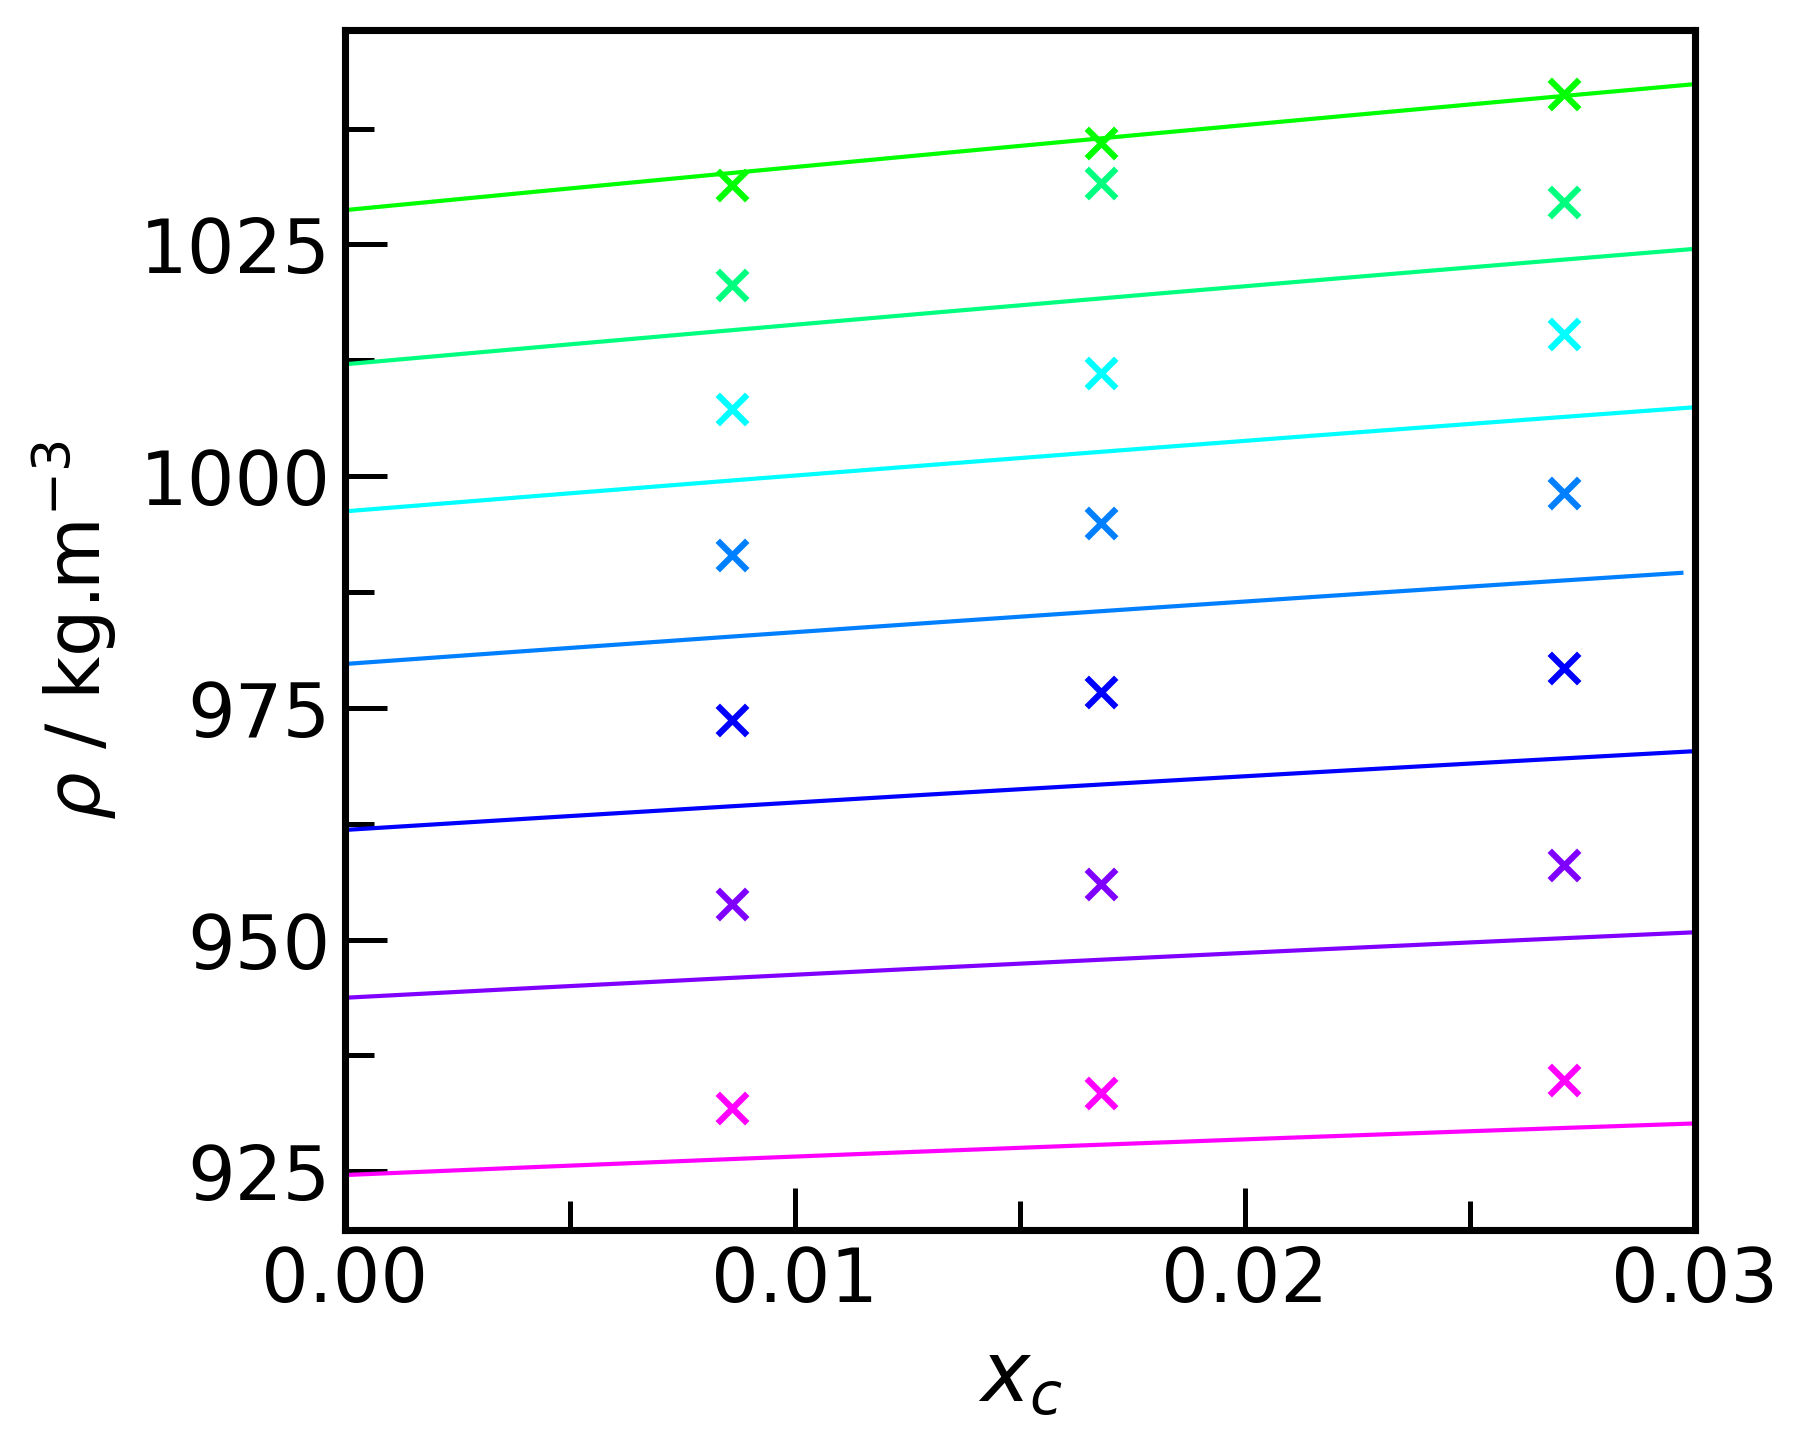
\includegraphics[width=.98\linewidth]{Figures/RHOCW_P705b.png}
  \caption{$P$ = 700 bar}
\end{subfigure}%
\begin{subfigure}{.33\textwidth}
  \centering
  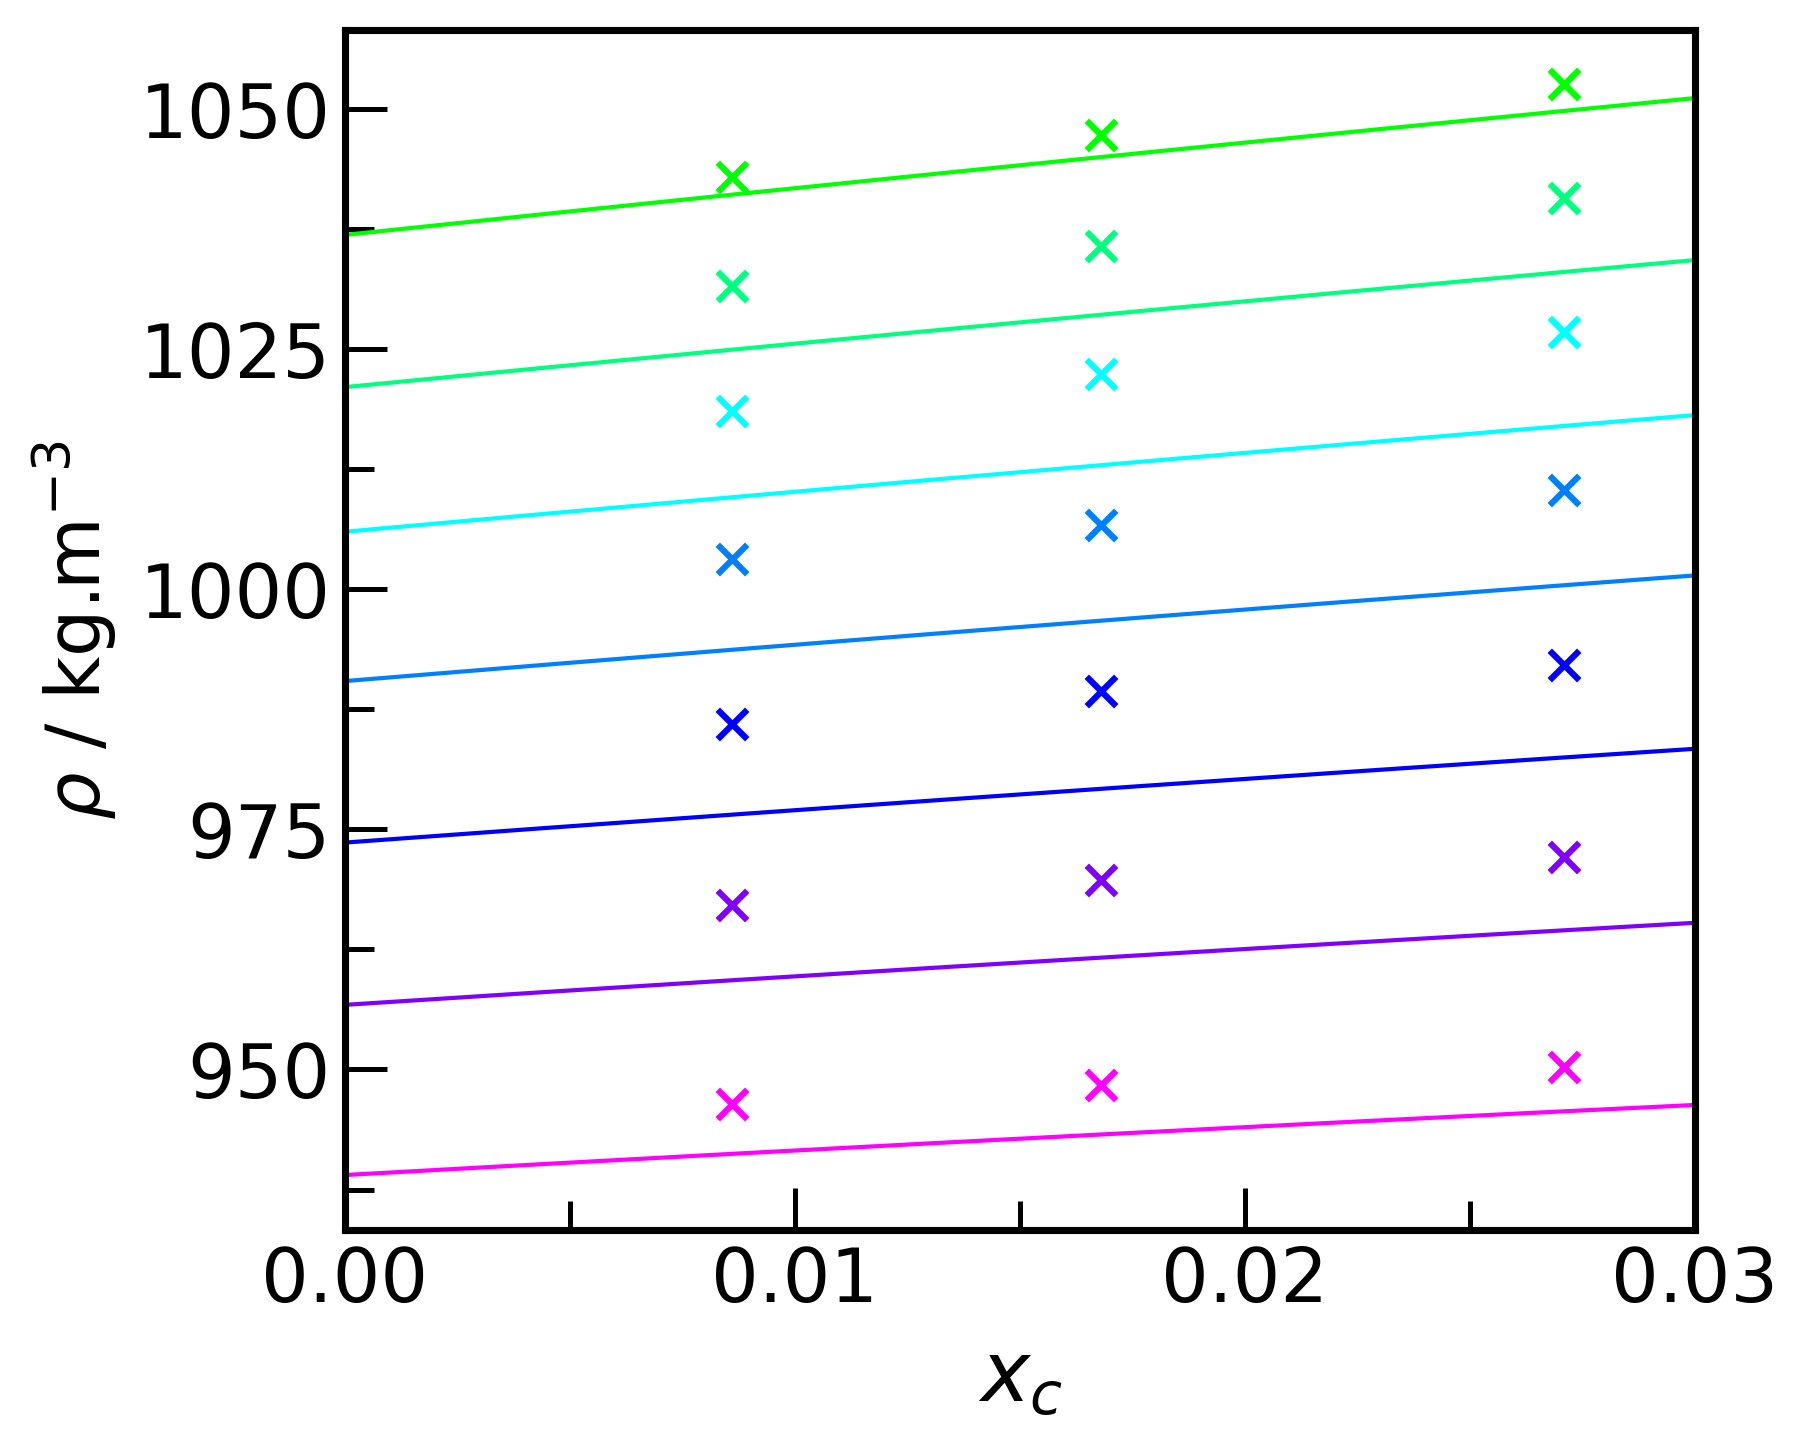
\includegraphics[width=.98\linewidth]{Figures/RHOCW_P1007b.png}
  \caption{$P$ = 1000 bar}
\end{subfigure}%
\label{RHO_CW}
\caption{Density of \ce{CO2}-water mixture in the aqueous phase below the saturation point \textit{vs.} \ce{CO2} concentration at various temperatures (the legend in the subplot (a) holds for all others) and various pressures (a-e) from CPA EoS (continuous line) and experiments \cite{Wright2015} (discrete points).}
\end{figure}

\newpage

\begin{figure}[h!]
\centering
  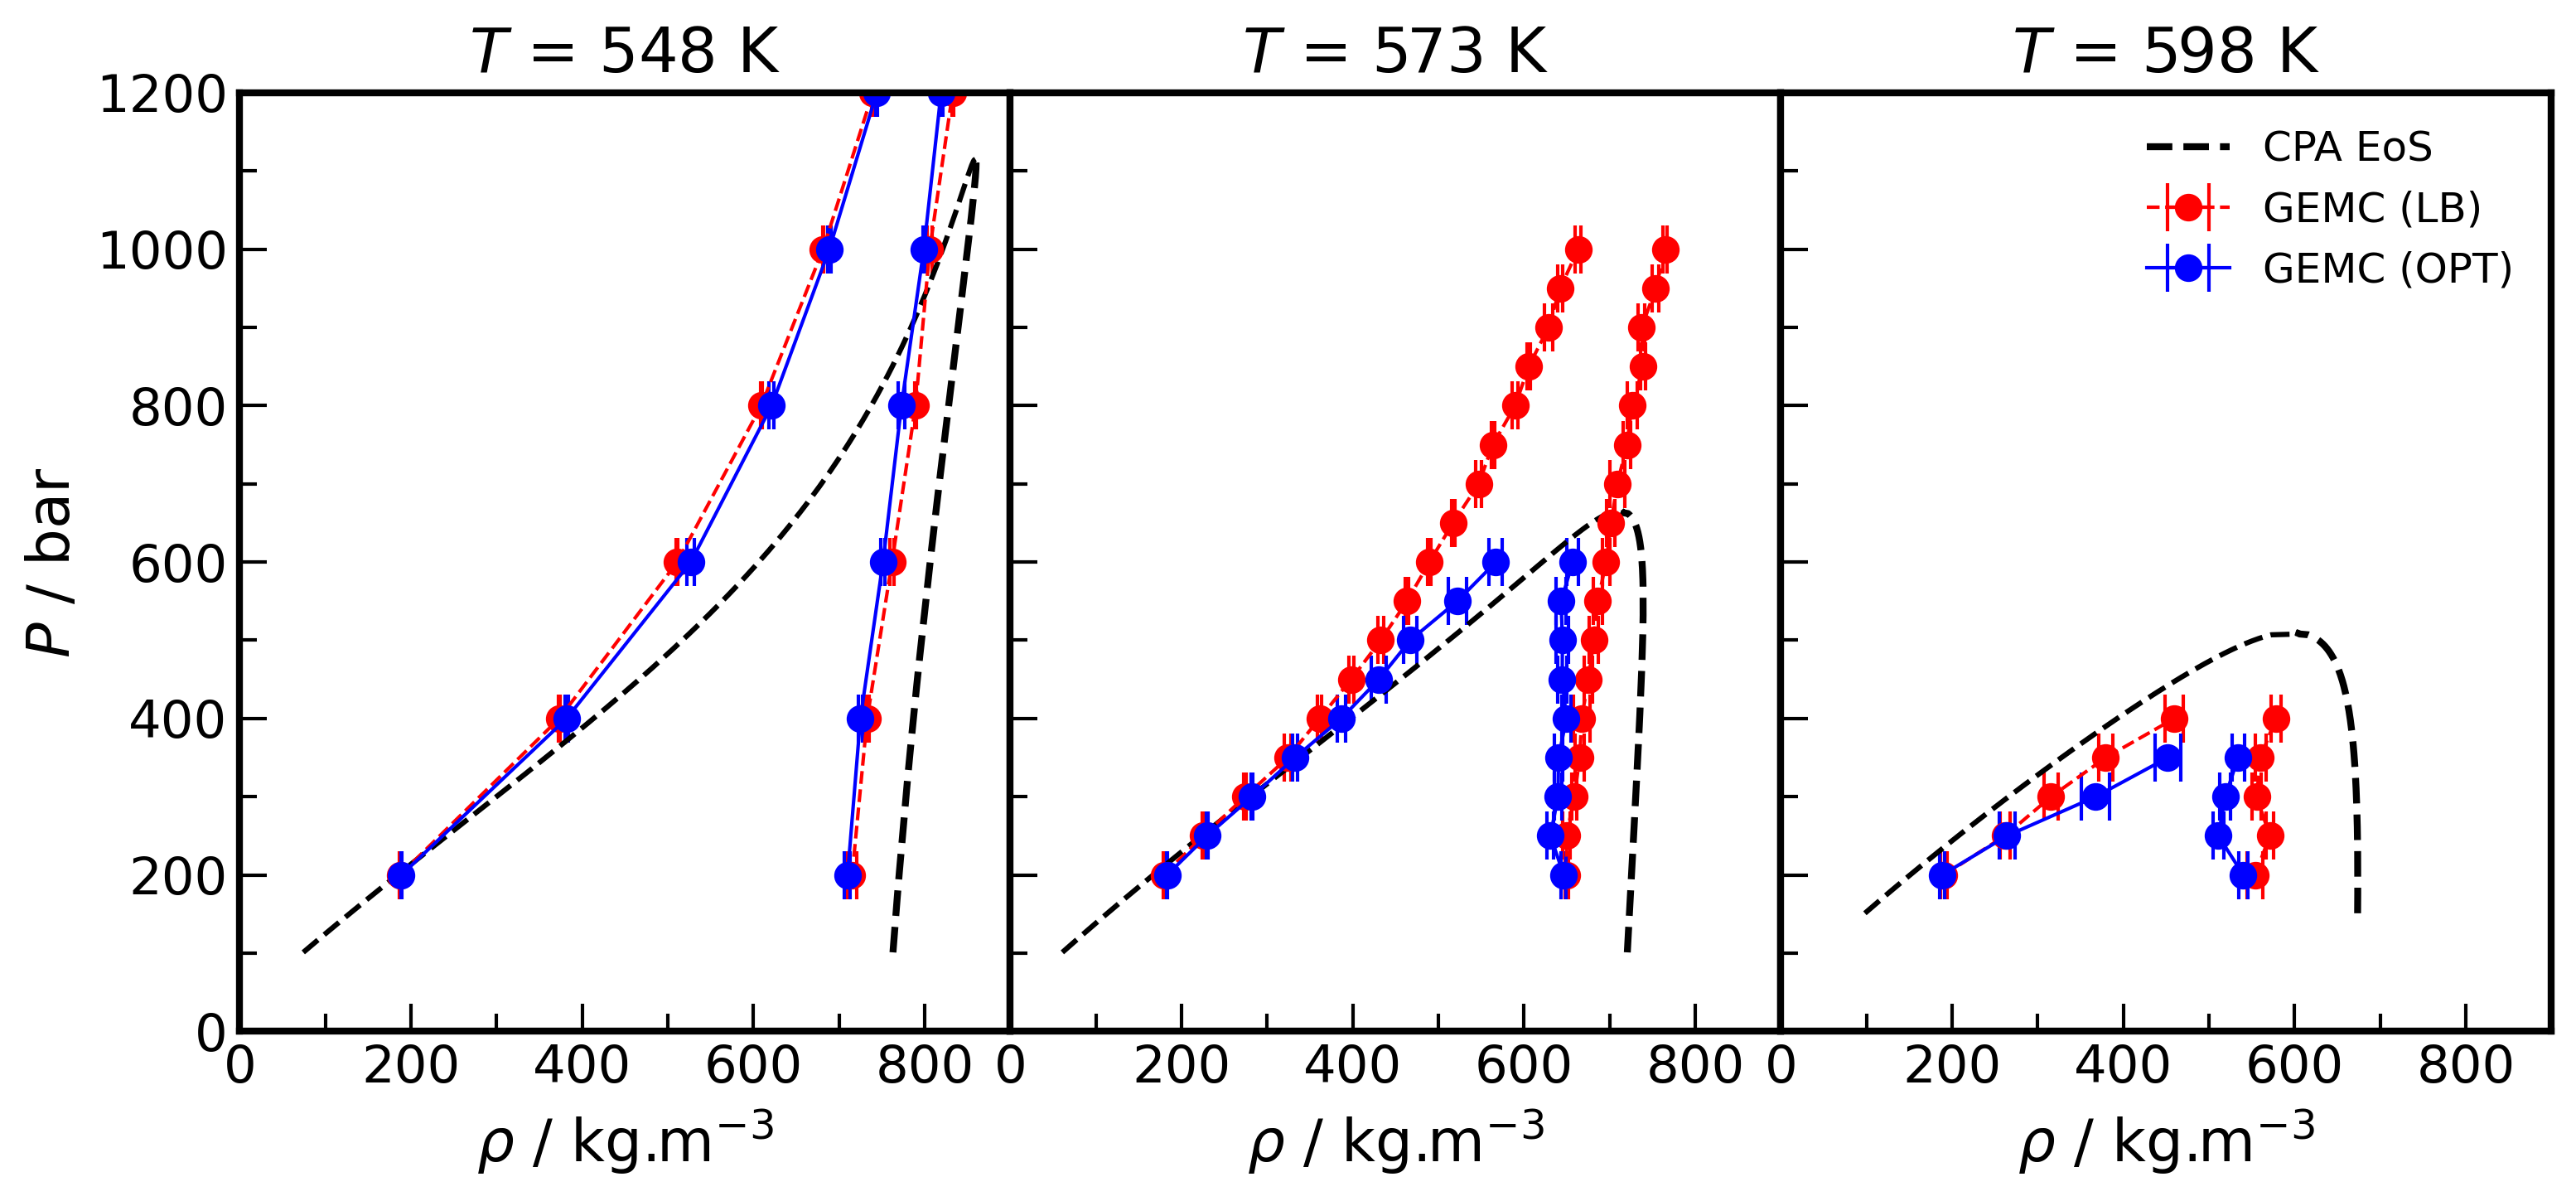
\includegraphics[width=0.95\textwidth]{Figures/GEMCvsCPA_CW_rho.png} 
\label{GEMC_RHO_CW}
\caption{Density of the aqueous and \ce{CO2}-rich phases at equilibrium in the \ce{CO2}-\ce{H2O} mixture at various temperatures from GEMC simulations and CPA EoS. "LB" and "OPT" stand for Lorentz-Berthelot and optimized (at lower temperatures \cite{Vlcek2011}) unlike parameters between \ce{CO2}-\ce{H2O} molecules, respectively.}
\end{figure}

\newpage


\begin{figure}[h!]
\centering
  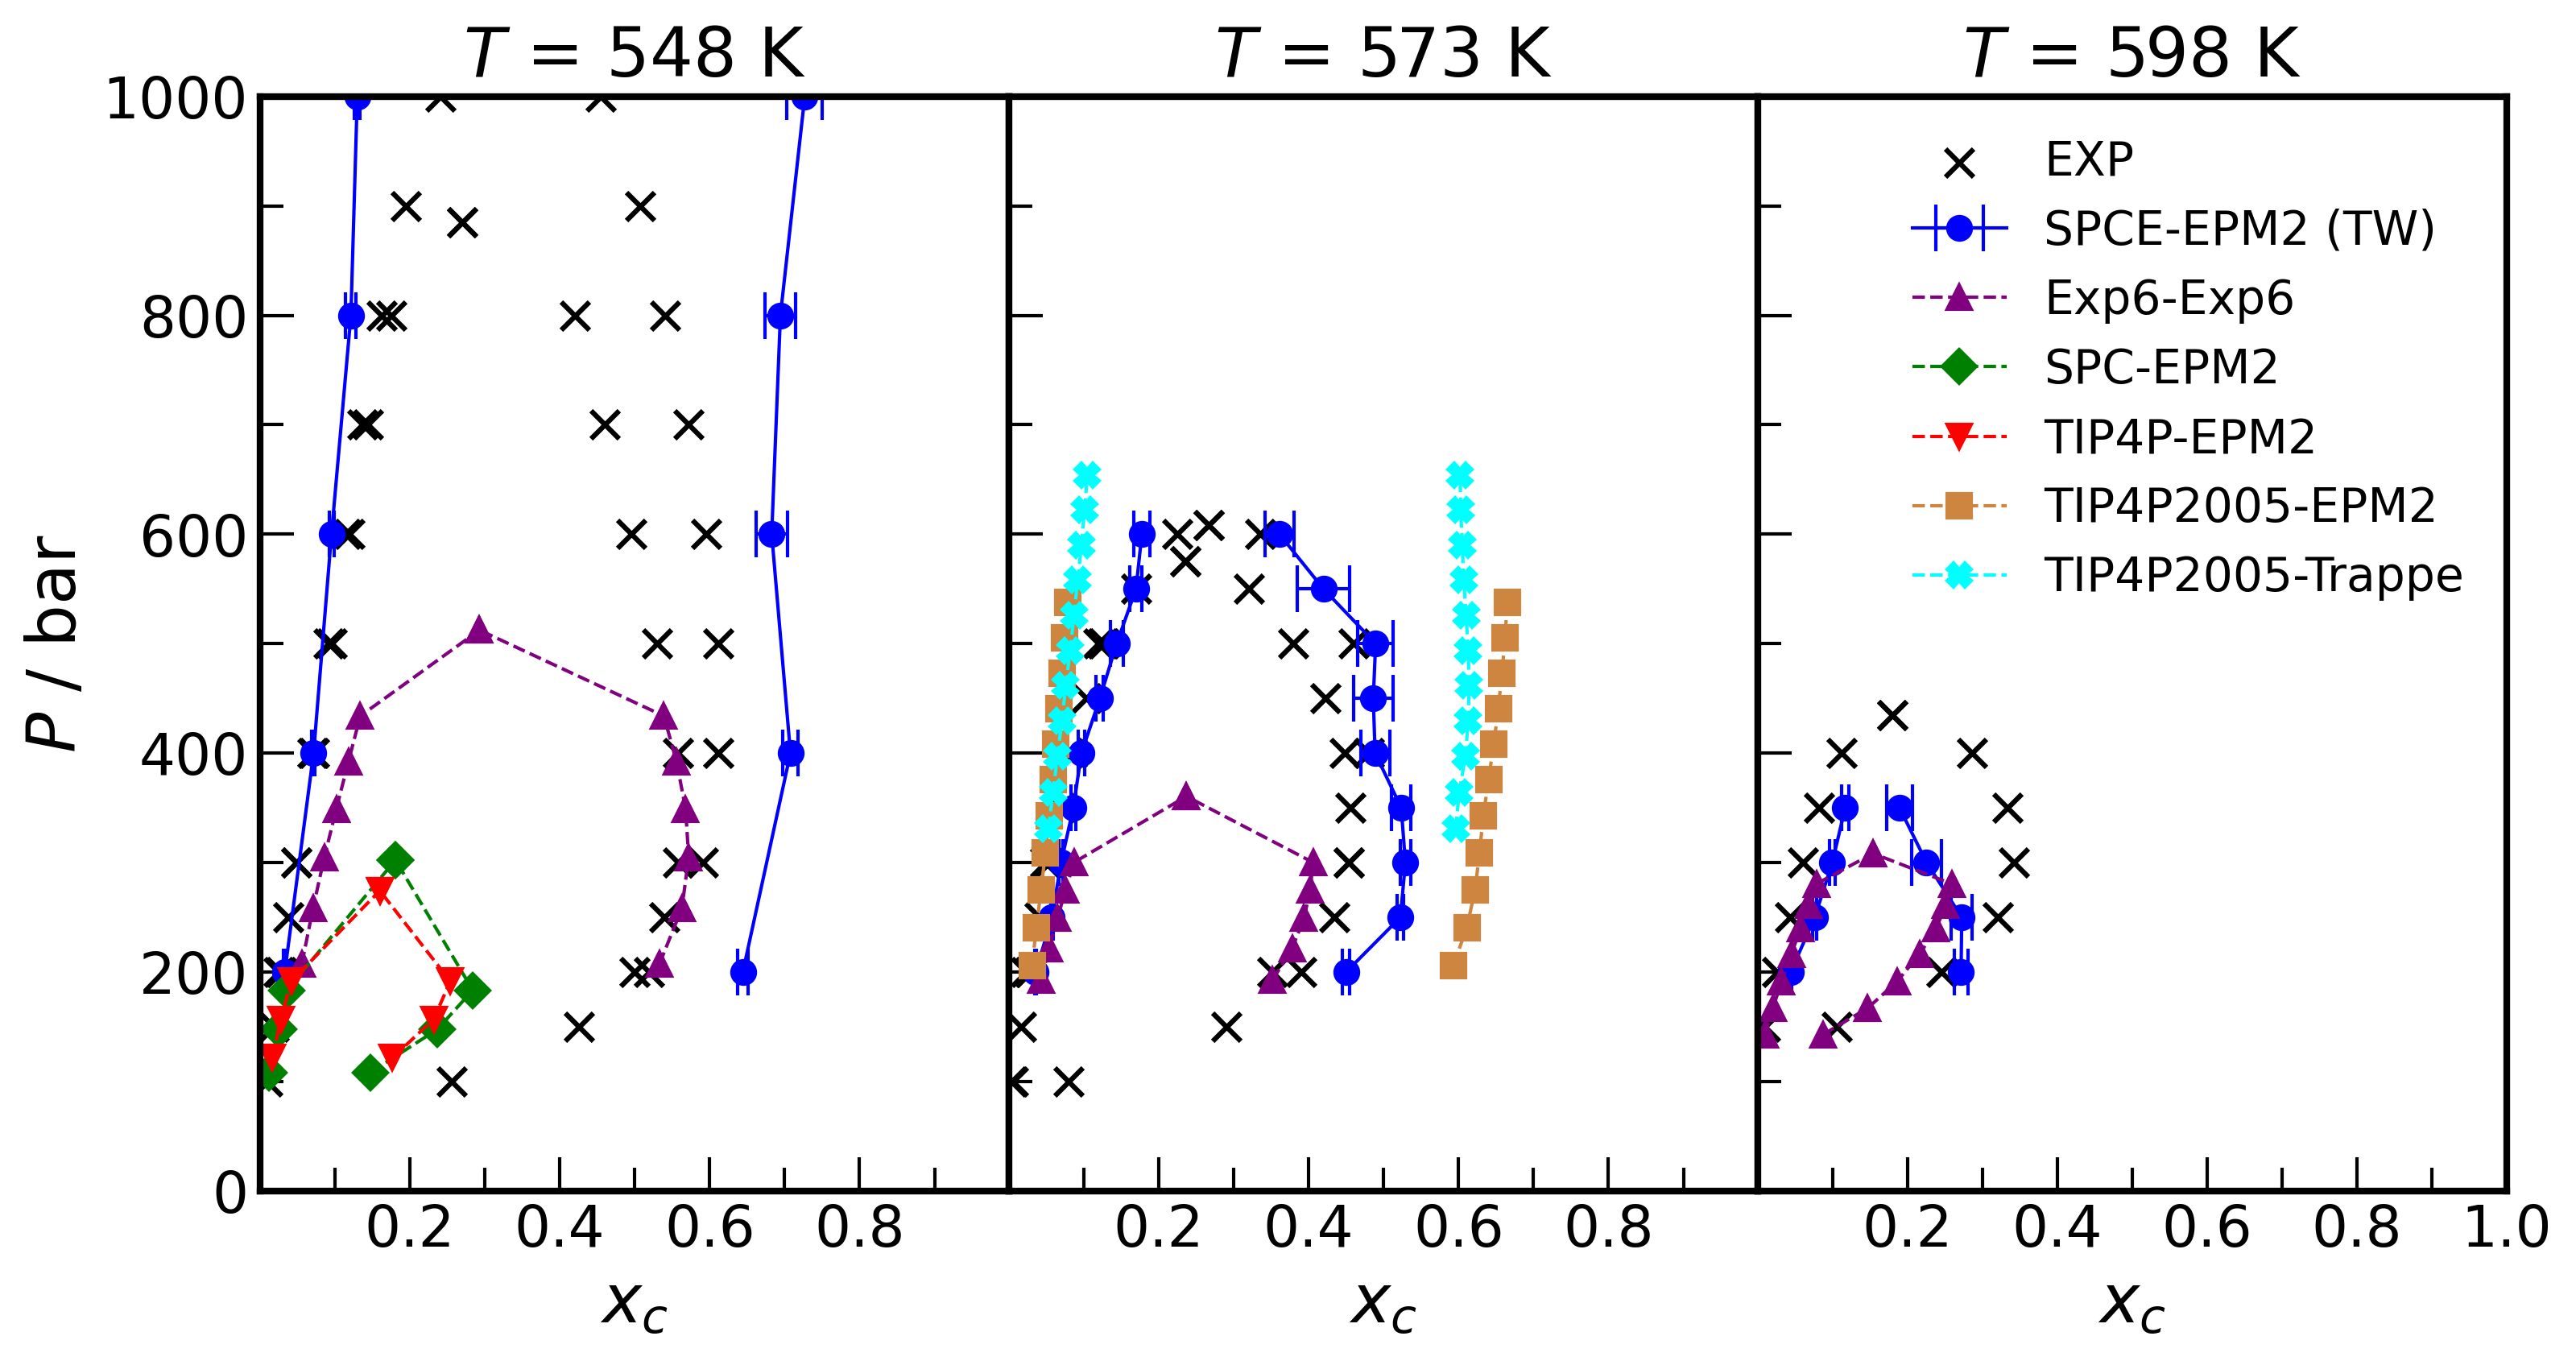
\includegraphics[width=0.8\textwidth]{Figures/GEMC_FFs.png} 
\caption{Phase diagram of the \ce{CO2}-\ce{H2O} mixture at various temperatures from GEMC simulations and experiments \cite{Guo2014, Tödheide1963, Takenouchi1964} for various classical force field combinations: SPCE-EPM2 (results from This Work using "OPT" unlike parameters), Exp6-Exp6 \cite{Liu2011}, SPC-EPM2 \cite{Liu2011}, TIP4P-EPM2 \cite{Liu2011}, TIP4P2005-EPM2 \cite{Liu2011}, TIP4P2005-Trappe \cite{Liu2011}.}
\label{GEMC_FFs1}
\end{figure}

\begin{figure}[h!]
\centering
  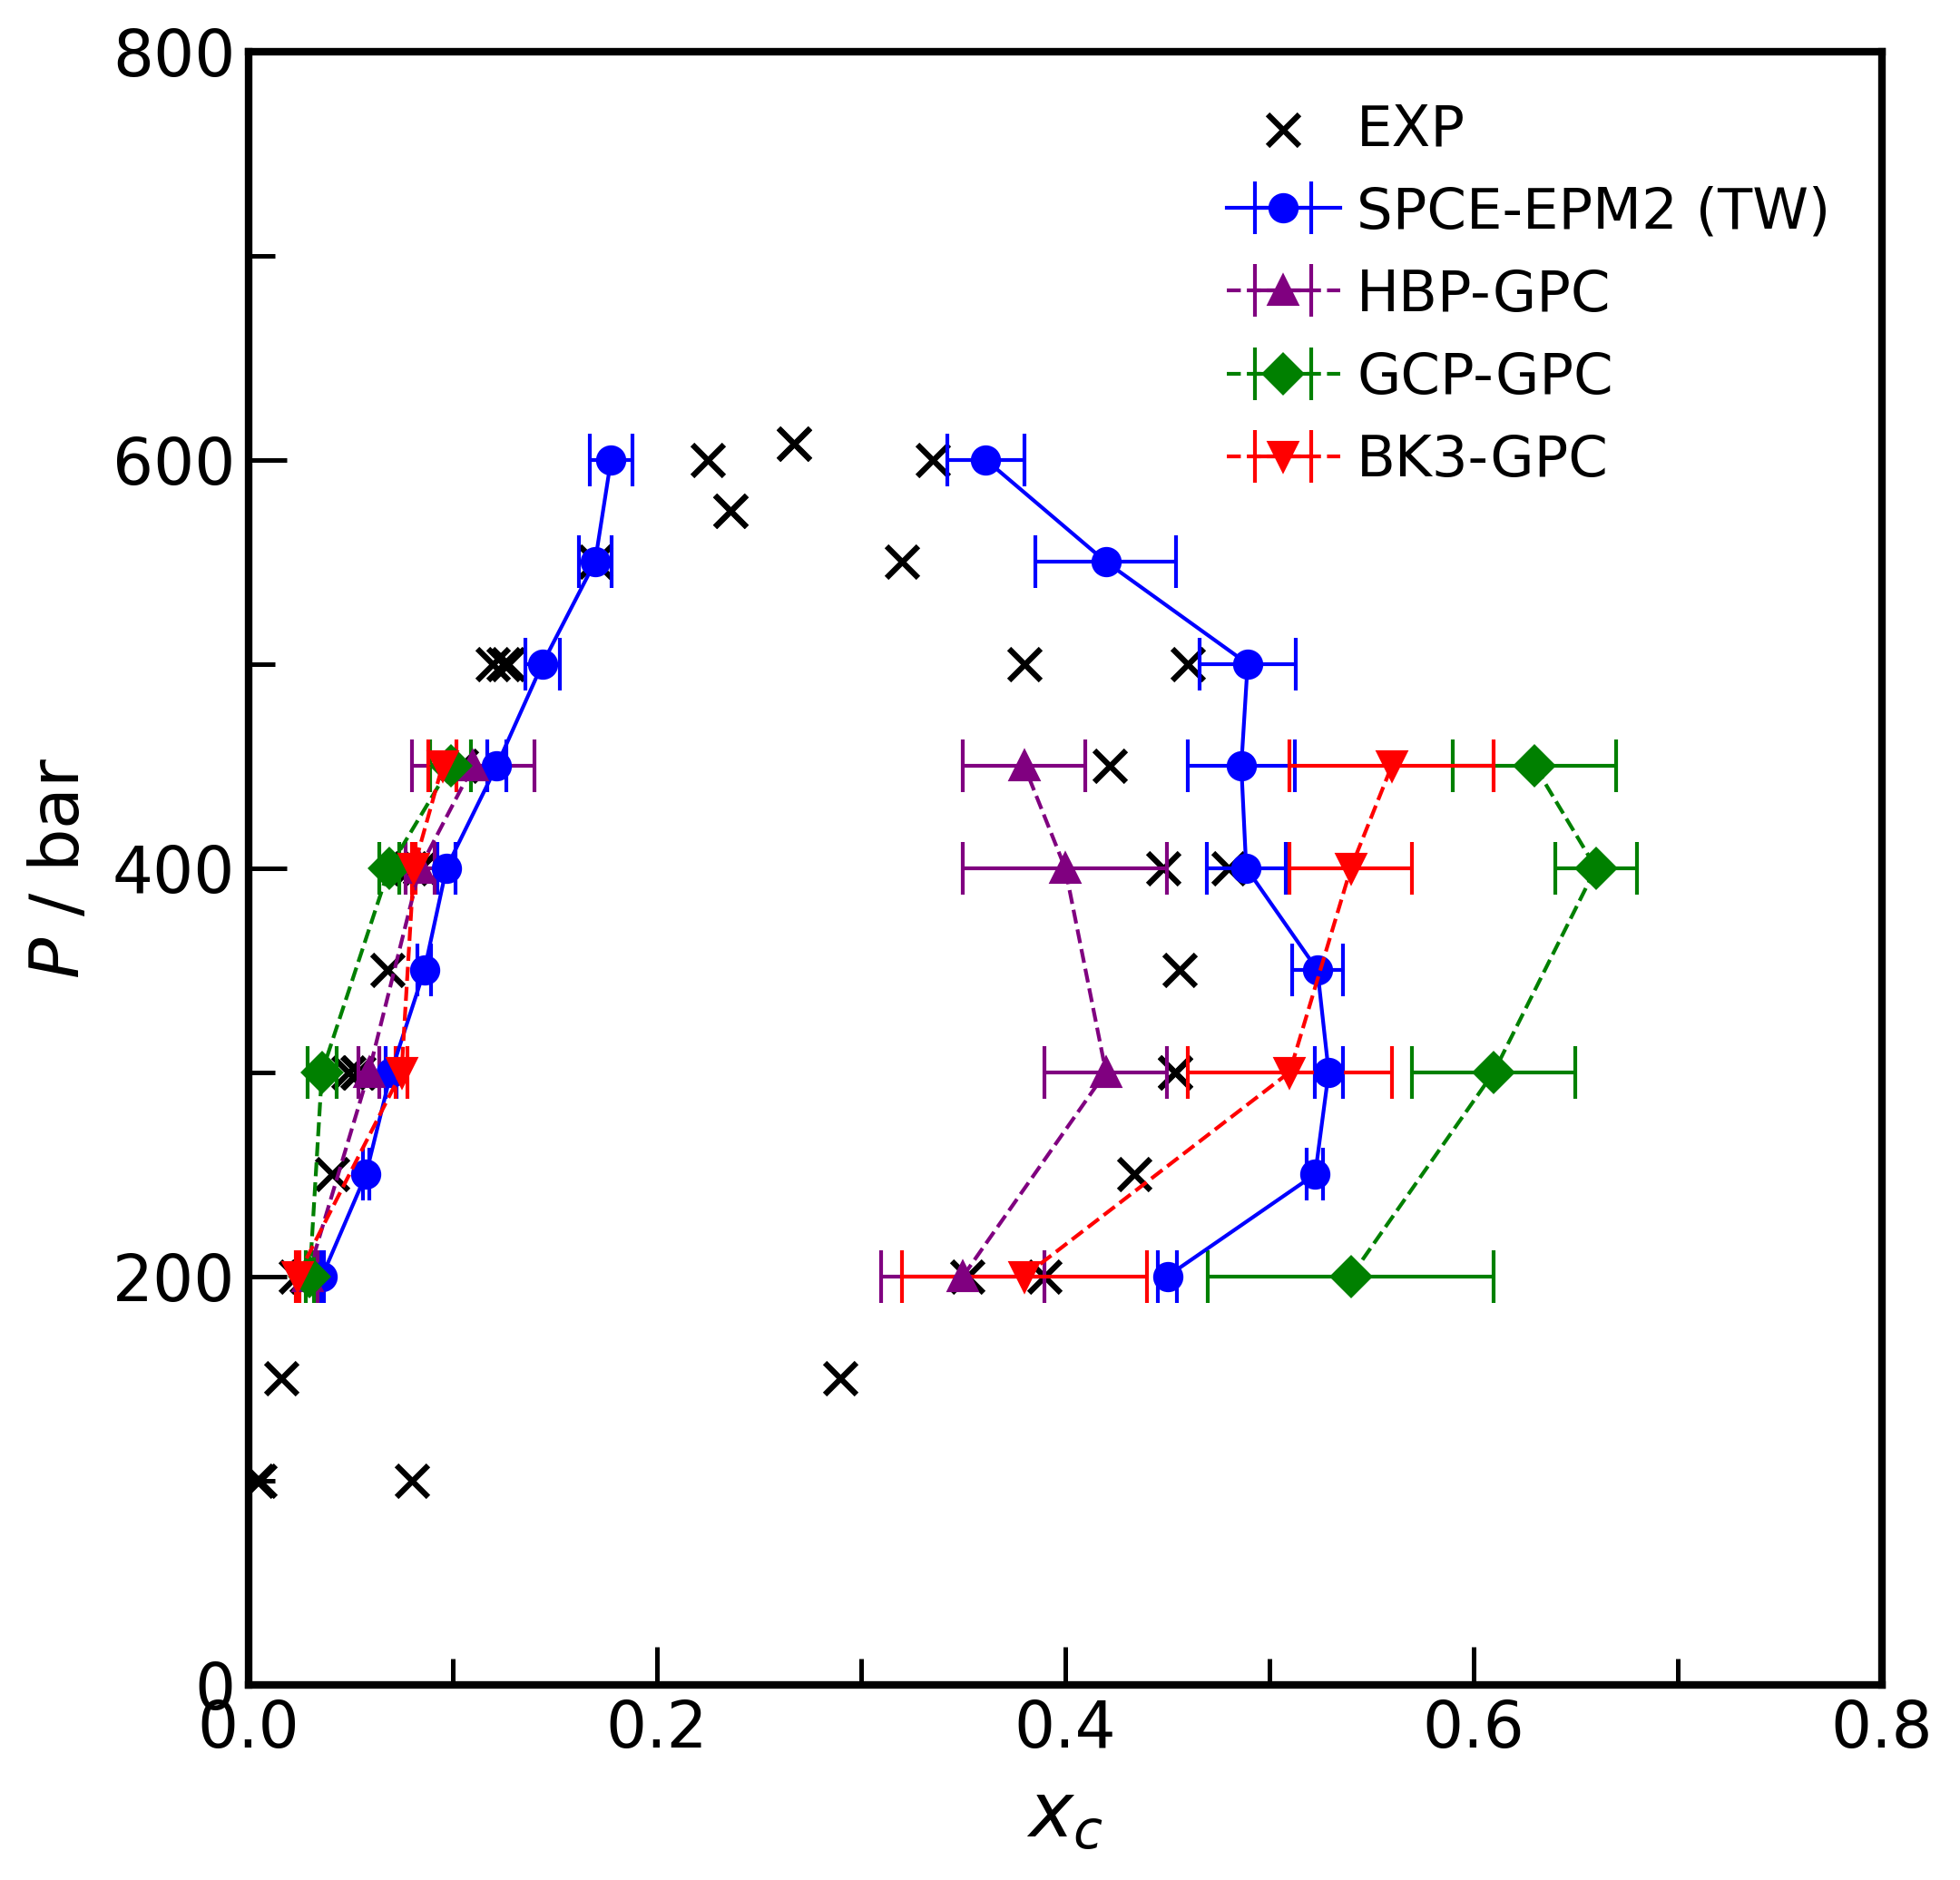
\includegraphics[width=0.5\textwidth]{Figures/GEMC_FFpol_T573K.png} 
\label{GEMC_FFs2}
\caption{Phase diagram of the \ce{CO2}-\ce{H2O} mixture at $T$ = 573 K from GEMC simulations and experiments \cite{Guo2014, Tödheide1963, Takenouchi1964} for various polarizable force field combinations: HBP-GPC \cite{Jiang2017a}, GCP-GPC \cite{Jiang2017a} and BK3-GPC \cite{Jiang2017a}. We also show the results from the classical force field SPCE-EPM2 (results from This Work using "OPT" unlike parameters).}
\end{figure}



\newpage

\section{\ce{CO2}-Brine Mixture}

\begin{figure}[h!]
\centering
  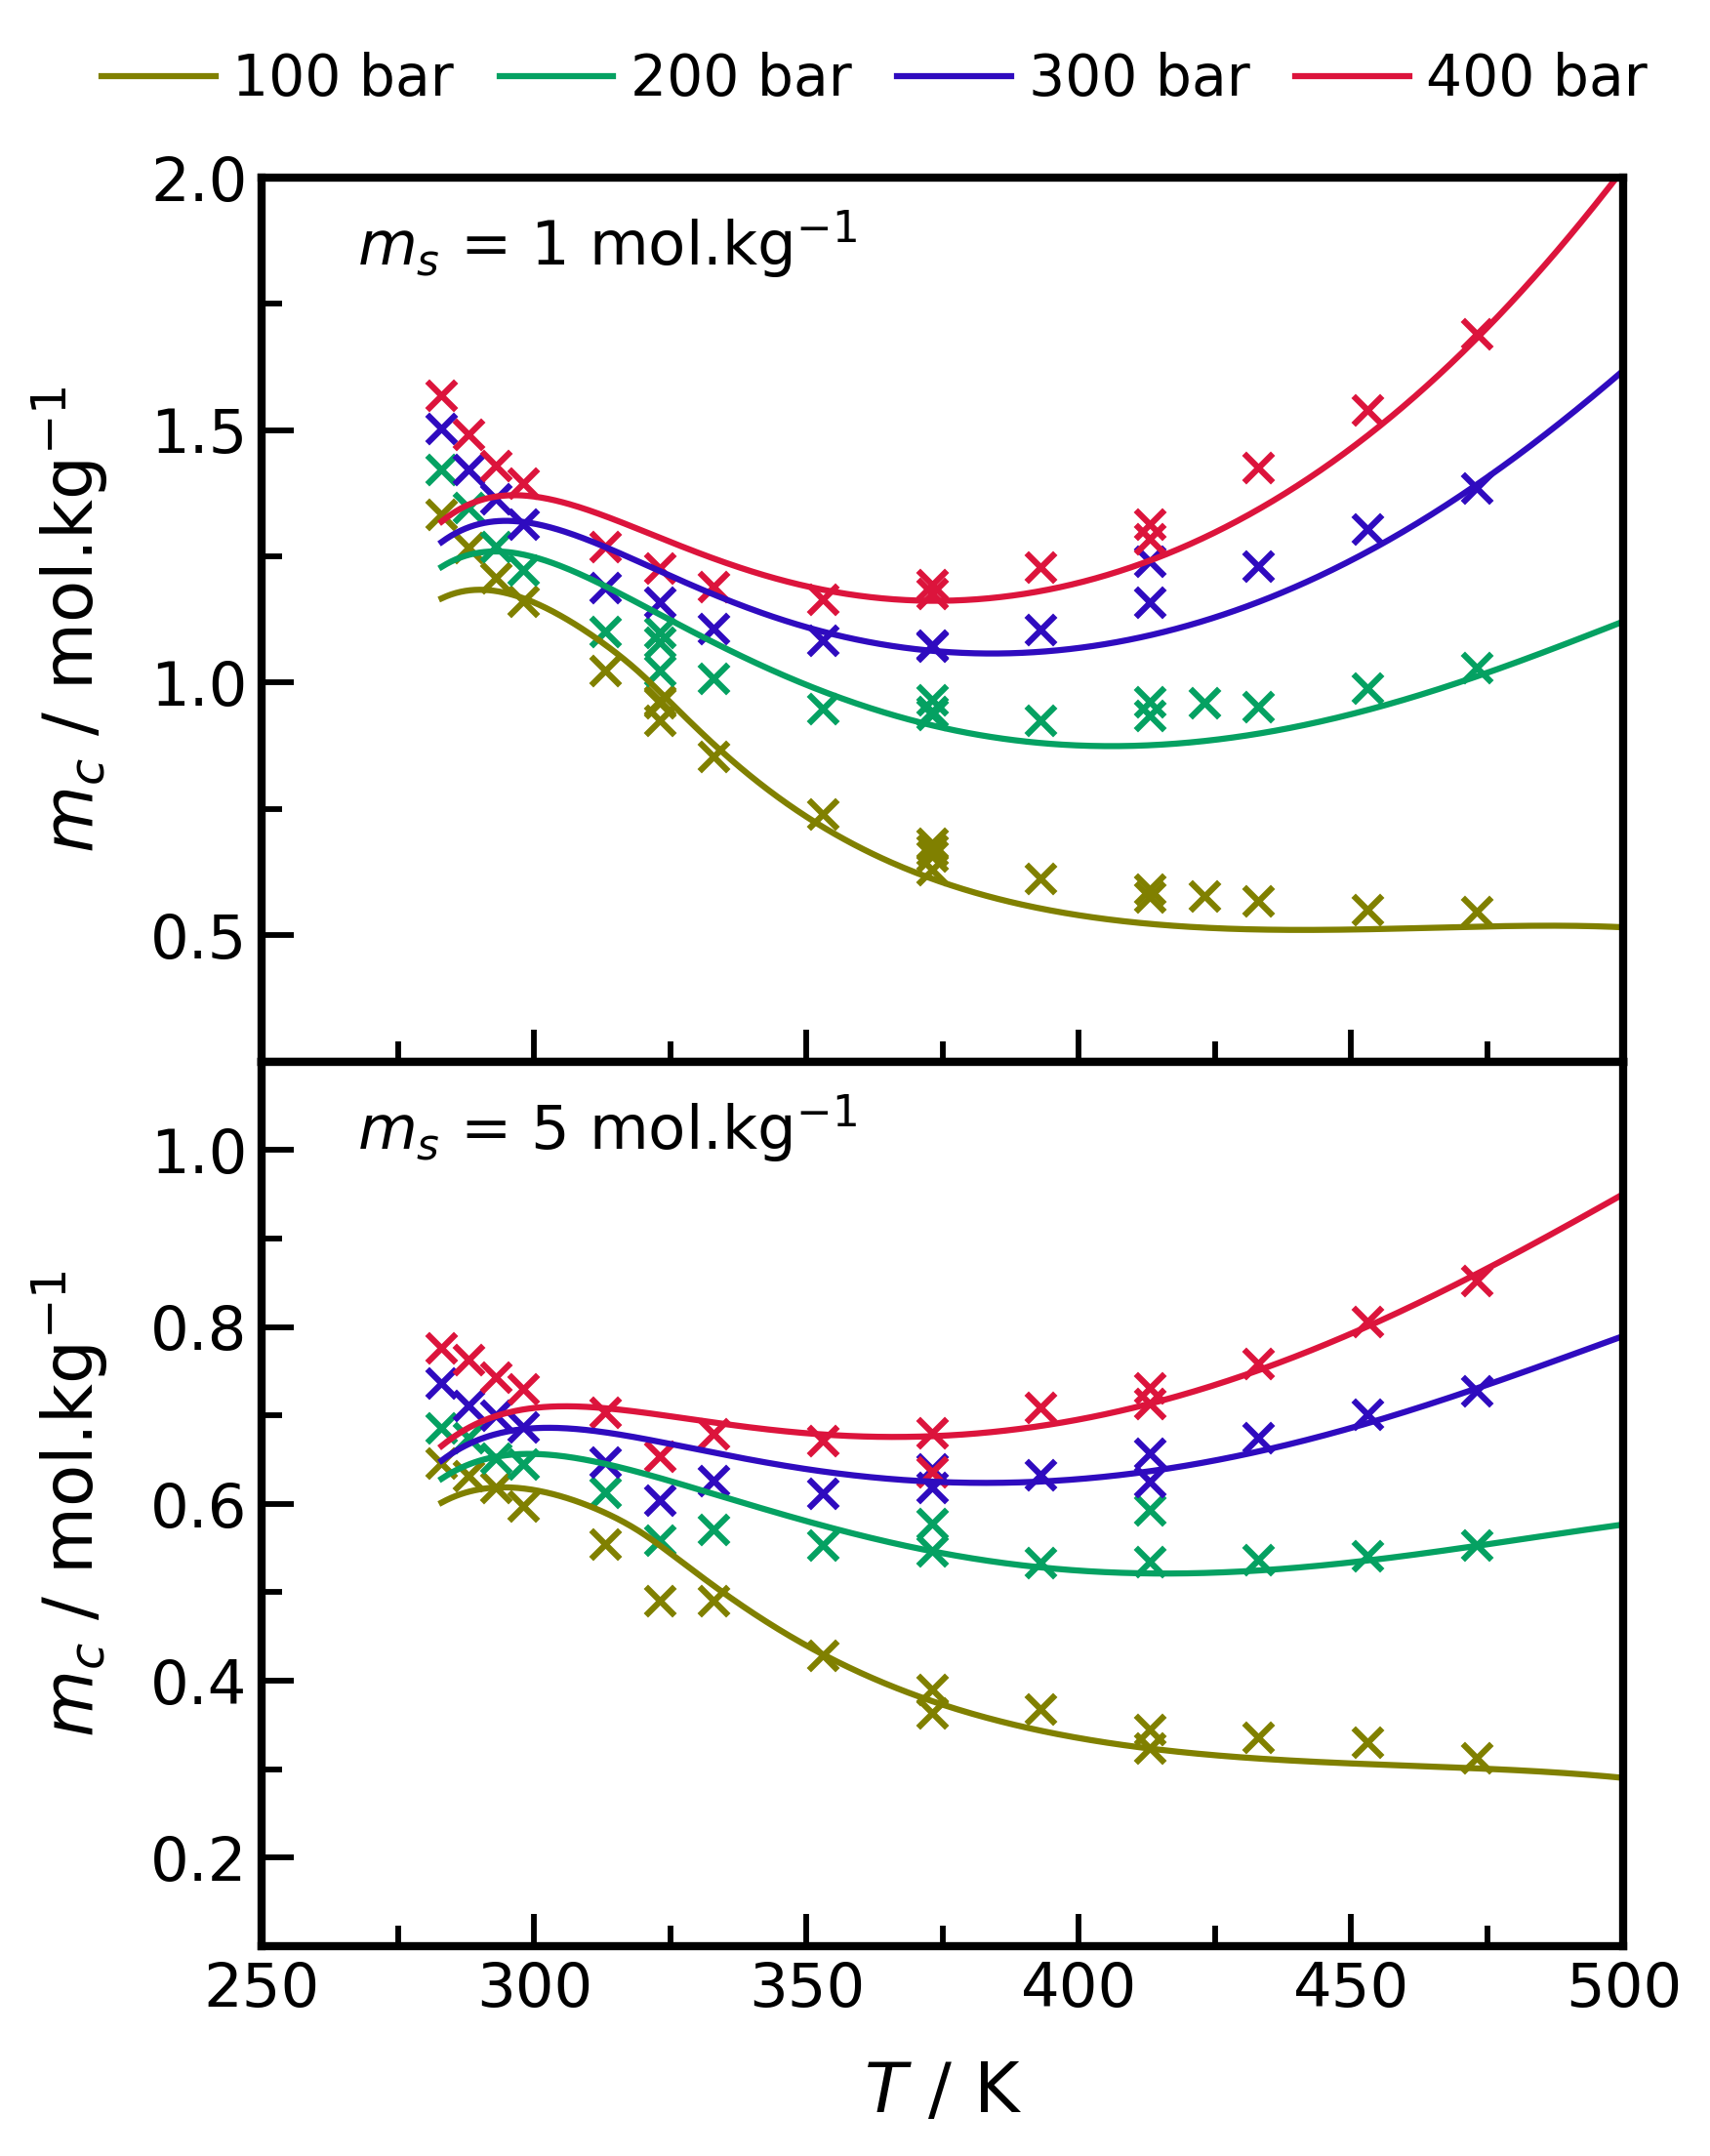
\includegraphics[width=0.65\textwidth]{Figures/eCPA_Tlow.png} 
\label{ELV_CB_Tlow}
\caption{\ce{CO2} solubility in NaCl brine from low to moderate temperatures ($T$ < 500 K), various pressures and salinities of 1 and 5 mol.kg$^{-1}$ from eCPA EoS (continuous line) and experiments  \cite{Guo2016, Koschel2006, Messabeb2016, Yan2011} (discrete points). }
\end{figure}

\newpage

\begin{figure}[h!]
\begin{subfigure}{.33\textwidth}
  \centering
  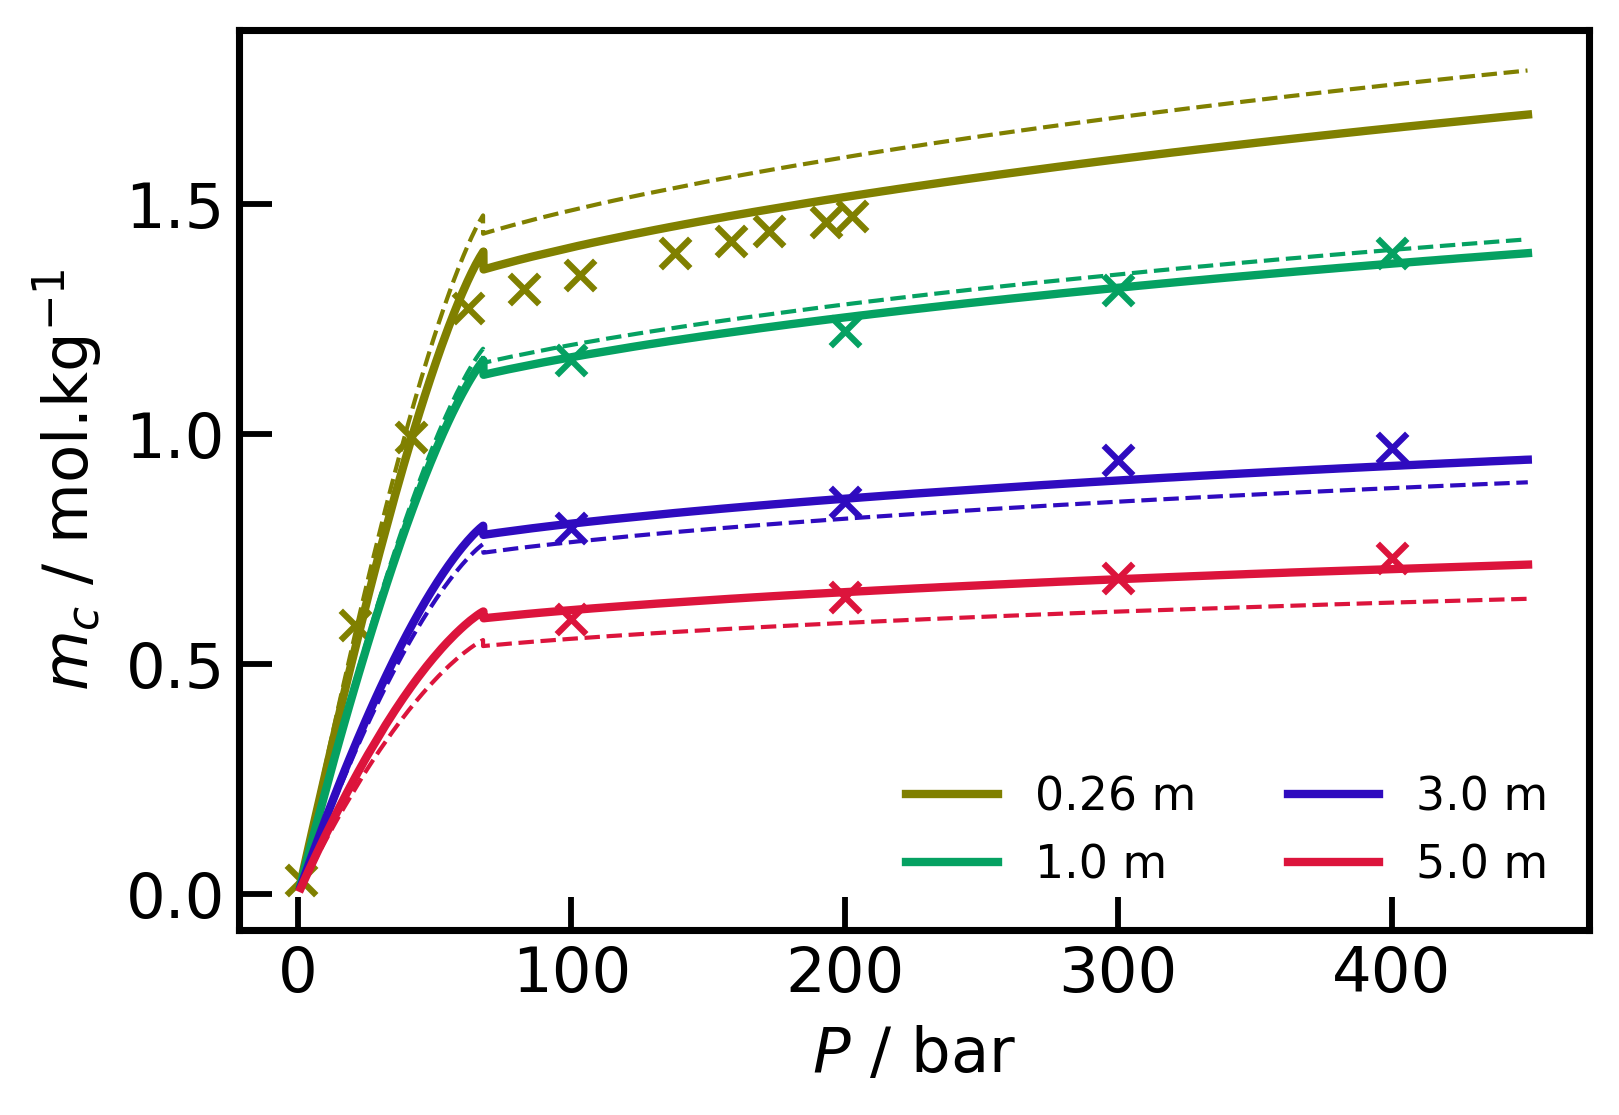
\includegraphics[width=.98\linewidth]{Figures/mcW_TWvsDTU_T298K.png}
  \caption{$T$ = 298 K}
\end{subfigure}%
\begin{subfigure}{.33\textwidth}
  \centering
  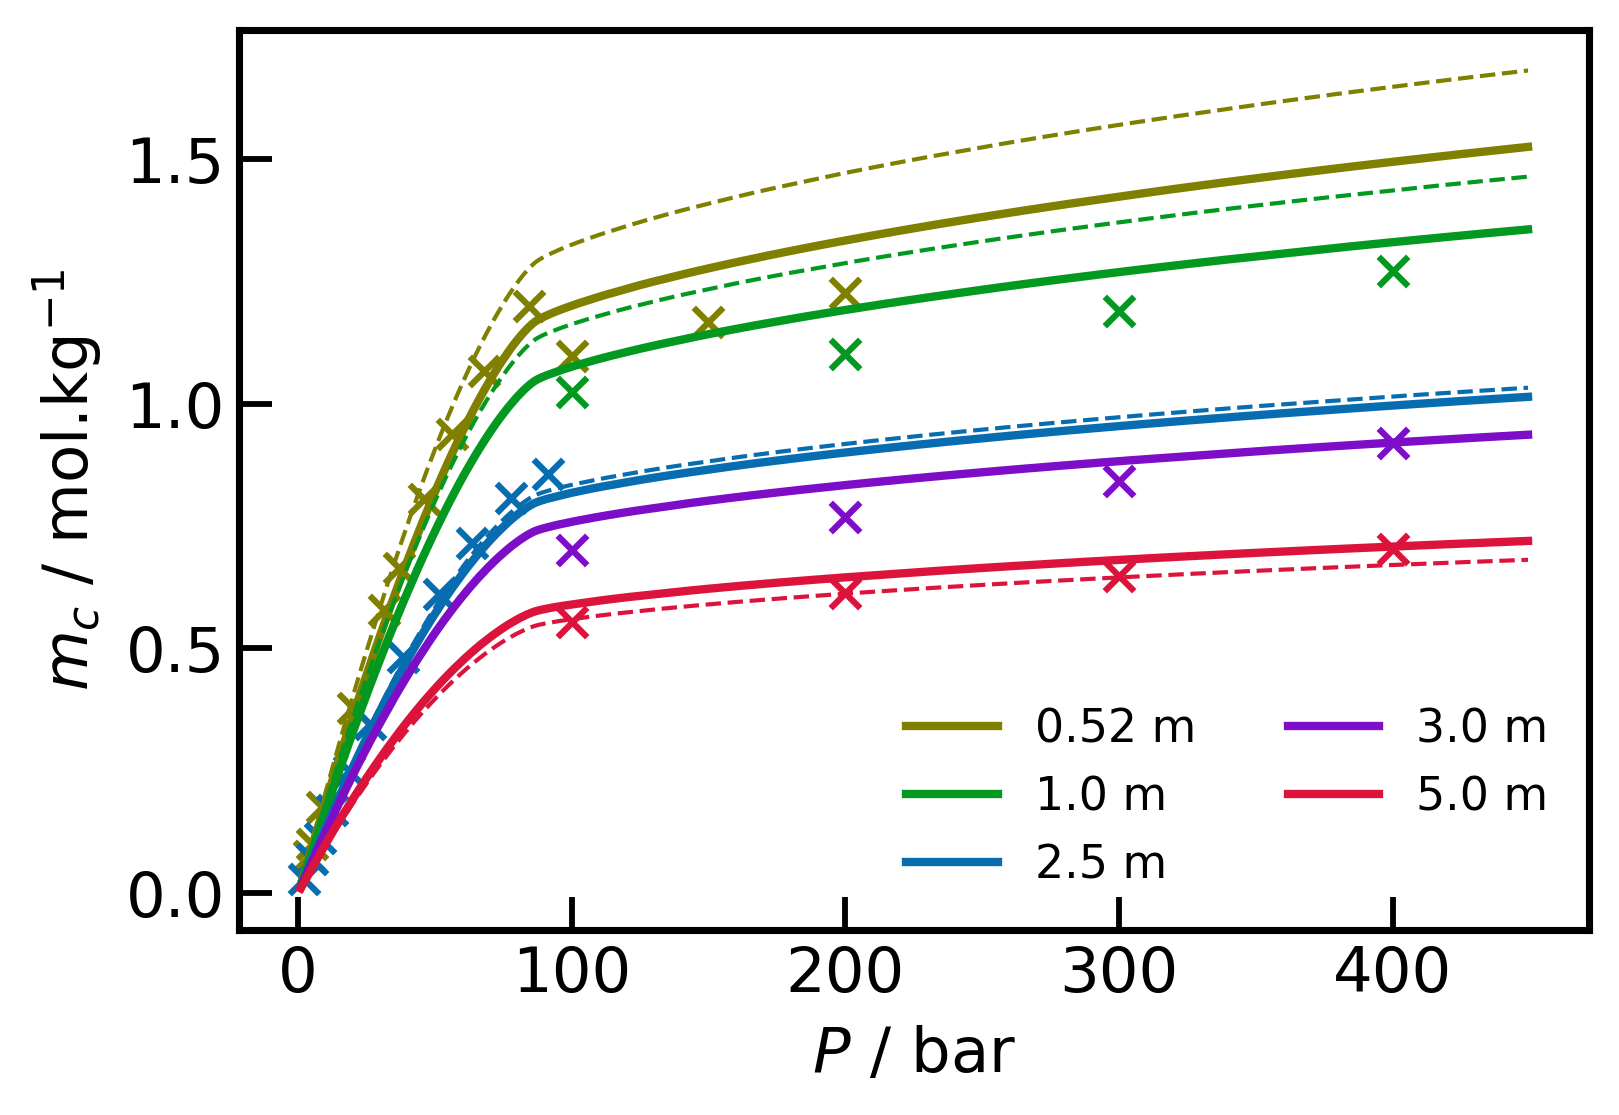
\includegraphics[width=.98\linewidth]{Figures/mcW_TWvsDTU_T313K.png}
  \caption{$T$ = 313 K}
\end{subfigure}%
\begin{subfigure}{.33\textwidth}
  \centering
  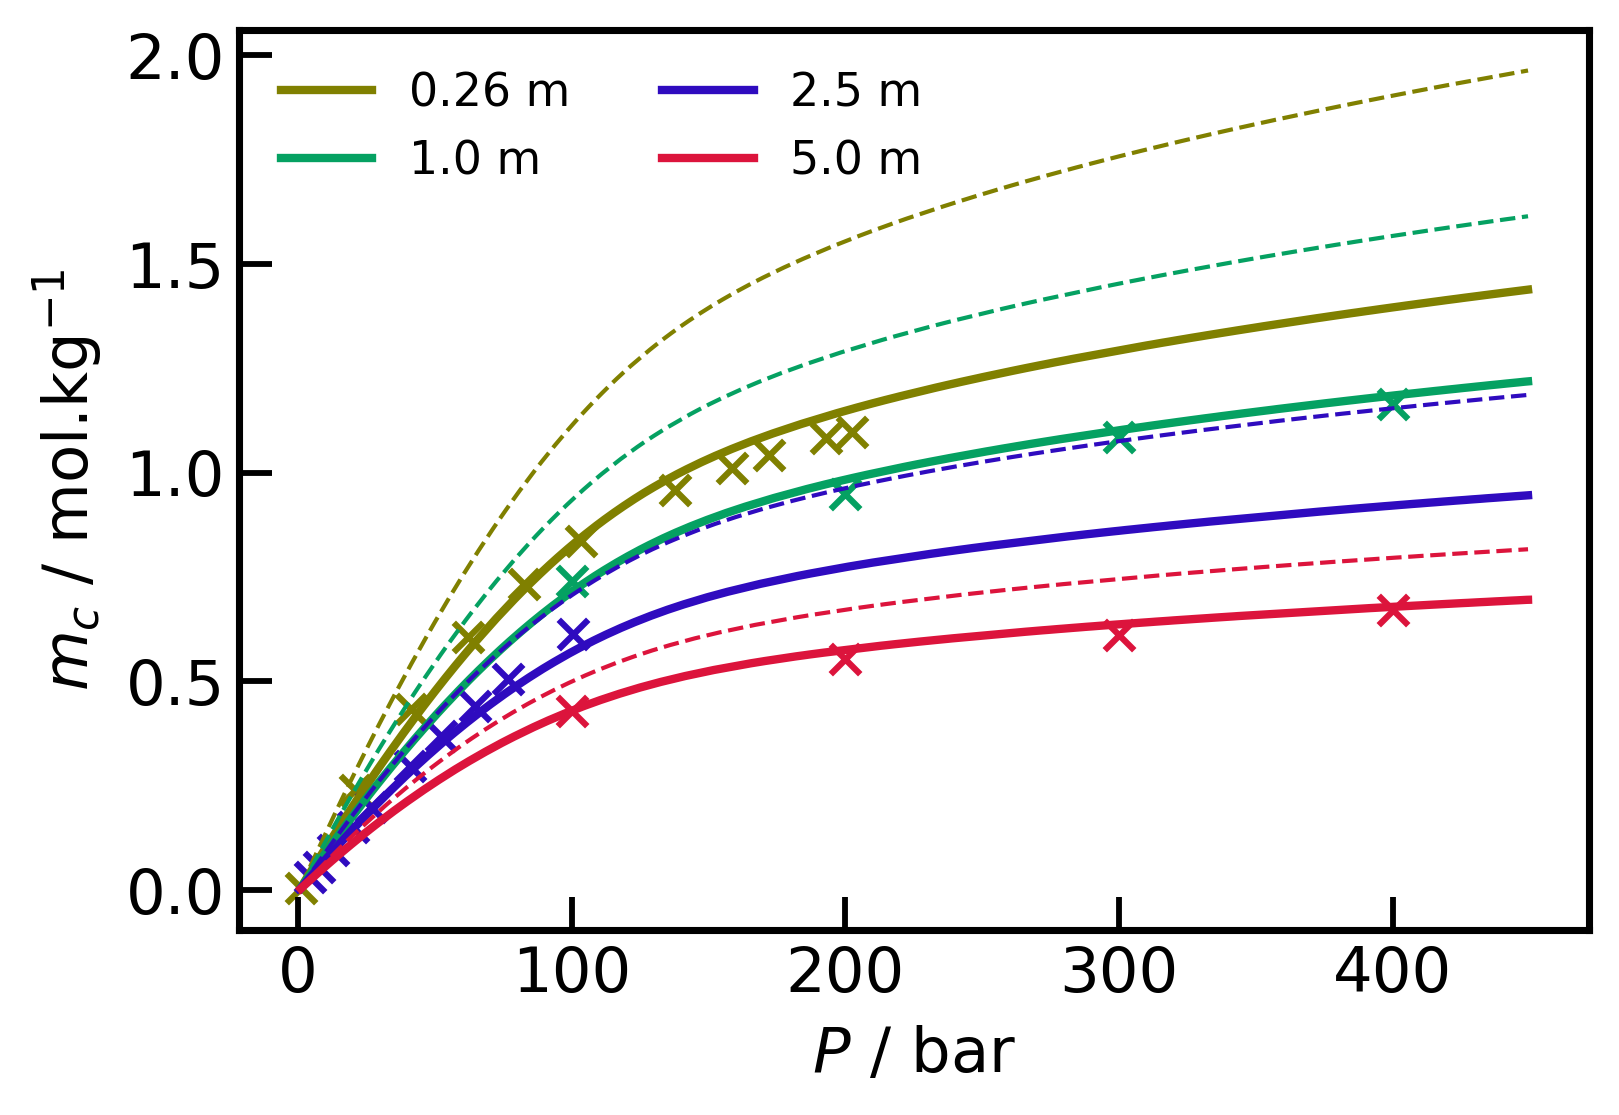
\includegraphics[width=.98\linewidth]{Figures/mcW_TWvsDTU_T353K.png}
  \caption{$T$ = 353 K}
\end{subfigure}%
\vskip\baselineskip
\begin{subfigure}{.33\textwidth}
  \centering
  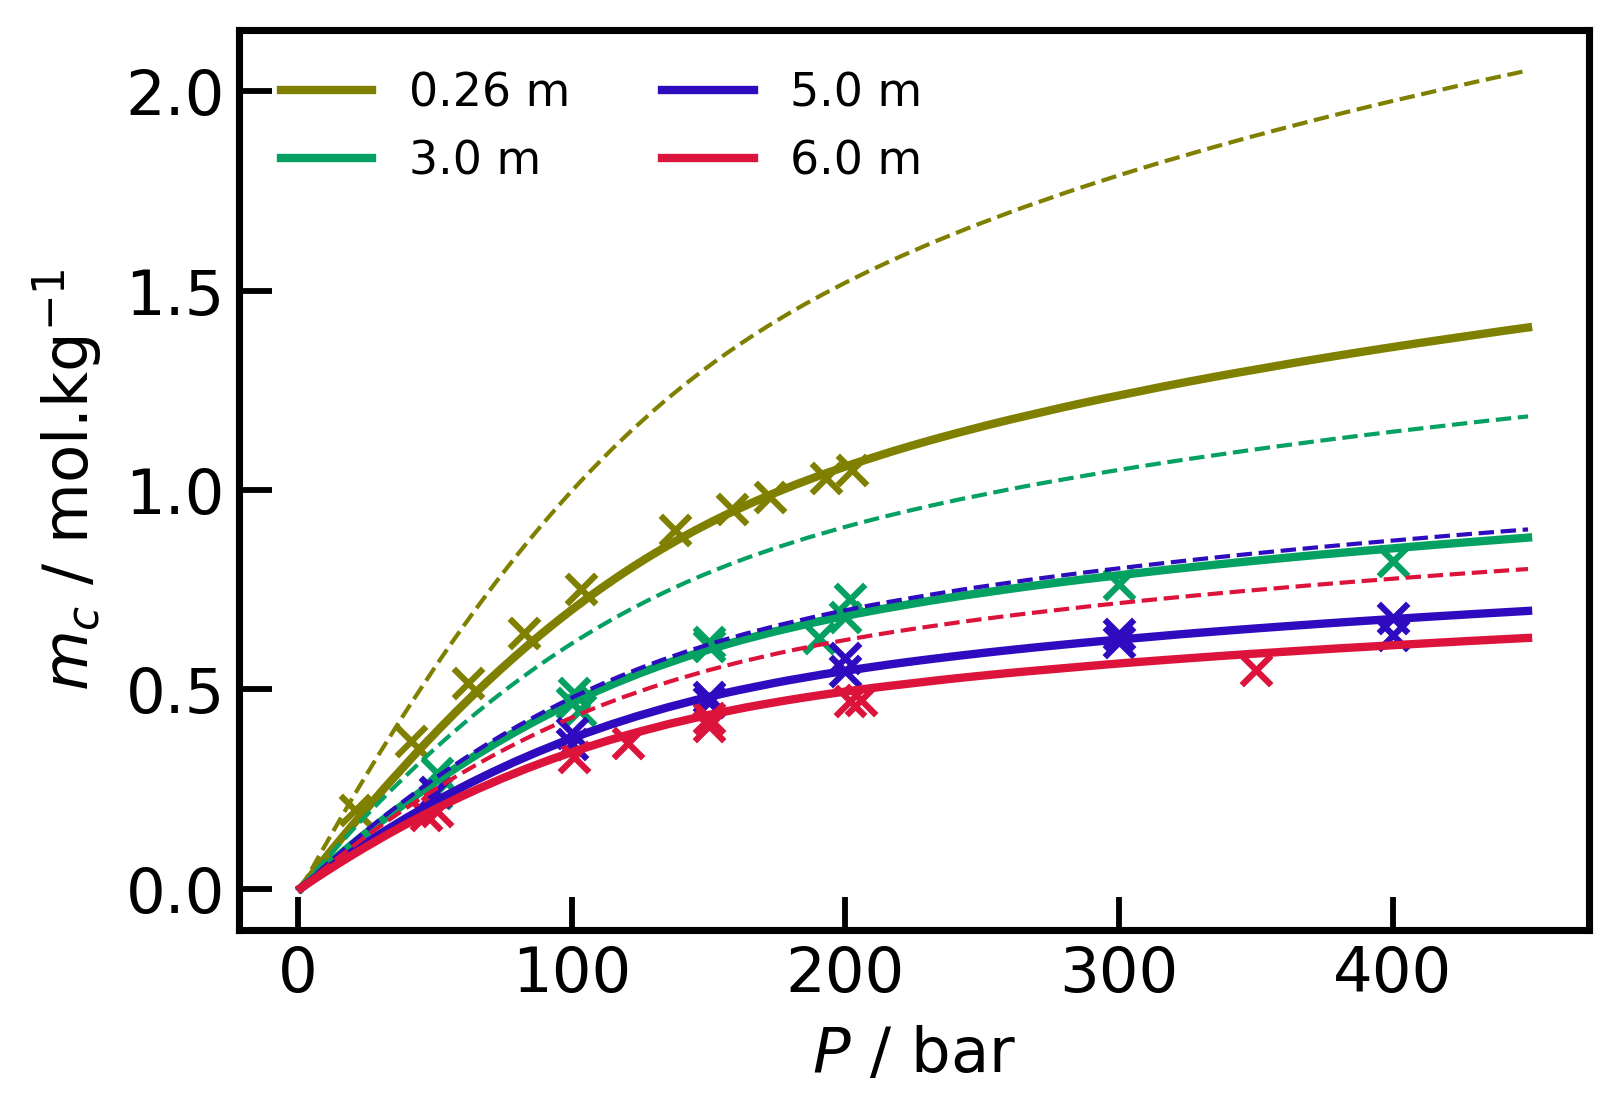
\includegraphics[width=.98\linewidth]{Figures/mcW_TWvsDTU_T373K.png}
  \caption{$T$ = 373 K}
\end{subfigure}%
\begin{subfigure}{.33\textwidth}
  \centering
  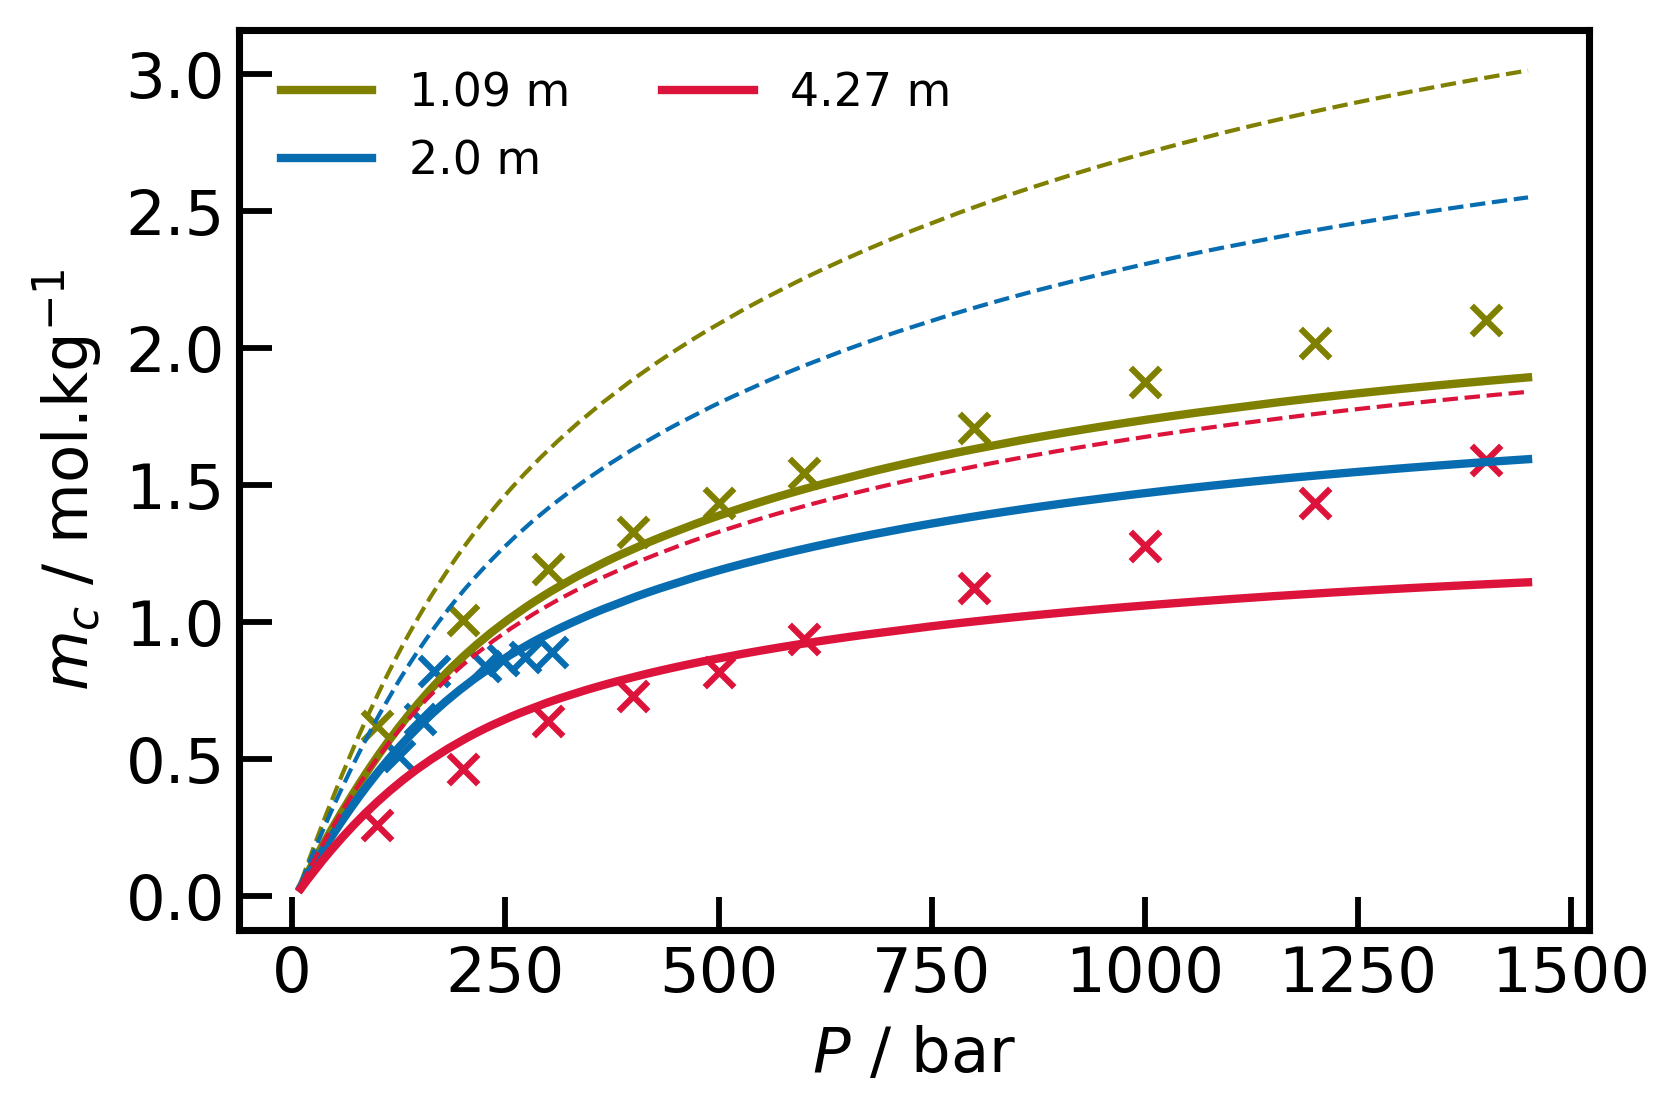
\includegraphics[width=.98\linewidth]{Figures/mcW_TWvsDTU_T423K.png}
  \caption{$T$ = 423 K}
\end{subfigure}%
\begin{subfigure}{.33\textwidth}
  \centering
  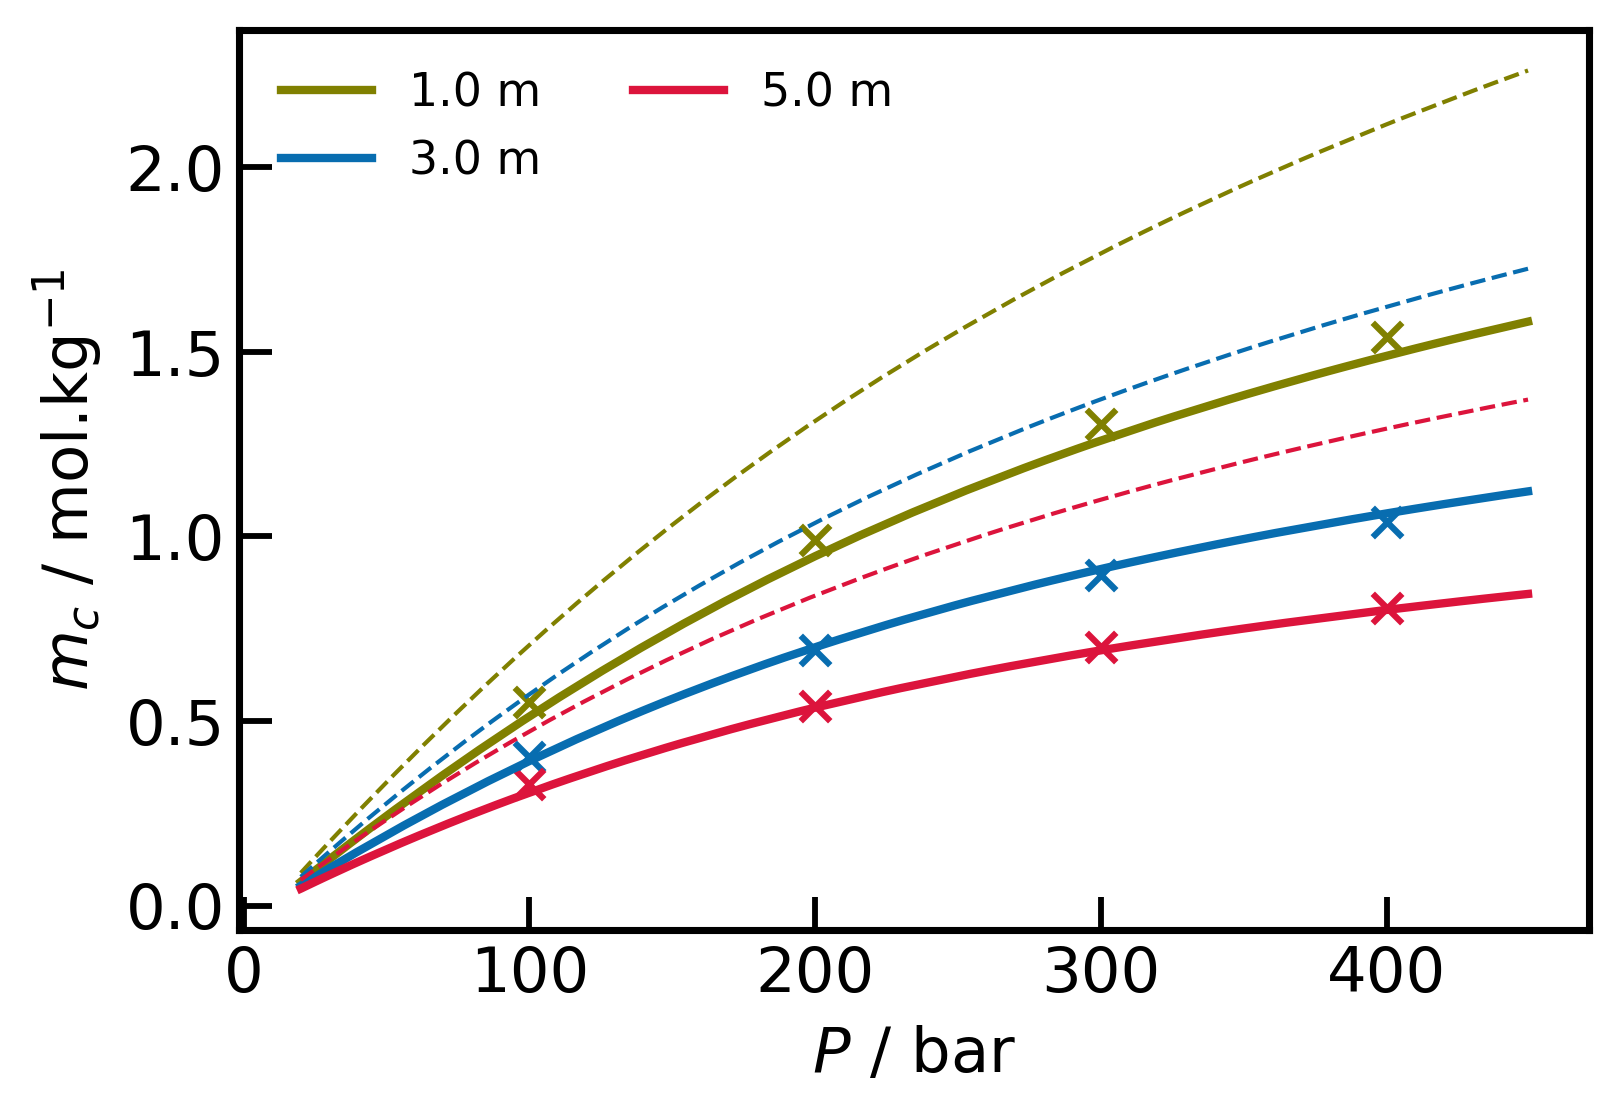
\includegraphics[width=.98\linewidth]{Figures/mcW_TWvsDTU_T453K.png}
  \caption{$T$ = 453 K}
\end{subfigure}%
\vskip\baselineskip
\begin{subfigure}{.33\textwidth}
  \centering
  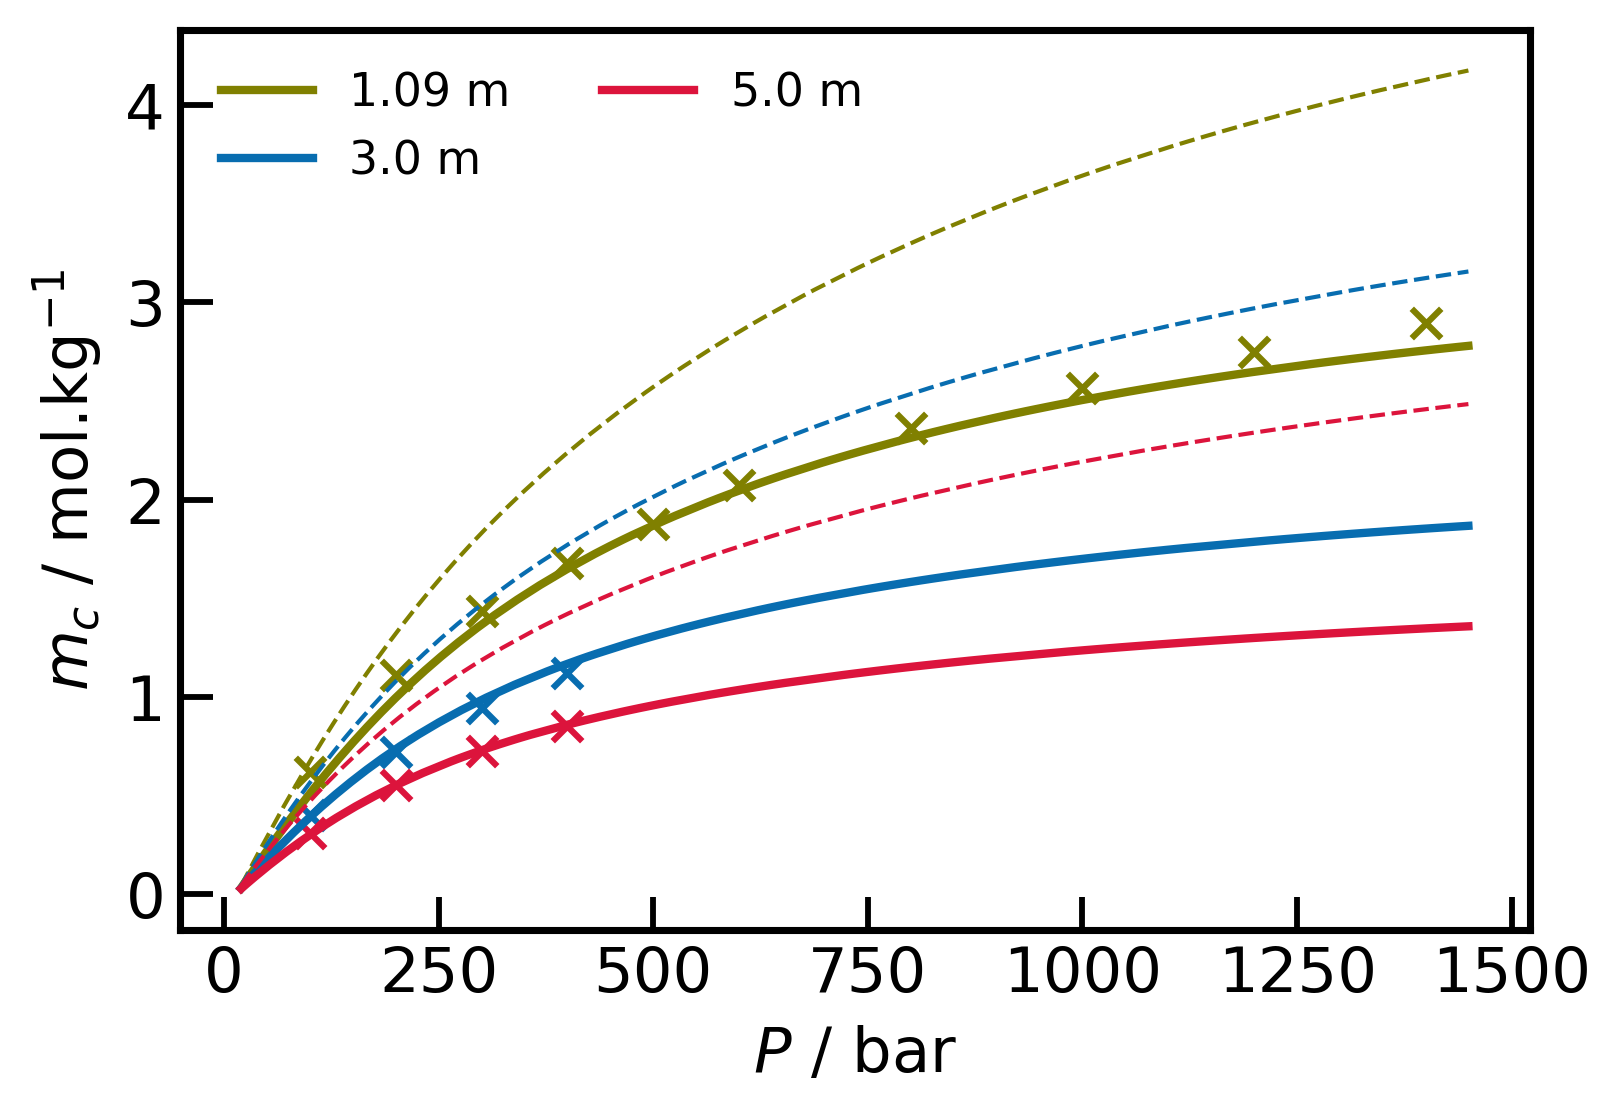
\includegraphics[width=.98\linewidth]{Figures/mcW_TWvsDTU_T473K.png}
  \caption{$T$ = 473 K}
\end{subfigure}%
\begin{subfigure}{.33\textwidth}
  \centering
  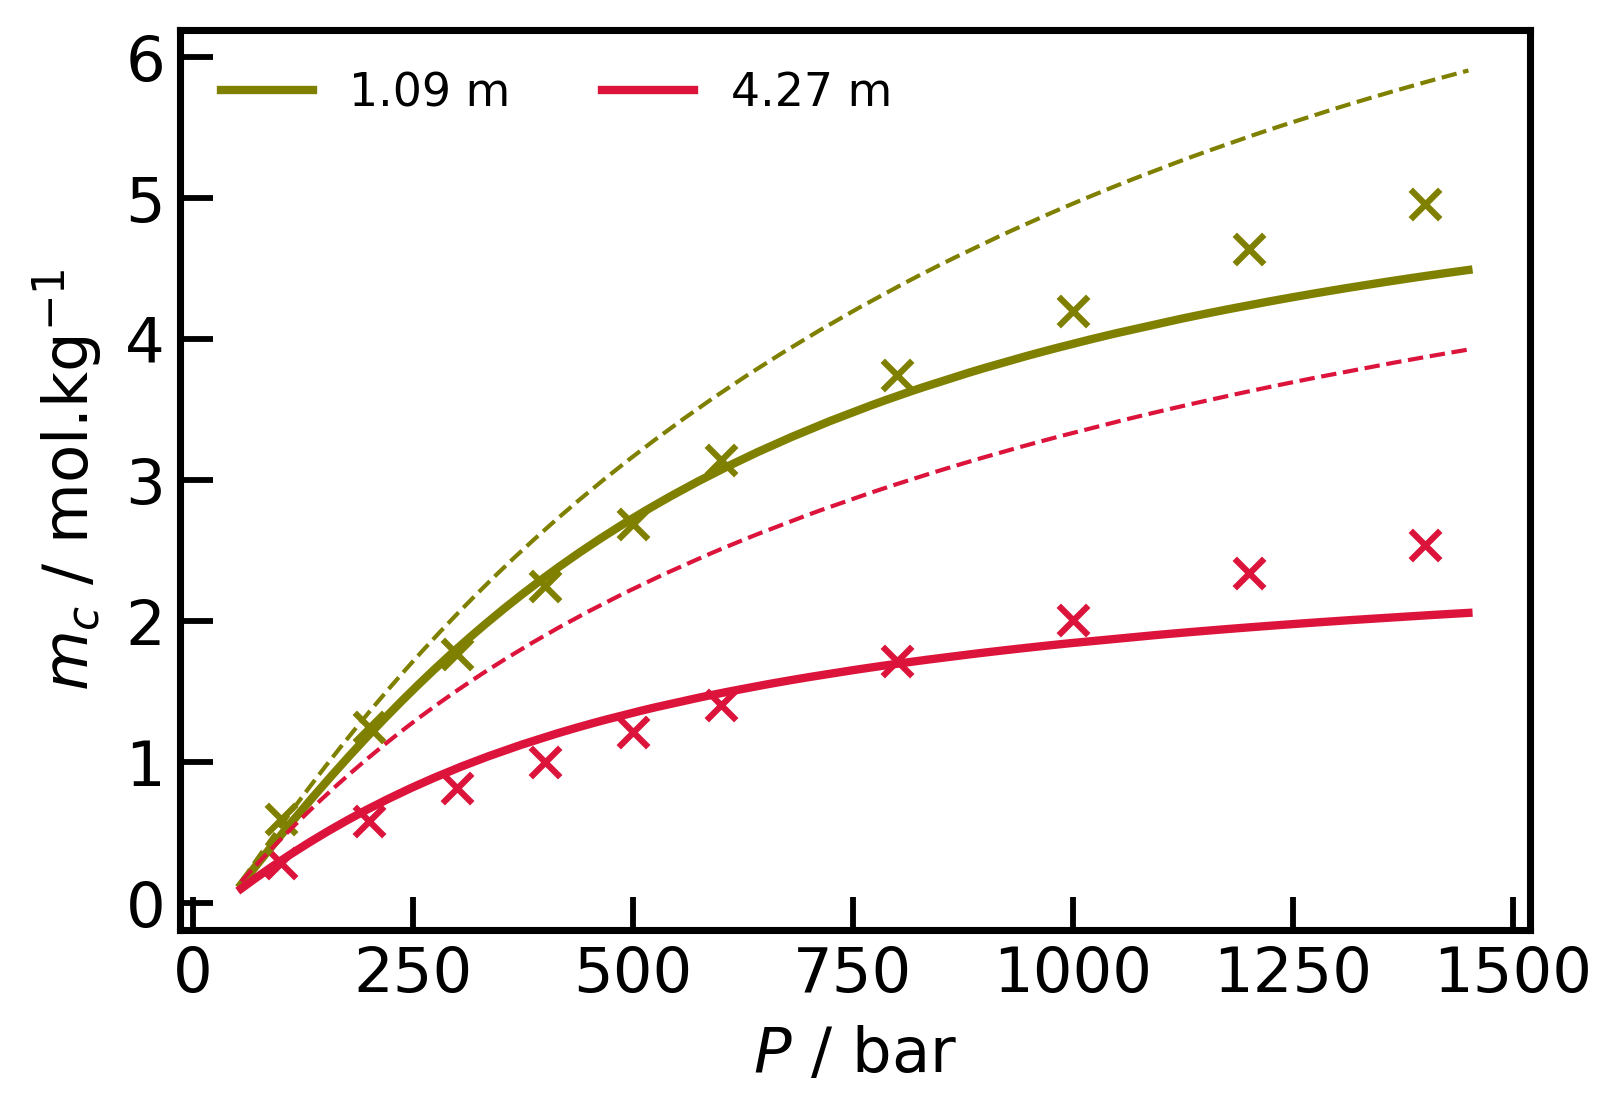
\includegraphics[width=.98\linewidth]{Figures/mcW_TWvsDTU_T523K.png}
  \caption{$T$ = 523 K}
\end{subfigure}%
\begin{subfigure}{.33\textwidth}
  \centering
  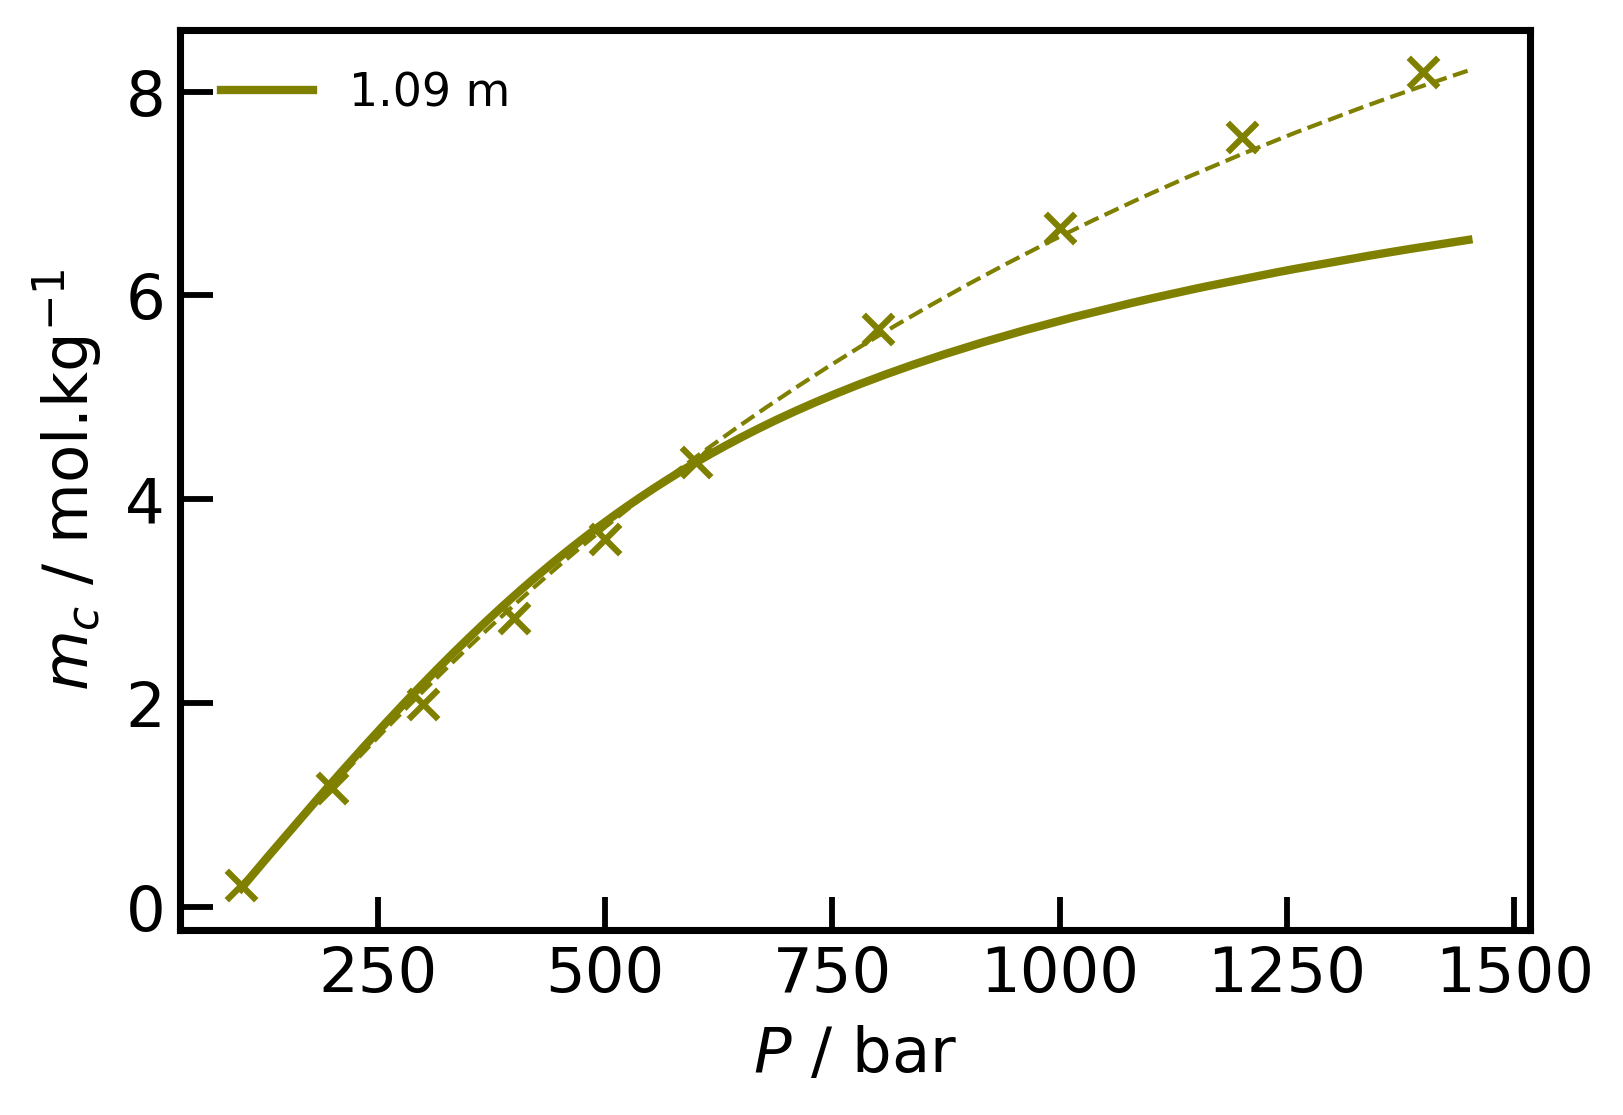
\includegraphics[width=.98\linewidth]{Figures/mcW_TWvsDTU_T573K.png}
  \caption{$T$ = 573 K}
\end{subfigure}%
\vskip\baselineskip
\begin{subfigure}{.33\textwidth}
  \centering
  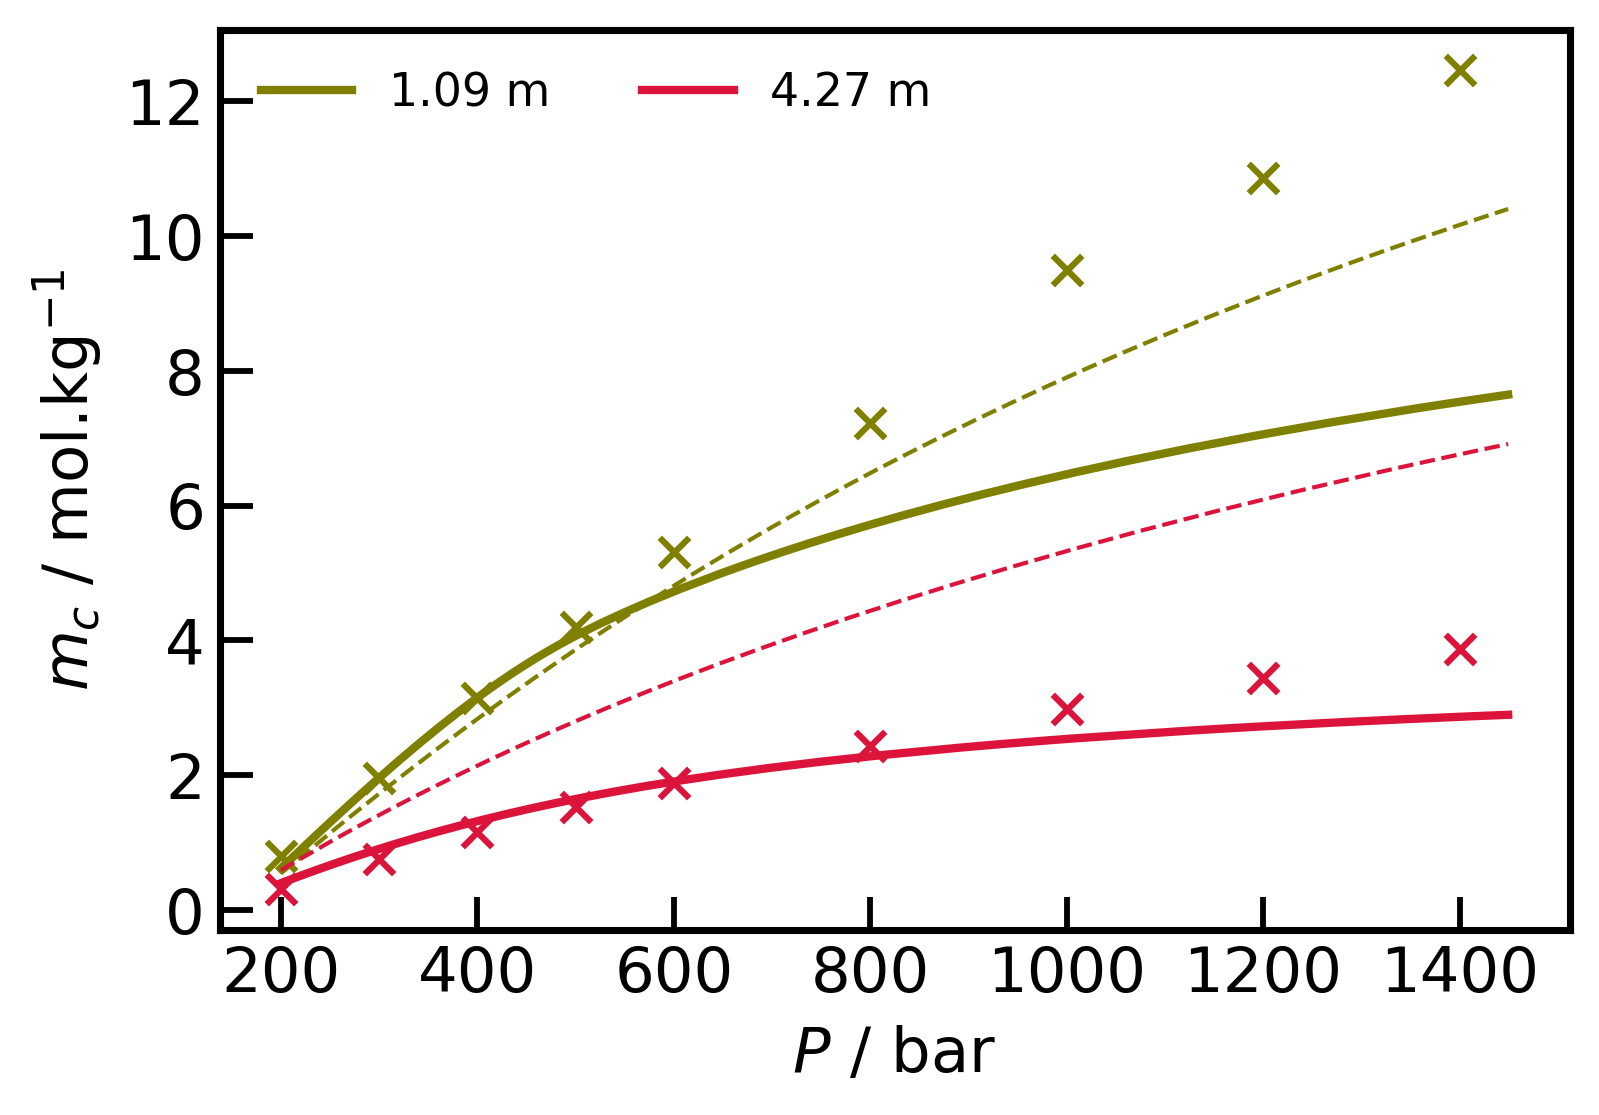
\includegraphics[width=.98\linewidth]{Figures/mcW_TWvsDTU_T623K.png}
  \caption{$T$ = 623 K}
\end{subfigure}%
\begin{subfigure}{.33\textwidth}
  \centering
  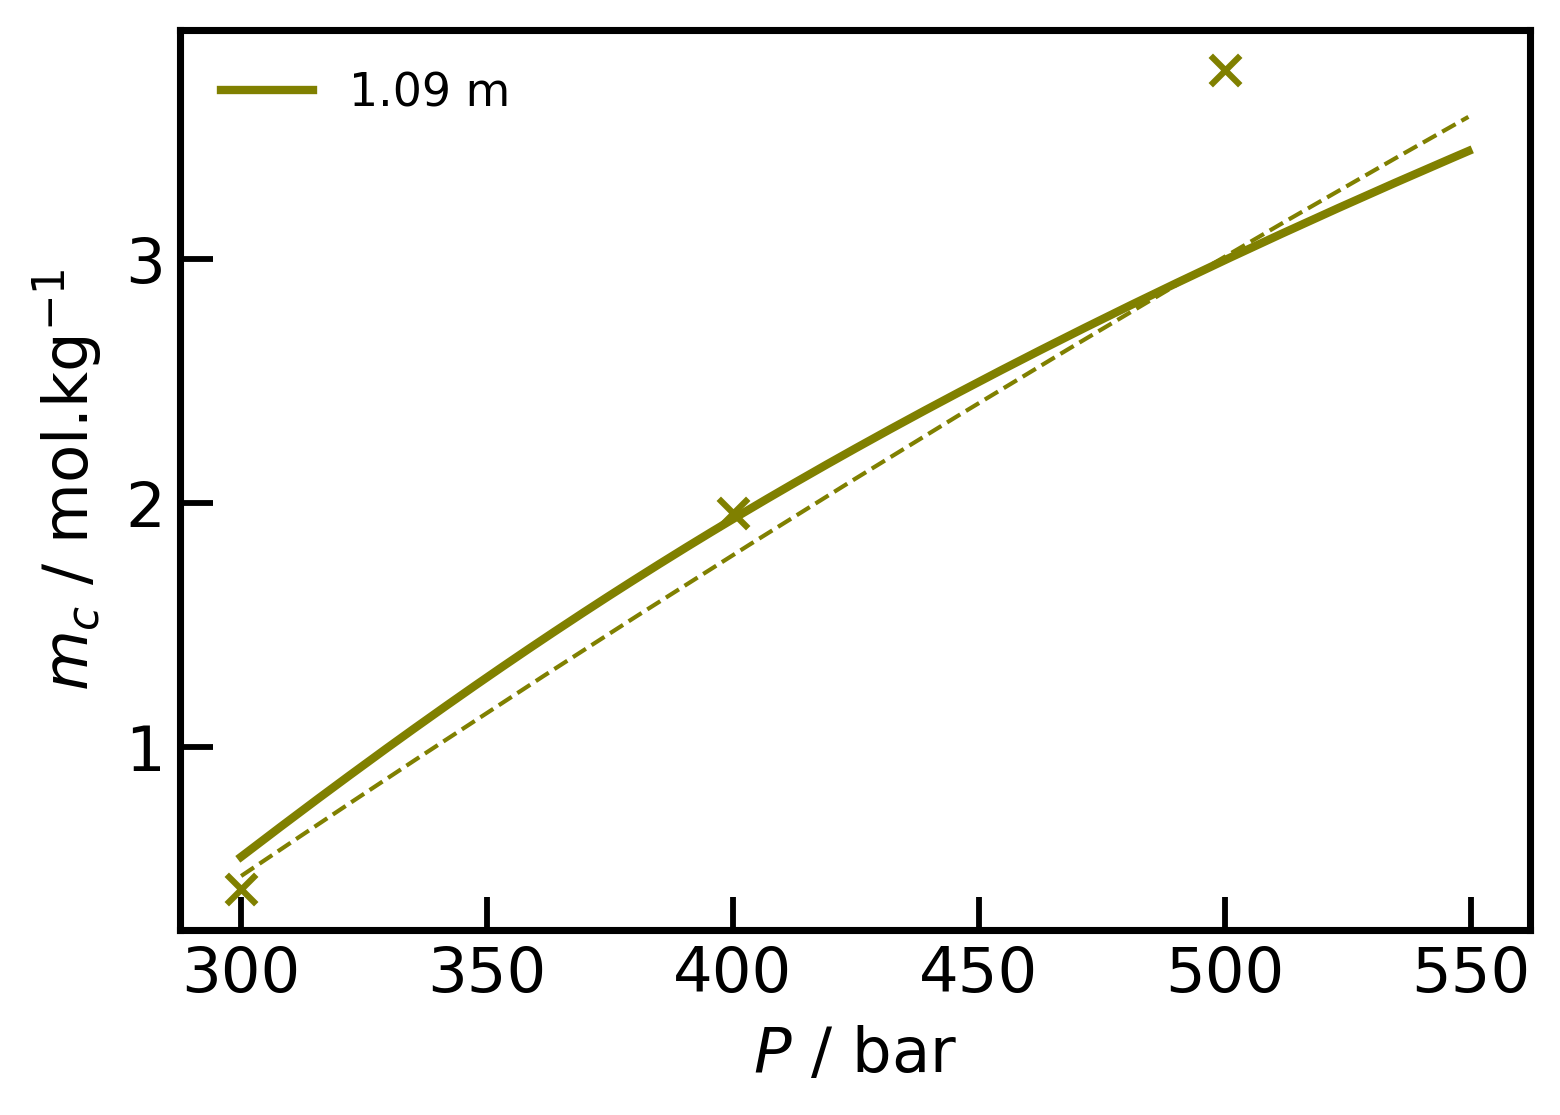
\includegraphics[width=.98\linewidth]{Figures/mcW_TWvsDTU_T673K.png}
  \caption{$T$ = 673 K}
\end{subfigure}%
\begin{subfigure}{.33\textwidth}
  \centering
  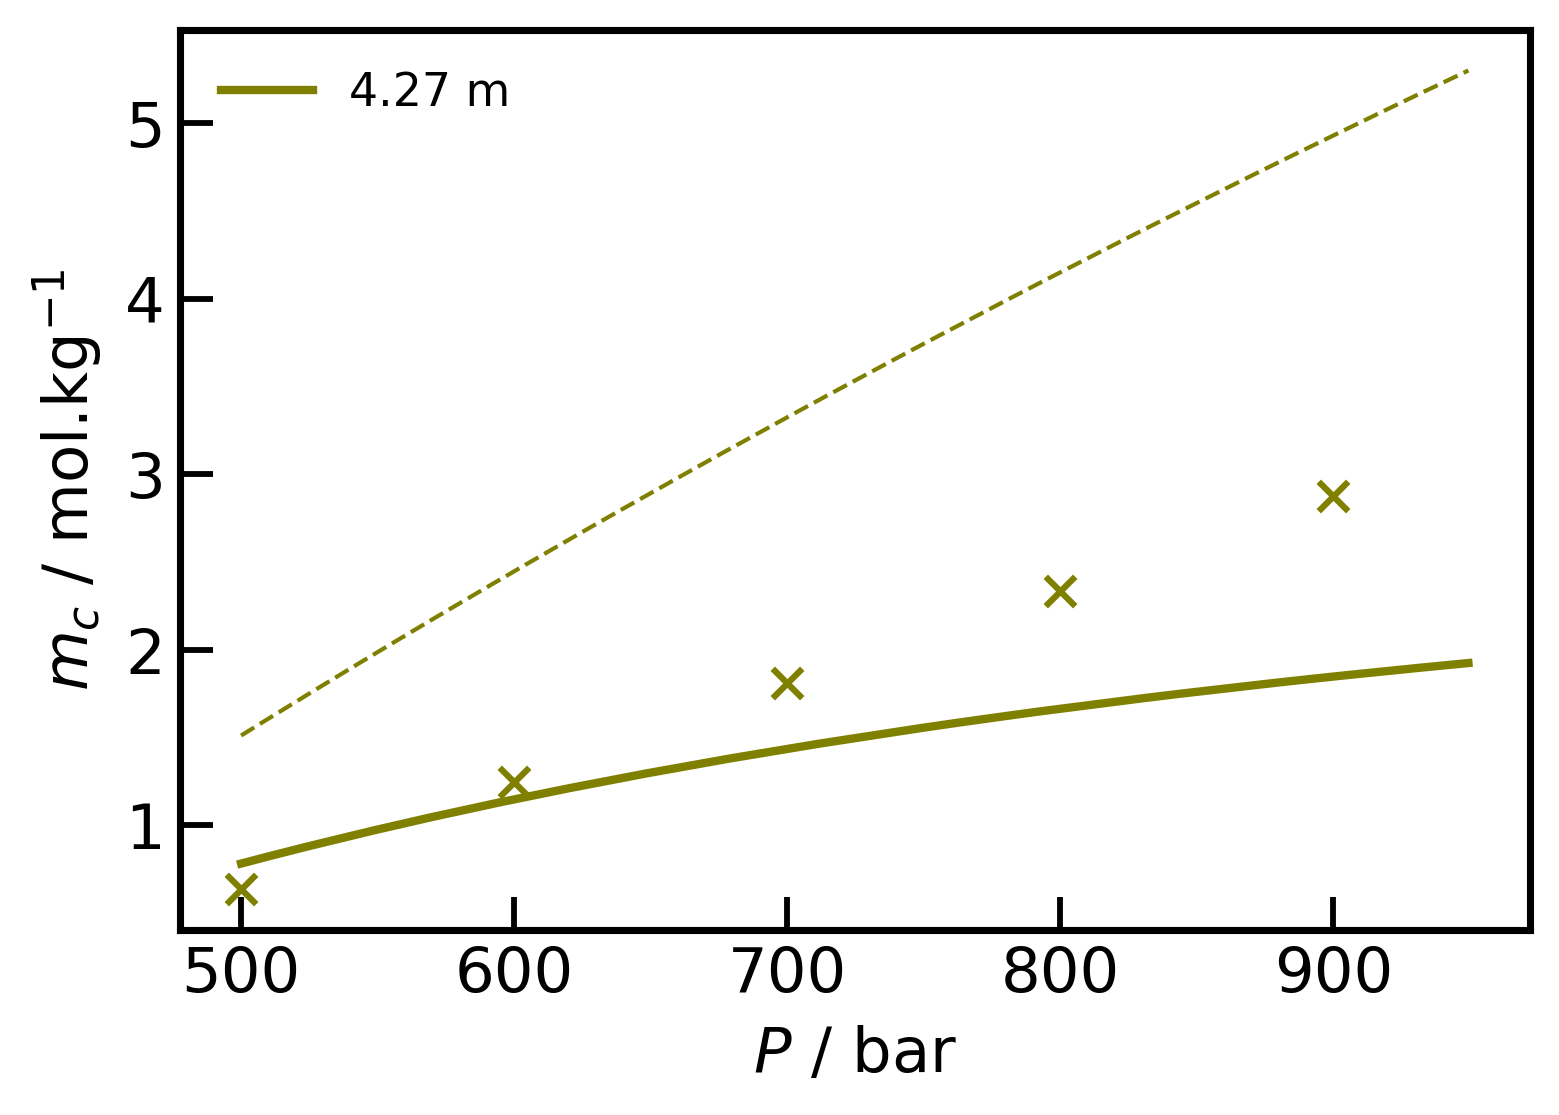
\includegraphics[width=.98\linewidth]{Figures/mcW_TWvsDTU_T723K.png}
  \caption{$T$ = 723 K}
\end{subfigure}%
\vskip\baselineskip
\label{CB_TW_DTU}
\caption{\ce{CO2} solubility in NaCl brine at various temperatures (a-l) from eCPA models (This Work in continuous lines and DTU \cite{Maribo2015} in dashed lines) and experiments \cite{Guo2016, Liu2021, Bando2003, Chabab2019, Kiepe2002, Rumpf1994, Hou2013, Koschel2006, Messabeb2016, Yan2011, Zhao2015, Nighswander1989, Savary2012, Takenouchi1965} (discrete points).}
\end{figure}

\newpage

\begin{figure}[h!]
\begin{subfigure}{.43\textwidth}
  \centering
  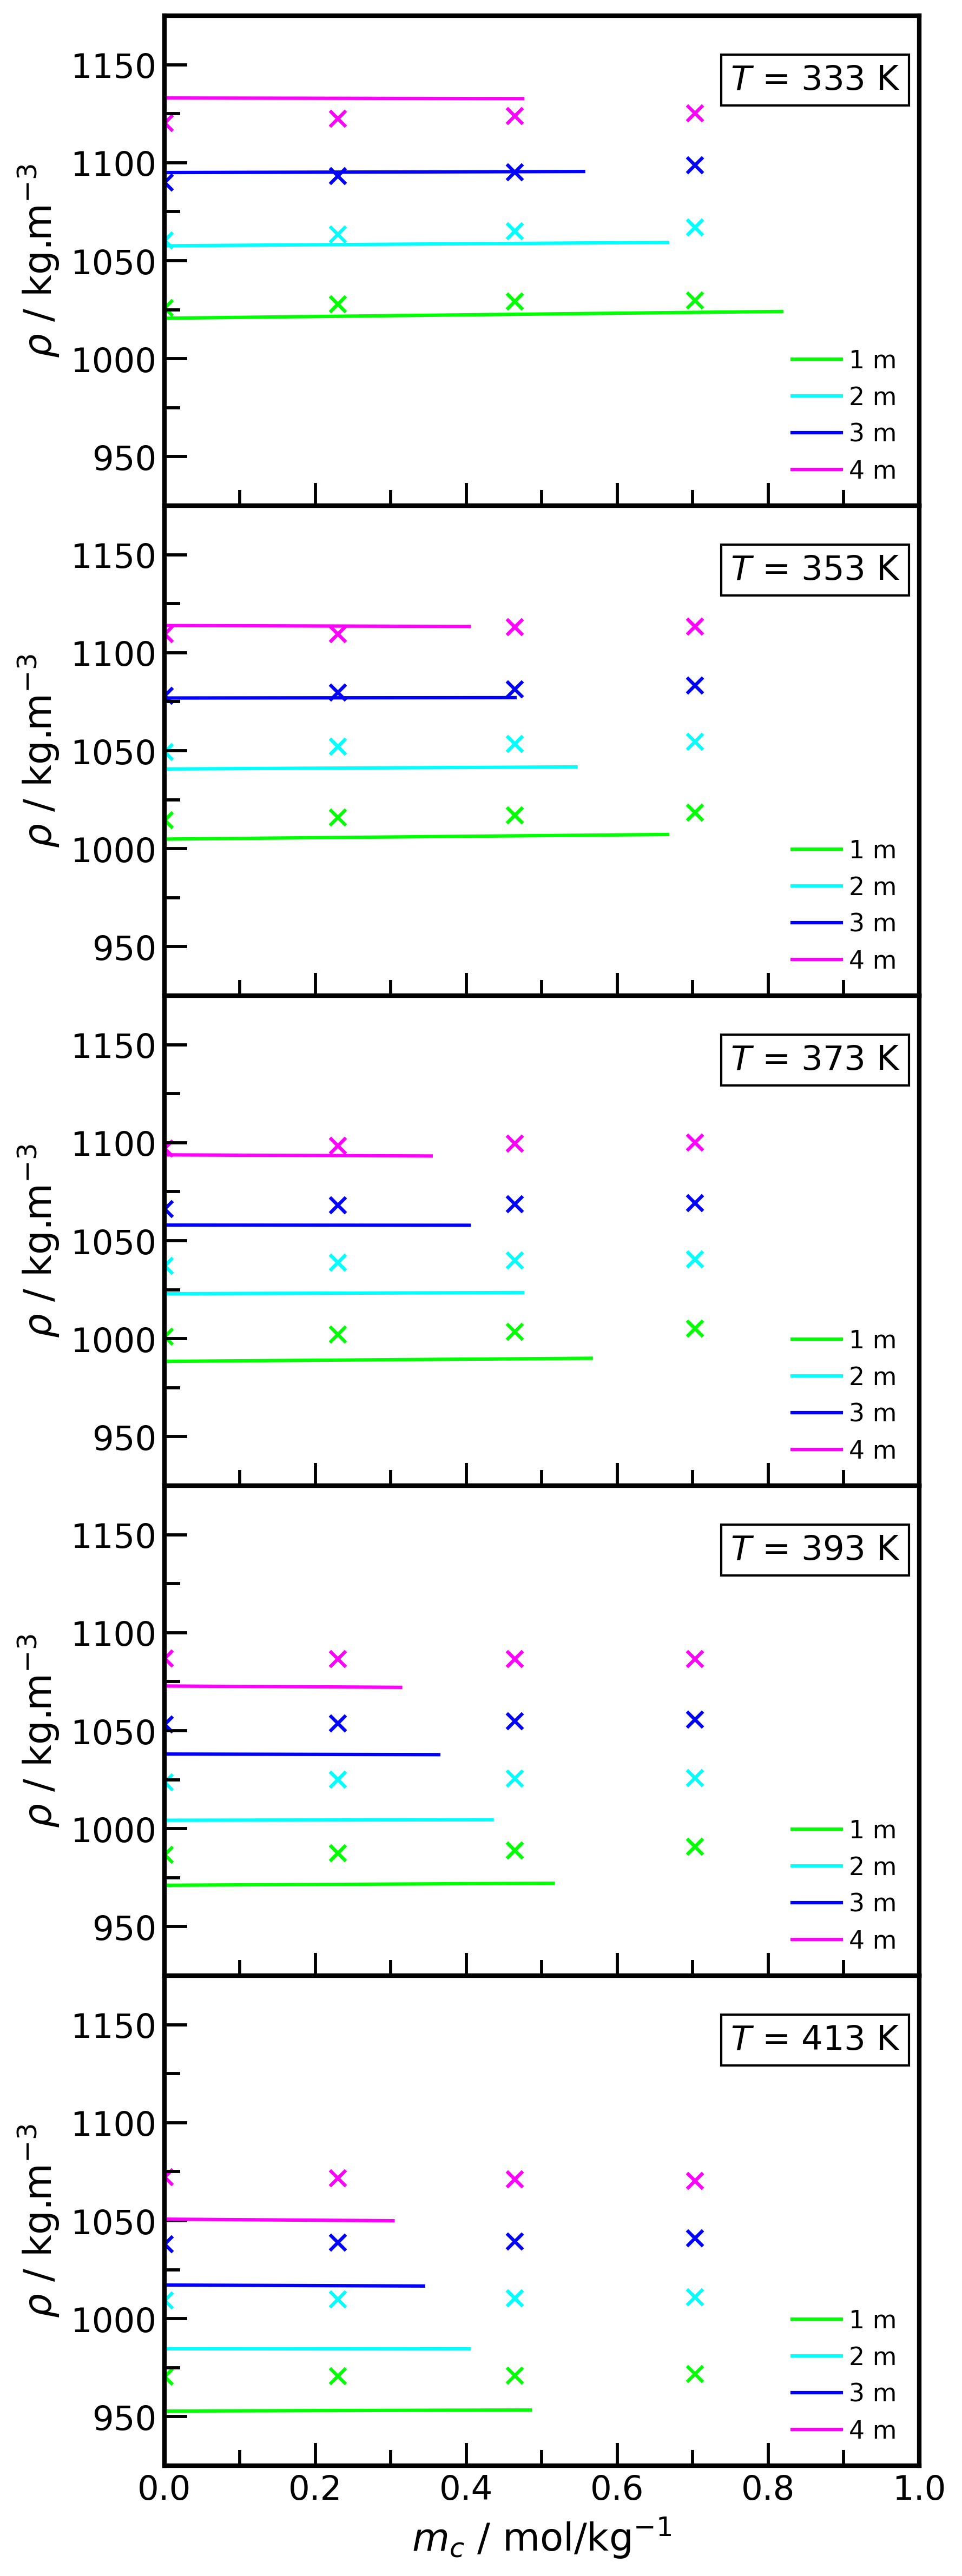
\includegraphics[width=.98\linewidth]{Figures/RHOCB_P100b.png}
  \caption{$P$ = 100 bar}
\end{subfigure}%
\begin{subfigure}{.43\textwidth}
  \centering
  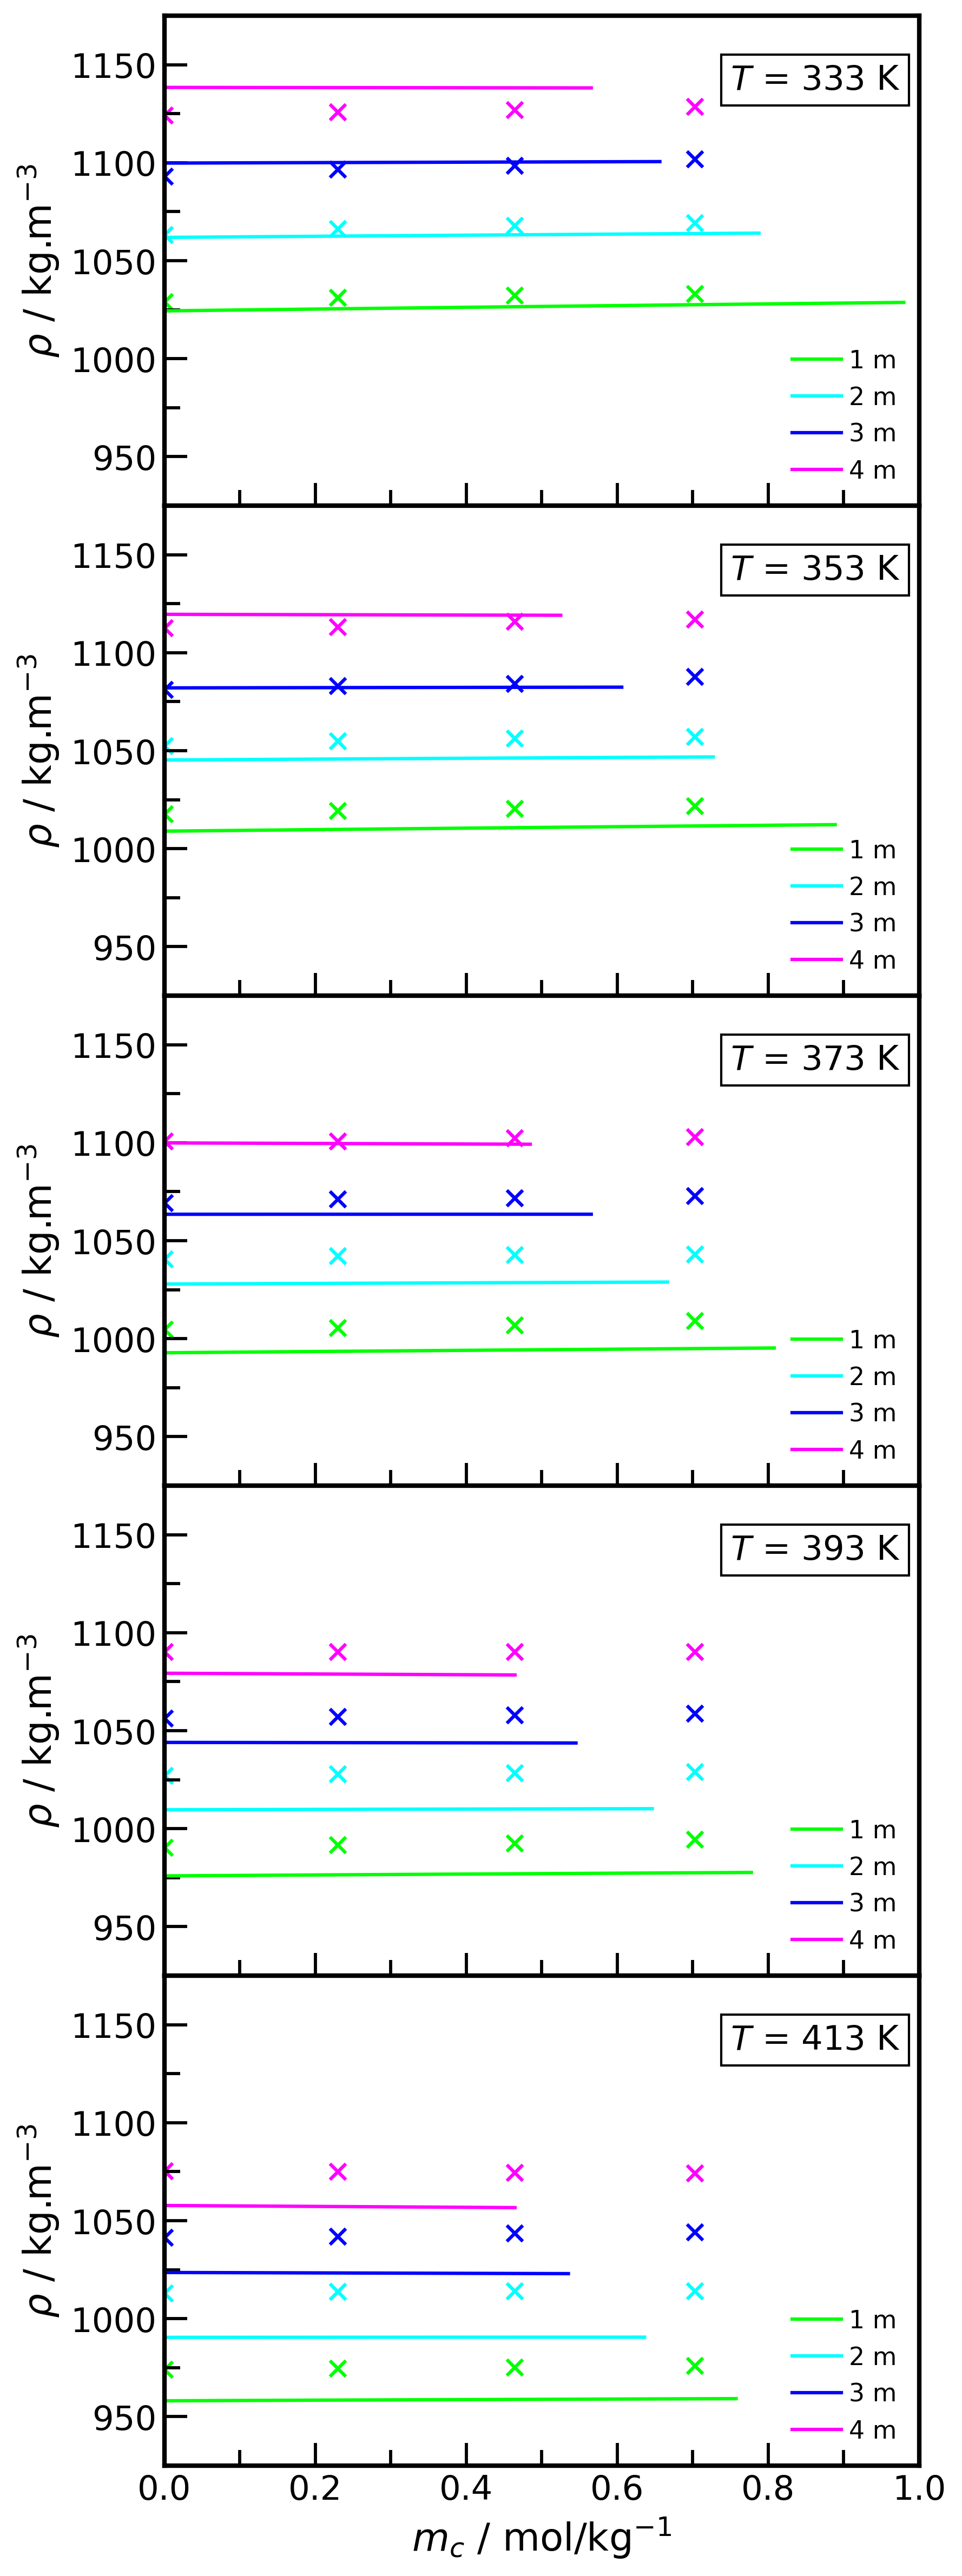
\includegraphics[width=.98\linewidth]{Figures/RHOCB_P180b.png}
  \caption{$P$ = 180 bar}
\end{subfigure}%
\label{CB_RHO}
\caption{Density of the aqueous phase in the \ce{CO2}-brine mixture below \ce{CO2} saturation \textit{vs.} \ce{CO2} concentration at various pressures, salinities and two different pressures (a-b) from eCPA EoS (continuous line) and experiments \cite{Song2013} (discrete points).}
\end{figure}

\newpage

\begin{figure}[h!]
\centering
  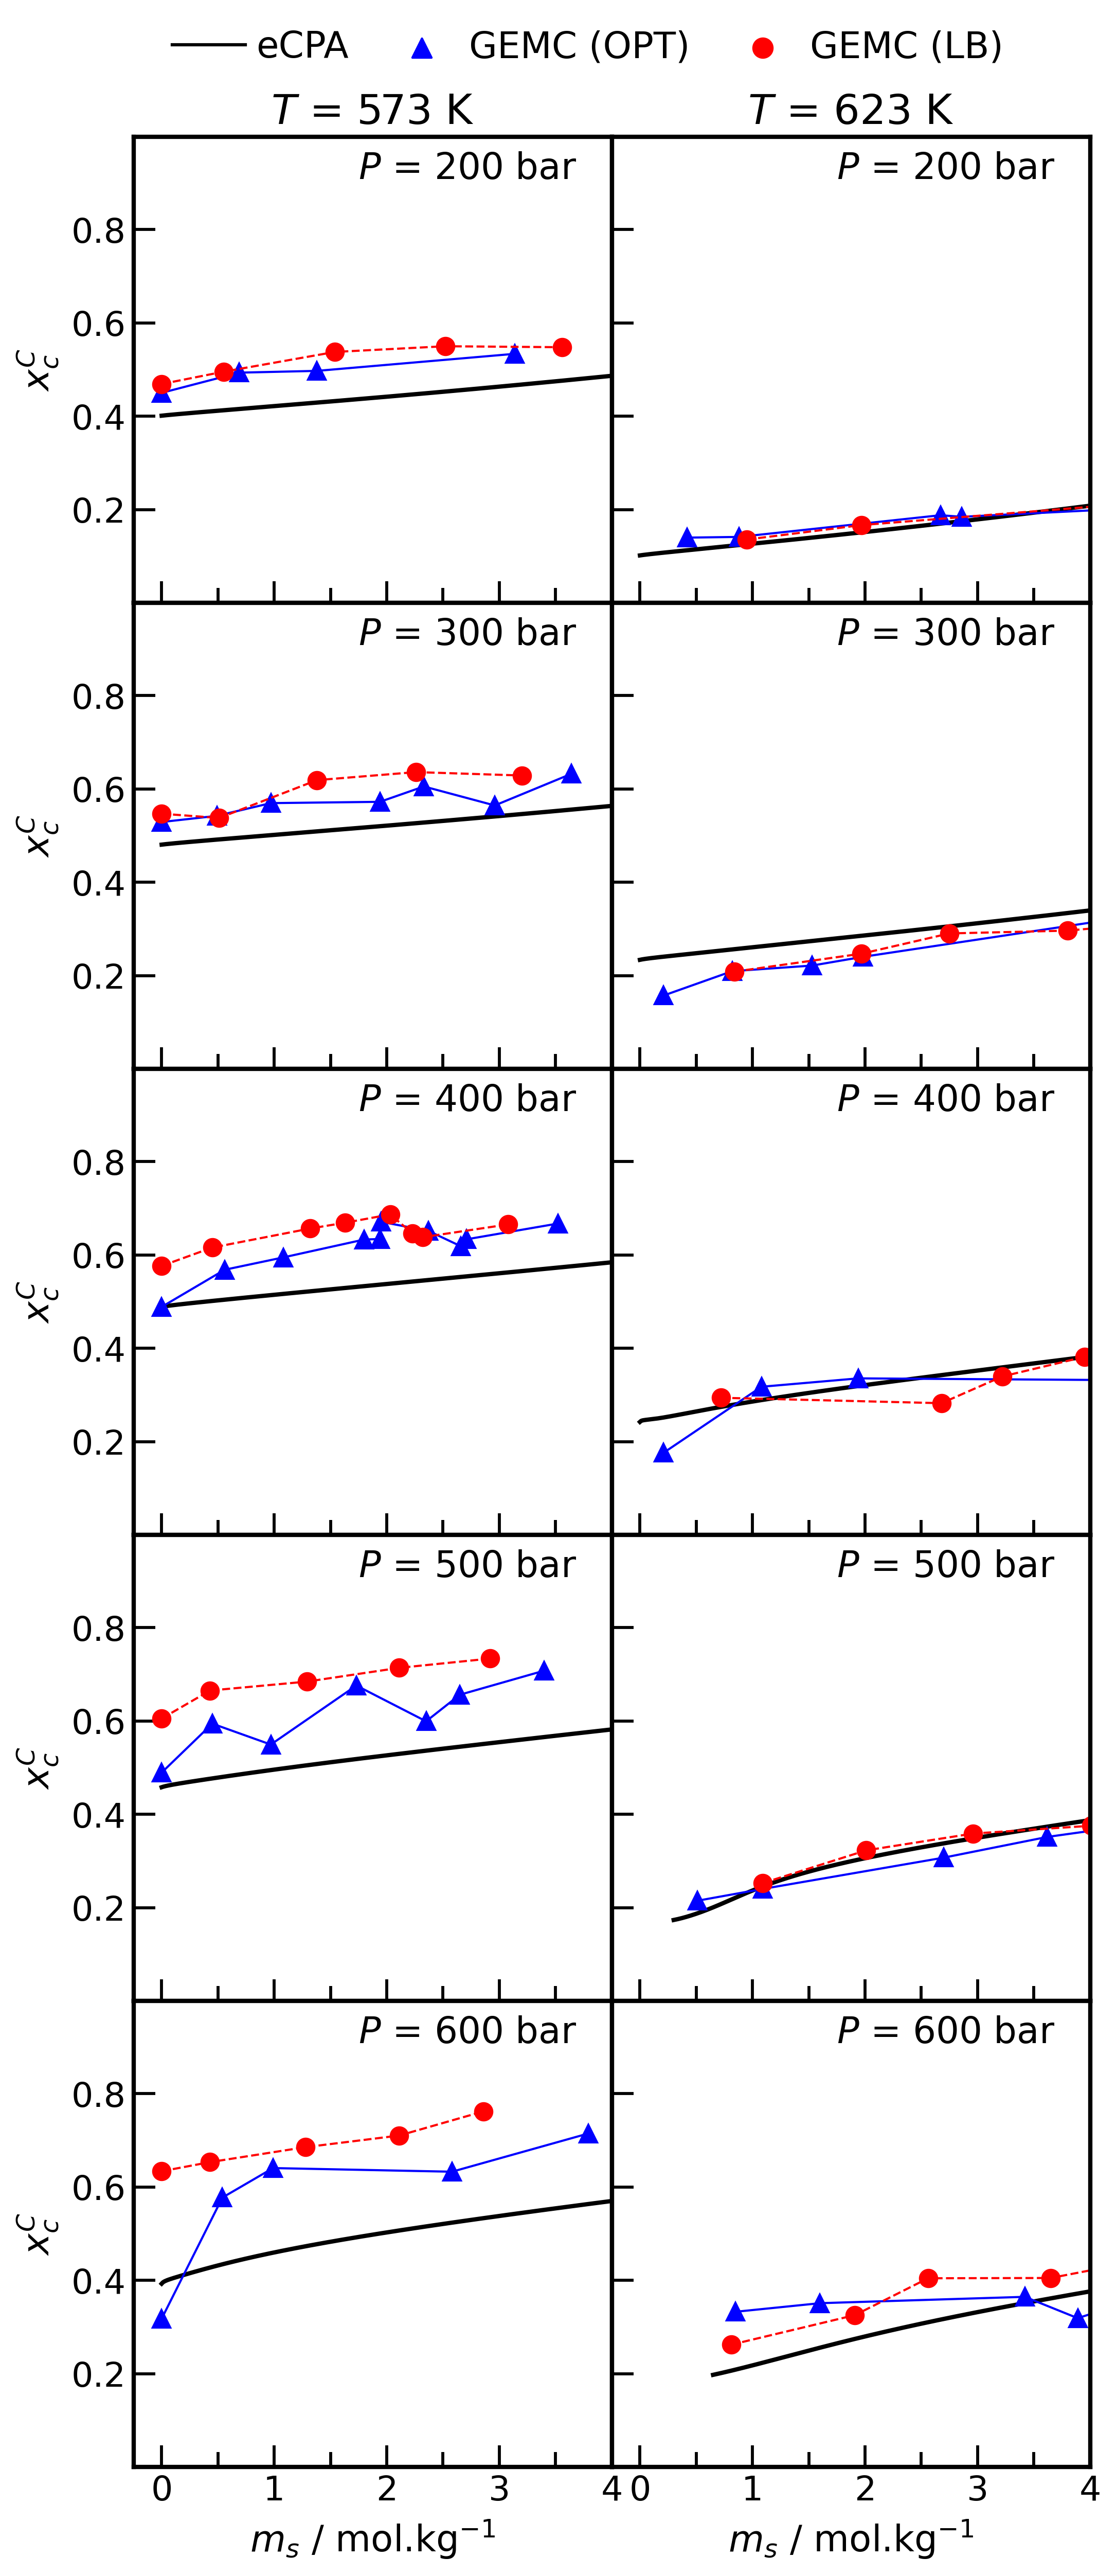
\includegraphics[width=0.5\textwidth]{Figures/GEMCvseCPA_xcC.png} 
\label{GEMC_CB_xcc}
\caption{\ce{CO2} solubility in the \ce{CO2}-rich phase in the \ce{CO2}-brine mixture \textit{vs.} salt concentration at various pressures and two different temperatures from GEMC simulations and eCPA EoS. "LB" and "OPT" stand for Lorentz-Berthelot and optimized (at lower temperatures \cite{Vlcek2011}) unlike parameters between \ce{CO2}-\ce{H2O} molecules, respectively.}
\end{figure}

\newpage



\begin{figure}[h!]
\centering
  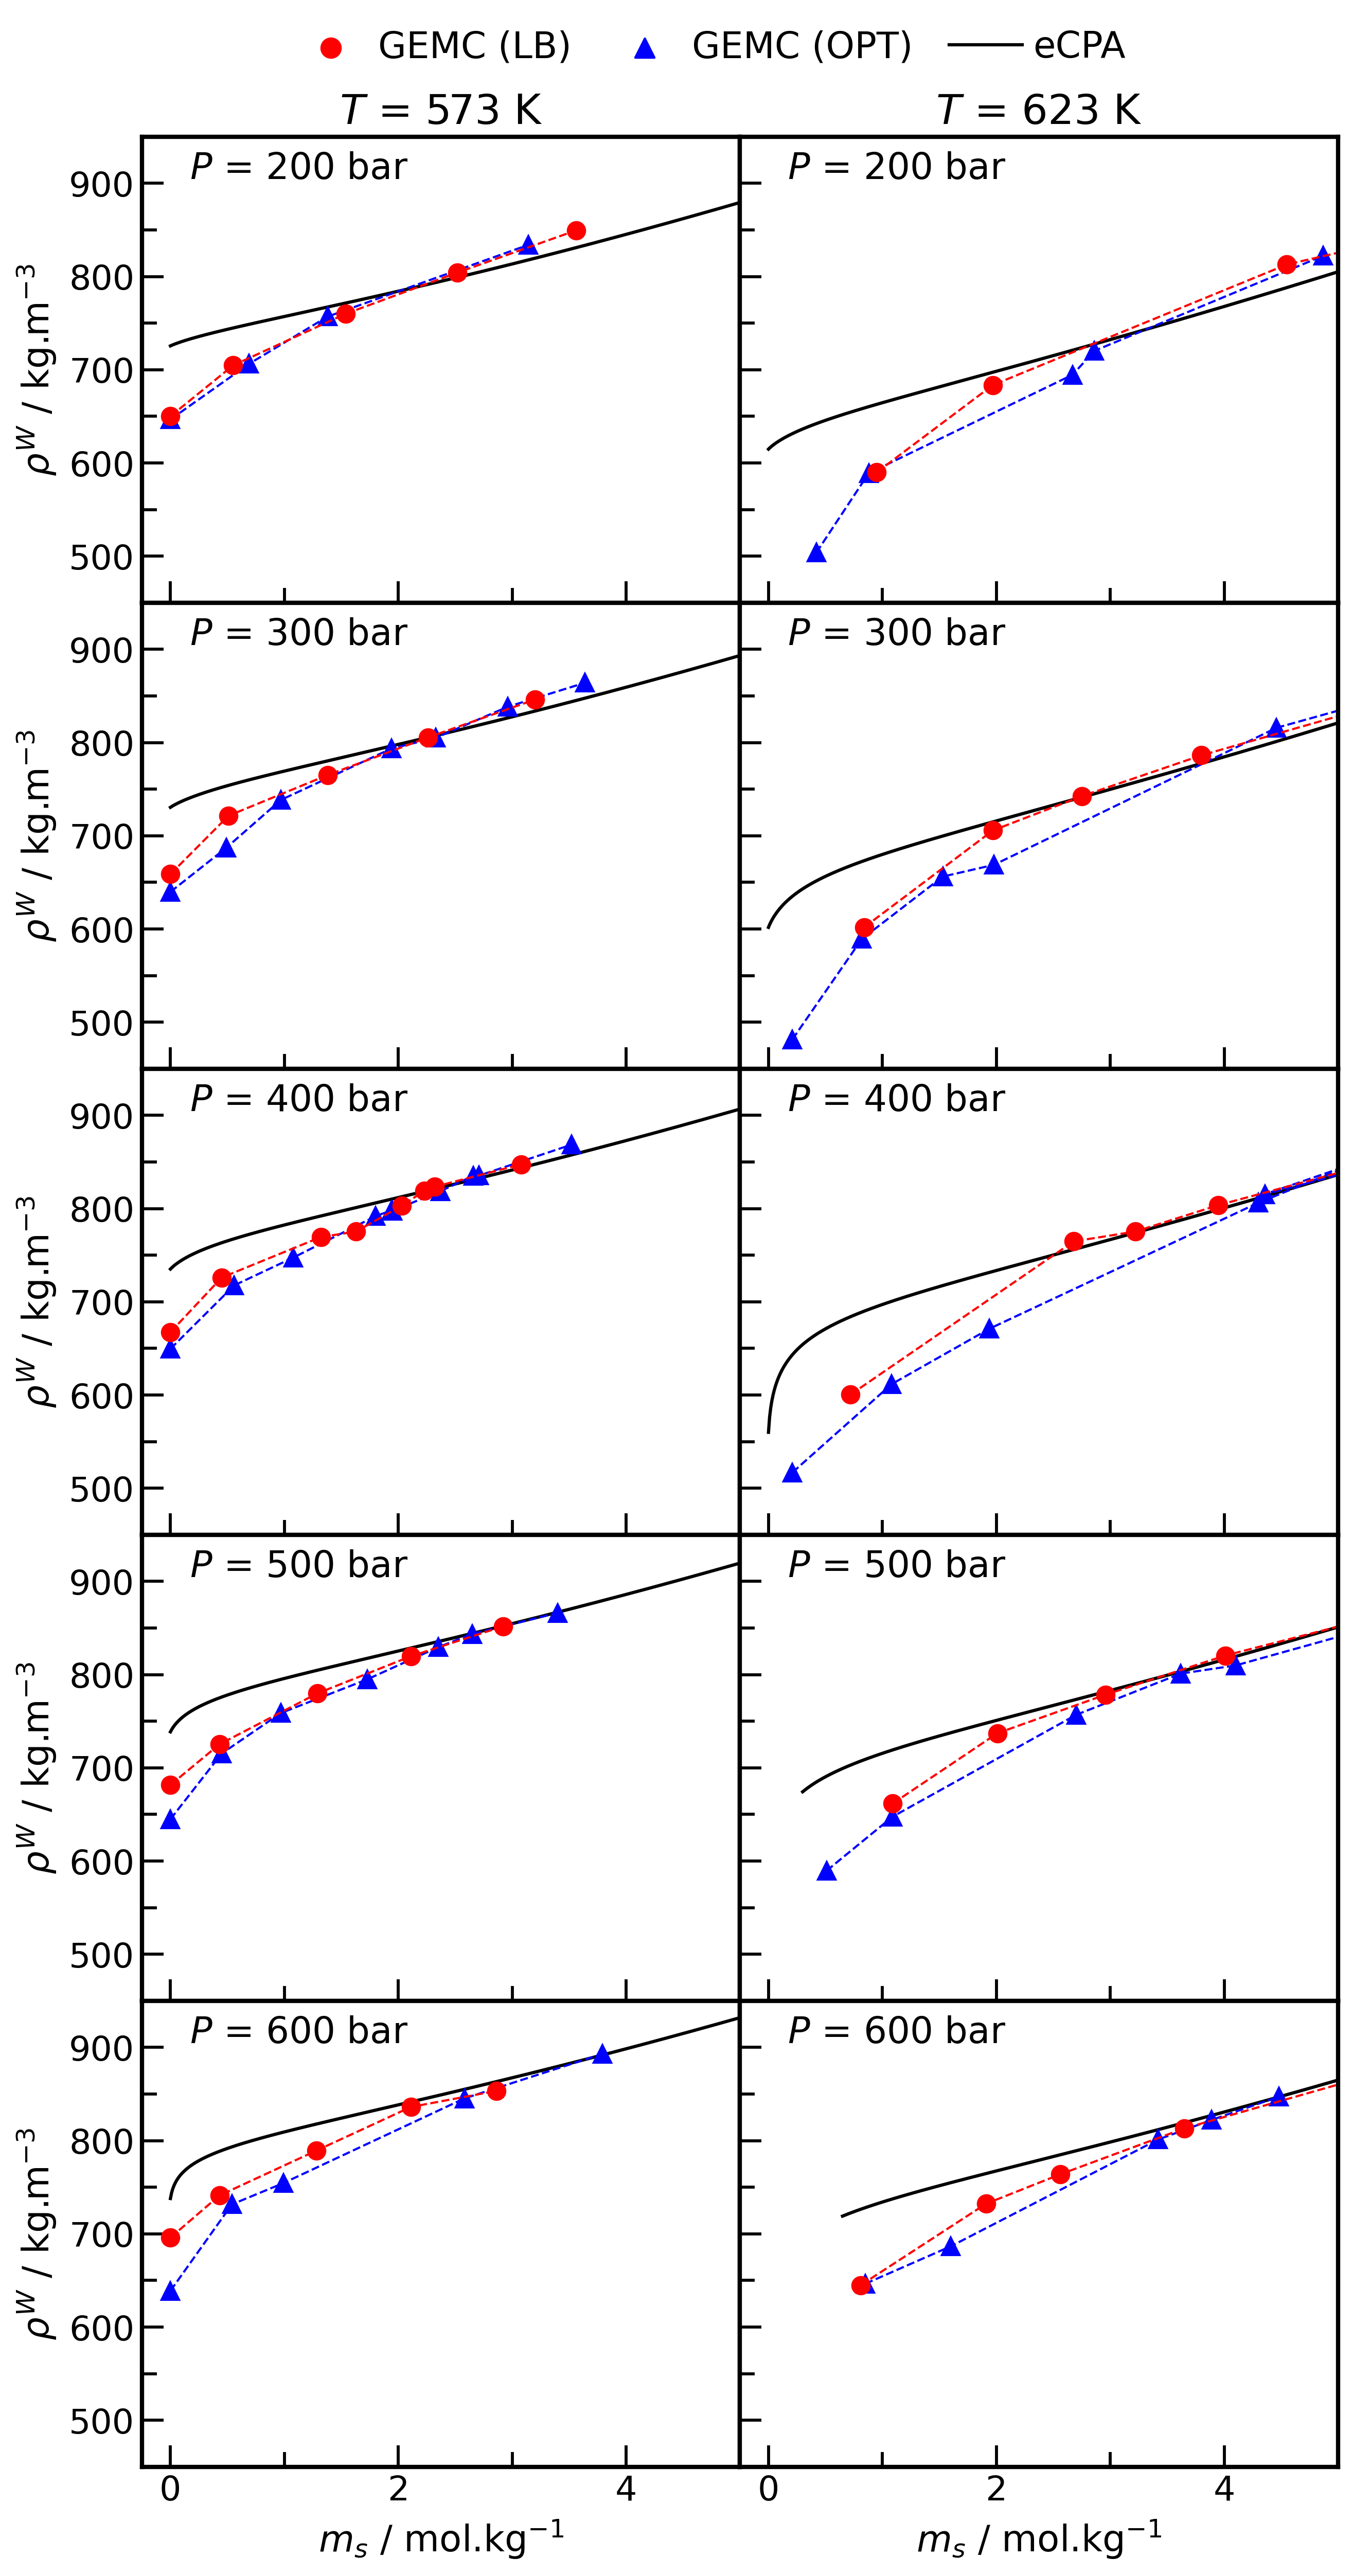
\includegraphics[width=0.55\textwidth]{Figures/rhoWGEMCvseCPA_LBvsVC.png} 
\label{GEMC_CB_rho_LBVC}
\caption{Density of the \ce{CO2}-saturated NaCl brine \textit{vs.} salt concentration at various pressures and two different temperatures from GEMC simulations and eCPA EoS. "LB" and "OPT" stand for Lorentz-Berthelot and optimized (at lower temperatures \cite{Vlcek2011}) unlike parameters between \ce{CO2}-\ce{H2O} molecules, respectively.}
\end{figure}

\newpage


\section{Association}


\begin{figure}[h!]
\centering
  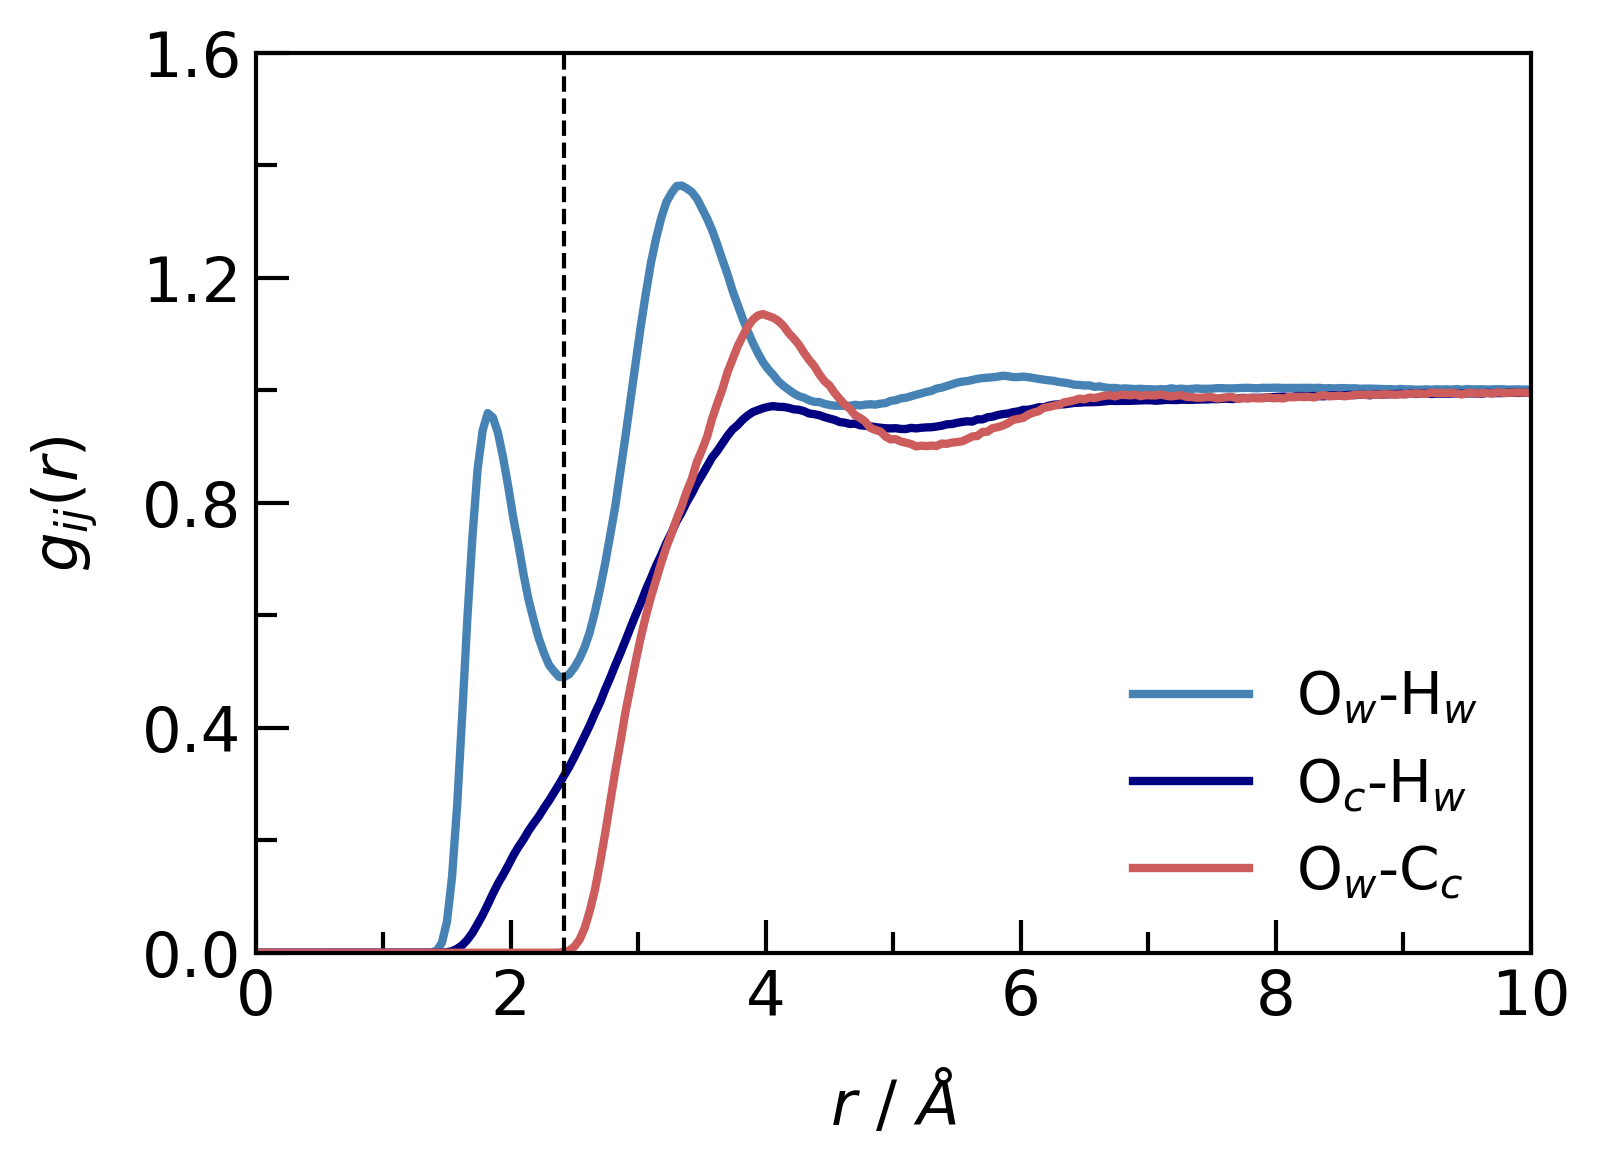
\includegraphics[width=0.45\textwidth]{Figures/gr_HBond.png} 
\caption{Scheme of the radial distribution function between the water-oxygen and water hydrogen, \ce{CO2}-oxygen and water-hydrogen, and water-oxygen and \ce{CO2}-carbon. The vertical dashed line represents the cutoff for the hydrogen bond criteria ($r = 2.4$ \AA).} 
\label{RDF}
\end{figure}


\begin{figure}[h!]
\begin{subfigure}{.49\textwidth}
  \centering
  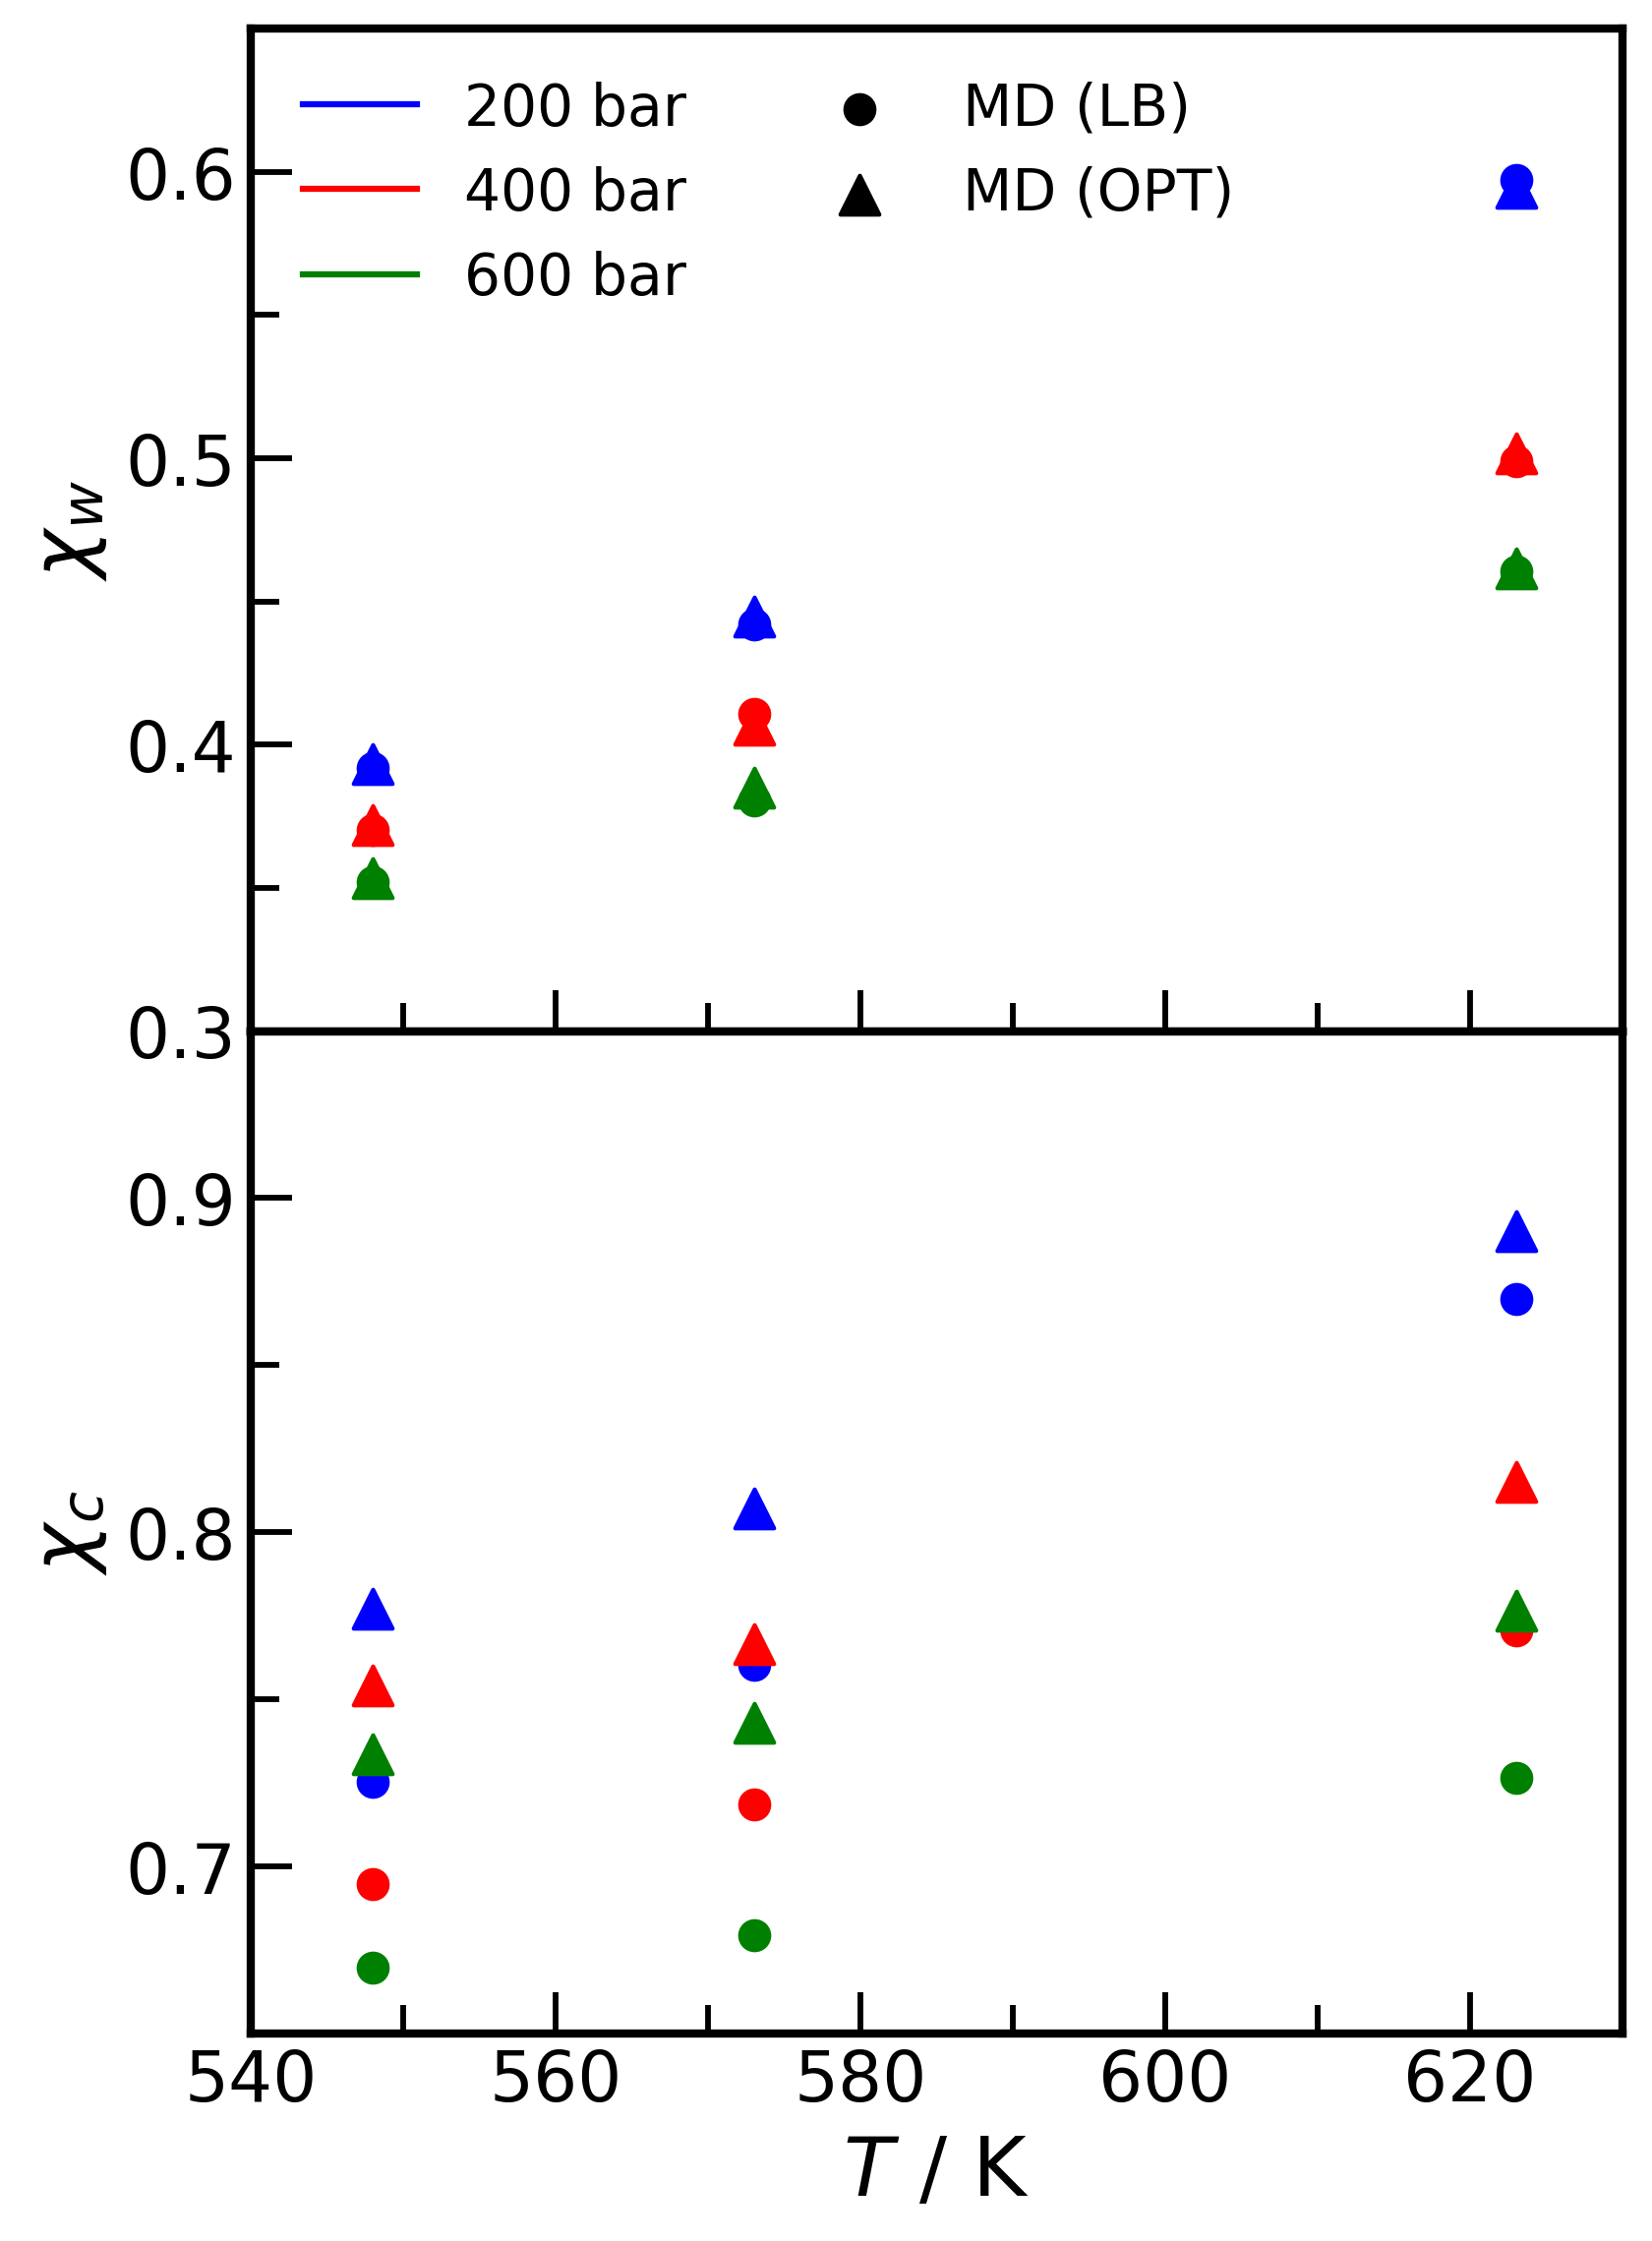
\includegraphics[width=.82\linewidth]{Figures/CW_Structure_LBvsVC_xc004.png}
  \caption{$x_c$ = 0.04}
\end{subfigure}%
\begin{subfigure}{.49\textwidth}
  \centering
  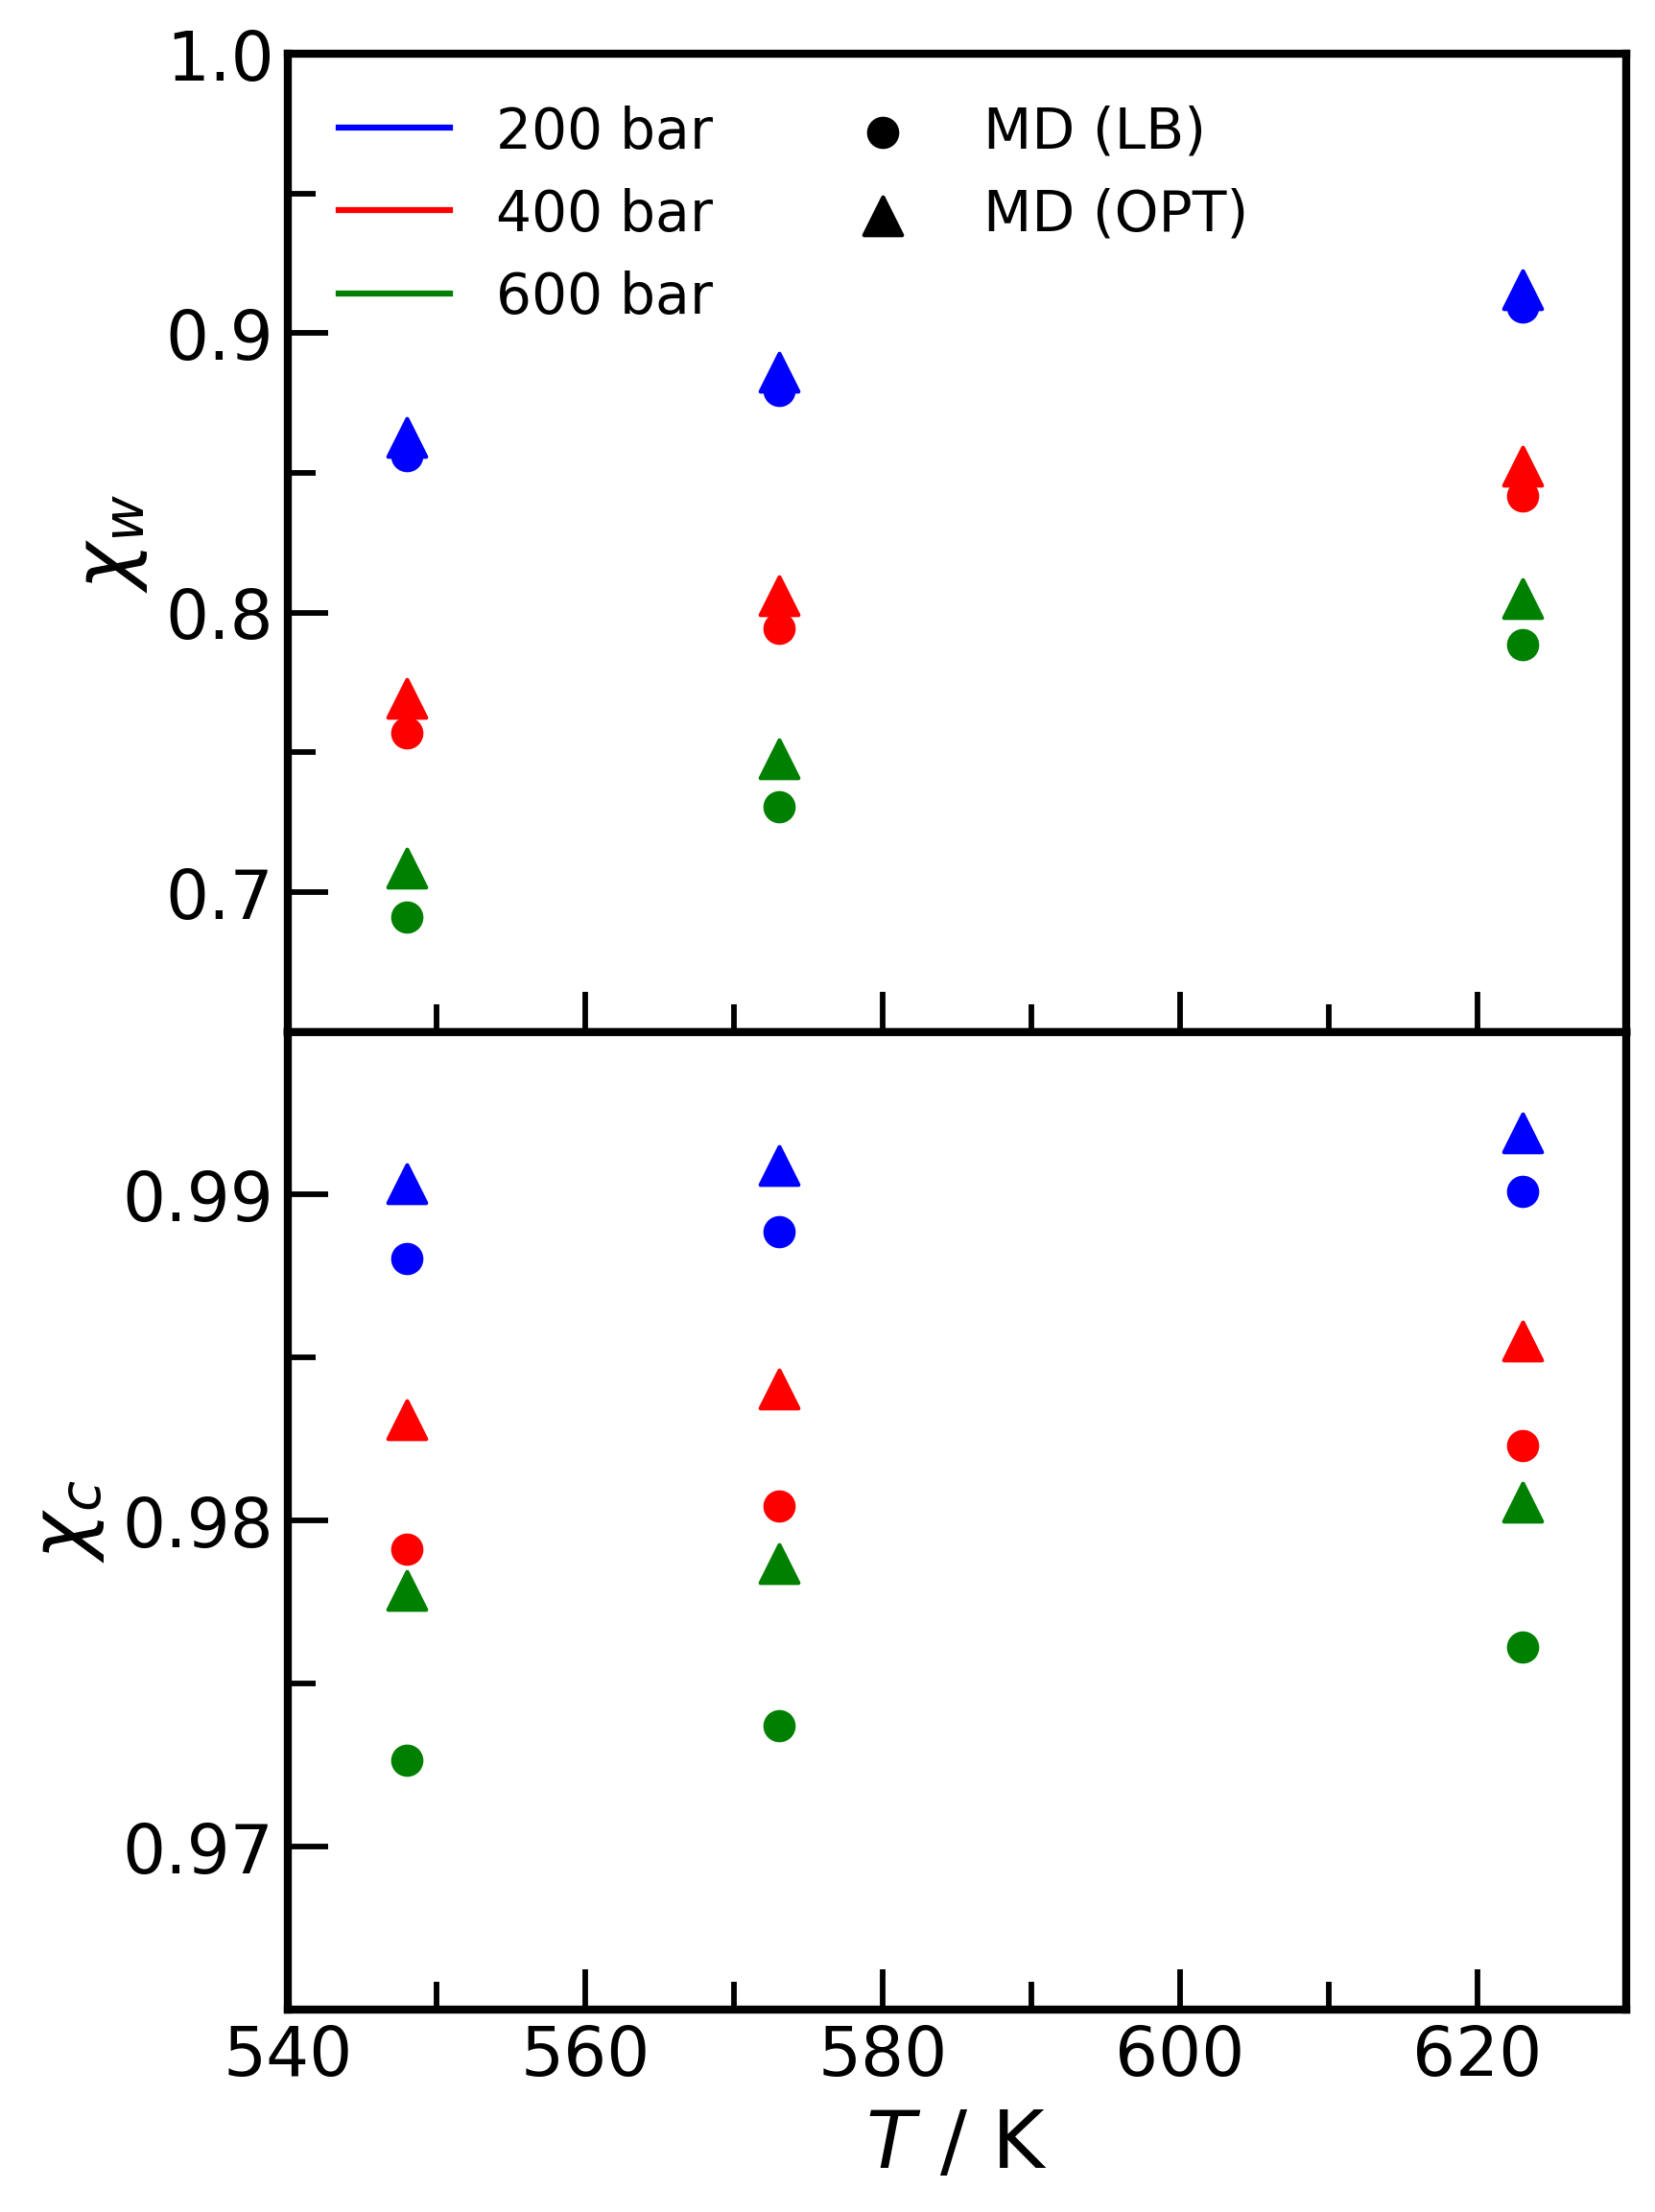
\includegraphics[width=.84\linewidth]{Figures/CW_Structure_LBvsVC_xc080.png}
  \caption{$x_c$ = 0.80}
\end{subfigure}%
\label{CHI_LB_OPT}
\caption{Association ($\chi_w$) and cross-association ($\chi_c$) in the \ce{CO2}-water mixture \textit{vs.} temperature at various pressures in (a) aqueous phase ($x_c$ = 0.04) and (b) \ce{CO2}-rich phase ($x_c$ = 0.80) from MD simulations. "LB" and "OPT" stand for Lorentz-Berthelot and optimized (at lower temperatures \cite{Vlcek2011}) unlike parameters between \ce{CO2}-\ce{H2O} molecules, respectively.} 
\end{figure}

\newpage

\begin{figure}[h!]
\begin{subfigure}{.49\textwidth}
  \centering
  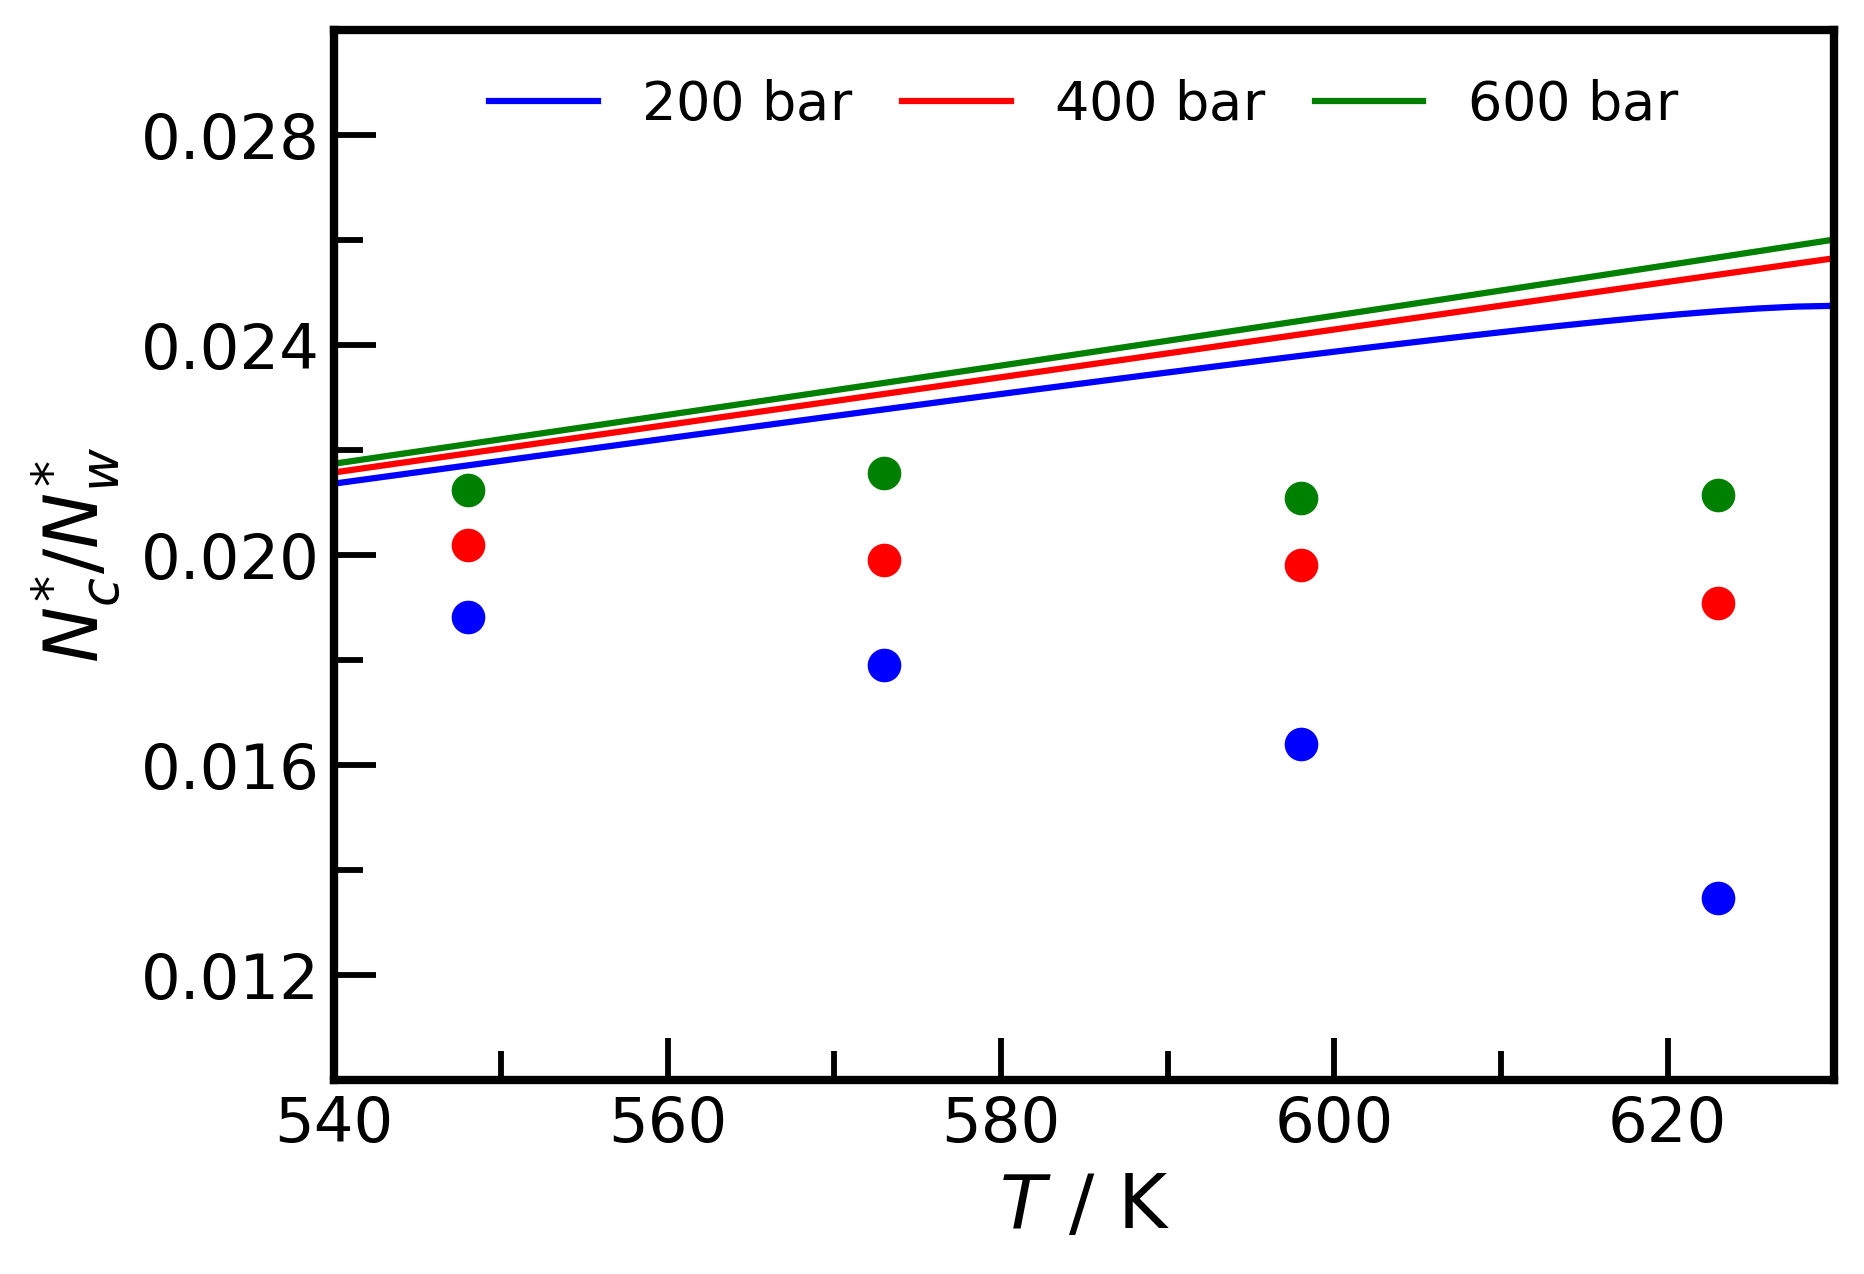
\includegraphics[width=.98\linewidth]{Figures/AssociationRatio_Aqueous.png}
  \caption{$x_c$ = 0.04}
\end{subfigure}%
\begin{subfigure}{.49\textwidth}
  \centering
  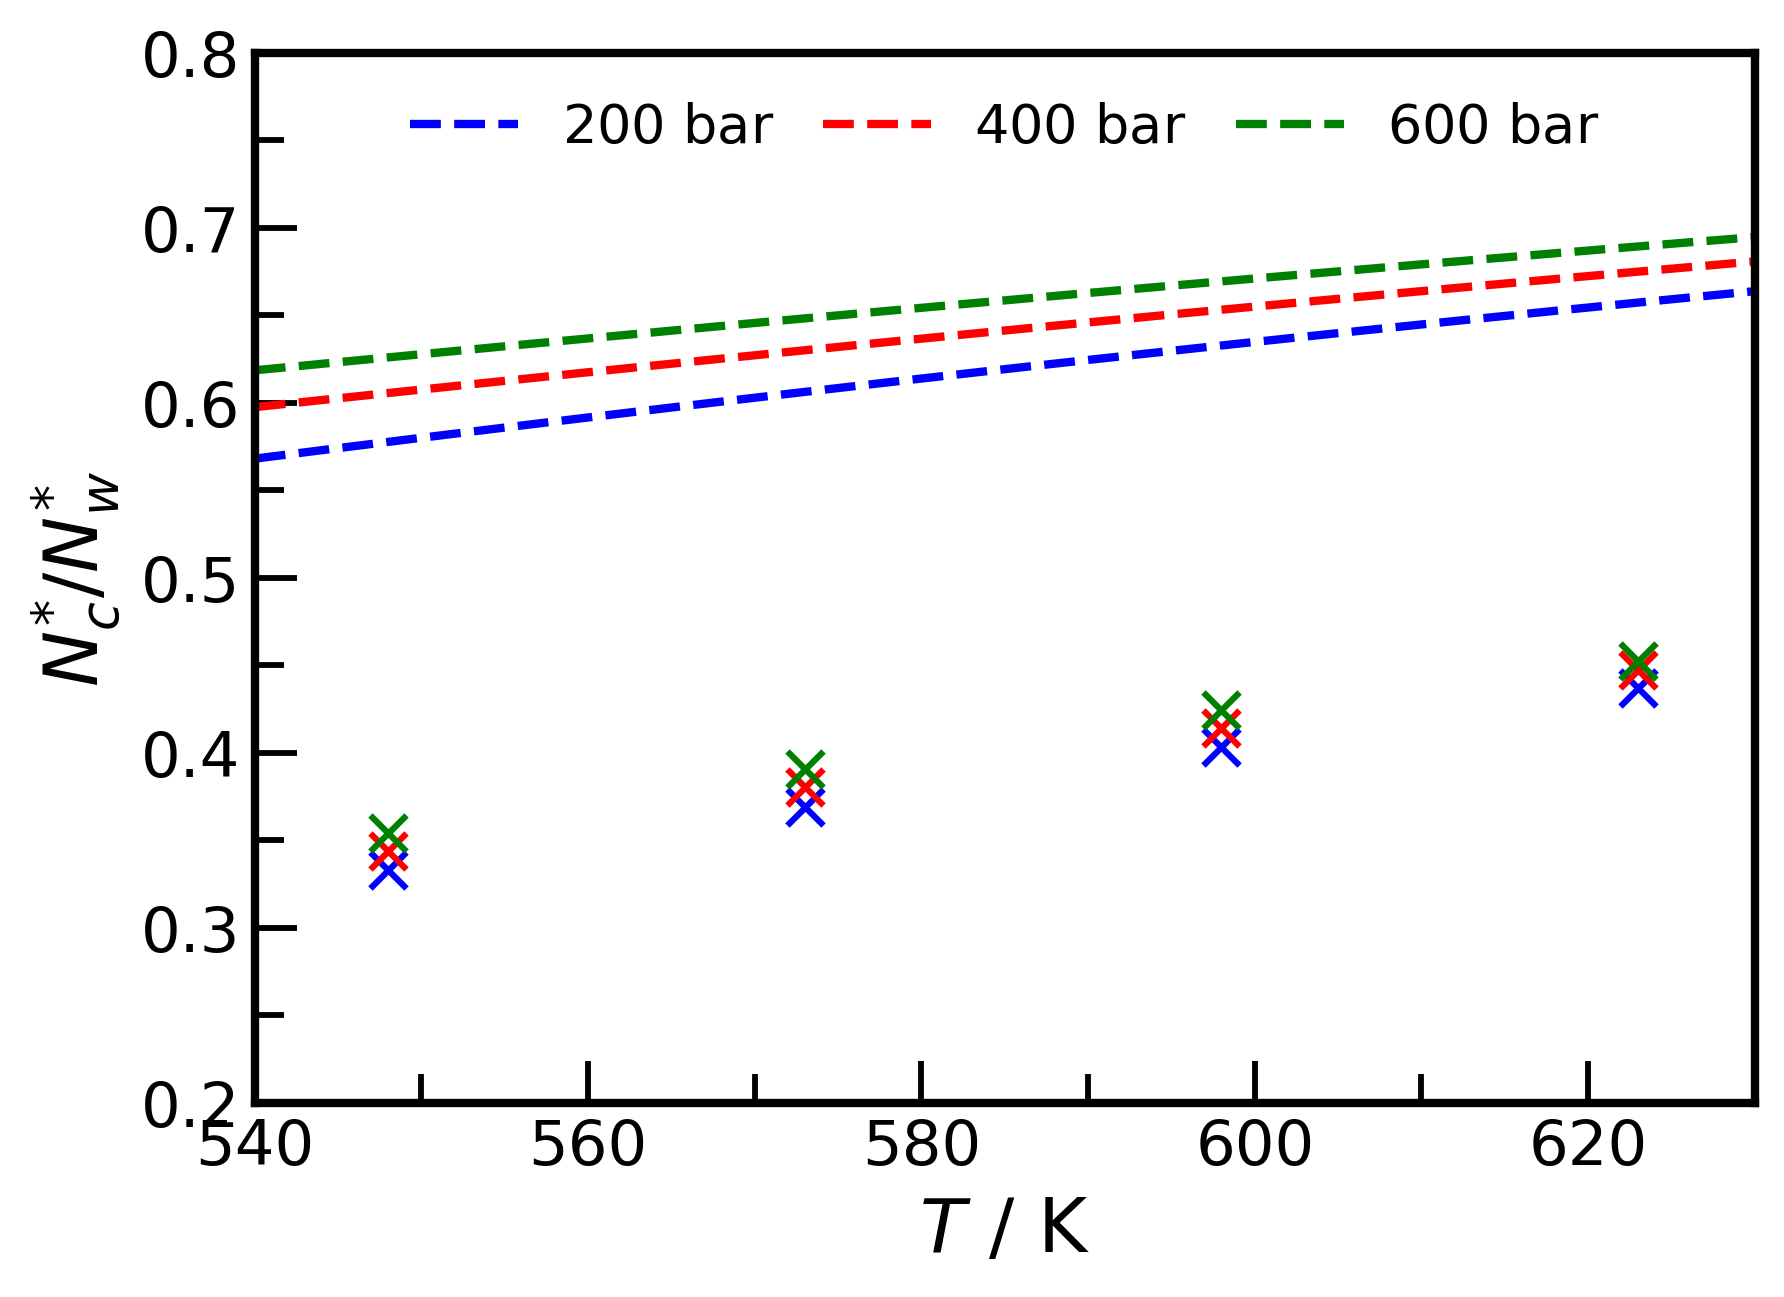
\includegraphics[width=.94\linewidth]{Figures/AssociationRatio_CO2rich.png}
  \caption{$x_c$ = 0.80}
\end{subfigure}%
\label{Assoc_Ratio}
\caption{Association ratio between the number of associating \ce{CO2} ($N_c^*$) and the number of associating \ce{H2O} ($N_w^*$) from MD simulations (discrete points) and CPA EoS (continuous line) in (a) aqueous phase ($x_c$ = 0.04) and (b) \ce{CO2}-rich phase ($x_c$ = 0.80).}
\end{figure}

\newpage